%&../.preamble

\endofdump

% \pdfcompresslevel=0
% \pdfobjcompresslevel=0
%\tcbset{shield externalize}
\usepackage{array}
\usepackage{makecell}

\usetikzlibrary{external}
\tikzset{external/system call={pdflatex --shell-escape --fmt=../.preamble --halt-on-error -jobname "\image" "\endofdump\texsource"}}
\tikzexternalize[prefix=tikz/]

% \tikzexternalize
% \tcbset{shield externalize}

\title{Algoritmi e strutture Dati}
\author{Marini Mattia}
\date{$ 1^o $ semestre $ 2^o $ anno}

\begin{document}
\maketitle
\tableofcontents
\newpage


\section{Analisi complessità}
\begin{definizione}{Criterio di costo logaritmico}
	La taglia dell’input è il \textit{numero di bit} necessari per rappresentarlo
\end{definizione}

\begin{definizione}{Criterio di costo uniforme}
	La taglia dell’input è il \textit{numero di elementi} di cui è costituito l'input
\end{definizione}

\begin{definizione}{Notazione $ O $, $ \Omega $, $ \Theta $ }
	\begin{itemize}
		\item $ O $: limita funzione \textit{dall'alto}:
		      \[
			      \exists c > 0, \exists m \in \N : \forall n \ge m,  f\left(n\right) \le c \cdot g\left(n\right)
		      \]
		\item $ \Omega $: limita funzione \textit{dal basso}:



		      \[
			      \exists c > 0, \exists m \in \N : \forall n \ge m,  f\left(n\right) \ge c \cdot g\left(n\right)
		      \]

		\item $ \Theta  $: limita funzione \textit{dal entrambe le parti}:
		      \[
			      \exists c_1, c_2 > 0, \exists m \in \N : \forall n \ge m,  c_1 \cdot g\left(n\right) \le f\left(n\right) \le c_2 \cdot g\left(n\right)
		      \]
	\end{itemize}
\end{definizione}\label{notazione ogrande}

Operativamente, per dimostrare che $ f\left(x\right) =  O\left(g\left(x\right)\right) $ oppure $ \Omega\left(g\left(x\right)\right)  $, quando $ f $ e $ g $ sono polinomi
\begin{itemize}
	\item \underline{Limite superiore $ O $}: alzo gli esponenti minori del grado di $ f $:
	      \[
		      \begin{aligned}
			      f(n) & =a_k n^k+a_{k-1} n^{k-1}+\ldots+a_1 n+a_0                                                                     \\
			           & \leq a_k n^k+\left|a_{k-1}\right| n^{k-1}+\ldots+\left|a_1\right| n+\left|a_0\right|                          \\
			           & \leq a_k n^k+\left|a_{k-1}\right| n^k+\ldots+\left|a_1\right| n^k+\left|a_0\right| n^k \quad \forall n \geq 1 \\
			           & =\left(a_k+\left|a_{k-1}\right|+\ldots+\left|a_1\right|+\left|a_0\right|\right) n^k                           \\
			           & \stackrel{?}{\leq} c n^k
		      \end{aligned}
	      \]
	      che è vera per $c \geq\left(a_k+\left|a_{k-1}\right|+\ldots+\left|a_1\right|+\left|a_0\right|\right)>0$ e per $m=1$.

	\item \underline{Limite inferiore $ \Omega  $}: alzo gli esponenti minori del grado di $ f $:

	      \[
		      \begin{aligned}
			      f(n) & =a_k n^k+a_{k-1} n^{k-1}+\ldots+a_1 n+a_0                                                                                 \\
			           & \geq a_k n^k-\left|a_{k-1}\right| n^{k-1}-\ldots-\left|a_1\right| n-\left|a_0\right|                                      \\
			           & \geq a_k n^k-\left|a_{k-1}\right| n^{k-1}-\ldots-\left|a_1\right| n^{k-1}-\left|a_0\right| n^{k-1} \quad \forall n \geq 1 \\
			           & ? \geq d n^k
		      \end{aligned}
	      \]
	      che è vera se:
	      \[
		      d \leq a_k-\frac{\left|a_{k-1}\right|}{n}-\frac{\left|a_{k-2}\right|}{n}-\ldots-\frac{\left|a_1\right|}{n}-\frac{\left|a_0\right|}{n}>0 \Leftrightarrow n>\frac{\left|a_{k-1}\right|+\ldots+\left|a_0\right|}{a_k}
	      \]
	      Nota come in questo caso alziamo gli esponenti solo a $ k-1 $ e non $ k $ in quanto, così facendo otteniamo che $ d \le h\left(x\right) $ dove $ h\left(x\right) $ p monotona decrescente. Per questo motivo esisterà per forza un $ d $ che la limita dall'alto

\end{itemize}


\begin{definizione}{Notazione $ o, \omega  $}
	\begin{itemize}
		\item $ o $: funzione limitata dall'alto:
		      \[
			      \forall c \; \exists m : f\left(n\right) < c g\left(n\right),  \forall n > m
		      \]
		\item $ \omega  $ funzione limitata dal basso:
		      \[
			      \forall c \; \exists m : f\left(n\right) > c g\left(n\right),  \forall n > m
		      \]
	\end{itemize}
	la differenza rispetto alle notazioni in definizione \ref{notazione ogrande} sta nel $ \forall c $
\end{definizione}


Utilizzando il concetto di limite, date due funzioni $f(n)$ e $g(n)$ si possono fare le seguenti affermazioni:

\[
	\begin{aligned}
		\lim _{n \rightarrow \infty} \frac{f(n)}{g(n)}=0        & \Rightarrow f(n)=o(g(n))      \\
		\lim _{n \rightarrow \infty} \frac{f(n)}{g(n)}=c \neq 0 & \Rightarrow f(n)=\Theta(g(n)) \\
		\lim _{n \rightarrow \infty} \frac{f(n)}{g(n)}=+\infty  & \Rightarrow f(n)=\omega(g(n))
	\end{aligned}
\]


Si noti che:

\begin{align*}
	f(n) & =o(g(n)) \Rightarrow f(n)=O(g(n))             \\
	f(n) & =\omega(g(n))   \Rightarrow f(n)=\Omega(g(n))
\end{align*}


\subsection{Proprietà di {$ O, \Omega , \Theta  $}}
\begin{enumerate}
	\item Dualità \label{dualità}
	\item Eliminazione delle costanti \label{eliminazione}
	\item Somma \label{somma}
	\item Prodotto \label{prodotto}
	\item Simmetria \label{simmetria}
	\item Transitività \label{transitività}
\end{enumerate}
Dimostrazioni:
\begin{enumerate}
	\item \hyperref[dualità]{Dualità}: è sufficiente girare la formula data dalla definizione  $ O\left(\right) $, ribattezzando la nuova costante $ c' = \frac{1}{c} $
	\item \hyperref[eliminazione]{Eliminazione delle costanti}: moltriplico per una nuova costante arbitraria $ a $ e ribattezzo $ c' = ac  $
	\item \hyperref[somma]{Somma}: ricordarsi che
	      \[
		      f_1\left(n\right) + f_2\left(n\right) \le \operatorname{max} \left(c_1, c_2\right) 2 \operatorname{max} \left(g_1\left(n\right), g_2\left(n\right)\right)
	      \]
	\item \hyperref[prodotto]{Prodotto}: come con somma, è immediato
	\item \hyperref[simmetria]{Simmetria}: è immediato dalla \hyperref[dualità]{dualità}
	\item \hyperref[transitività]{Transitività}: dalla catena di $ \le $ ottengo che $ f\left(n\right) \le c_1 c_2 h\left(n\right) $
\end{enumerate}


\subsection{Dimostrazione complessità}
Ci sono 3 metodi principali per l'analisi della complessità di un algoritmo:

\subsubsection{Analisi a livelli, o metodo dell'albero}\label{complessita per sostituzione}
\begin{enumerate}
	\item Srotola albero/espandi espressione e capisci la forma che ha.
	\item Di solito si ottiene una sommatoria alla fine.
	\item Risolvere sommatoria in forma chiusa secondo successioni geometriche. Le più comuni sono:
	      \begin{equation}
		      \sum_{i=0}^{k} x^{i} = \frac{x^{k+1} - 1}{x - 1}
	      \end{equation}\label{somma potenze}
\end{enumerate}


\subsubsection{ Analisi per tentativi (induzione)}
\begin{itemize}
	\item Bisogna tirare a indovinare la complessità dell'algoritmo e poi dimostrare per induzione che è vera per ogni $ n $
	\item Se il tentativo è sbagliato ci sono due opzioni:
	      \begin{itemize}
		      \item La costante $ c $ trovata dipende da $ n $, quindi non è una costante
		      \item L'equazione finale è impossibile
	      \end{itemize}
	\item Il tentativo può essere giusto però possiamo comunque fallire nella dimostrazione. In questo caso ritentare con un \textit{limite più stretto}. Ad esempio se abbiamo tentato con $ O\left(n^2 \right) $ possiamo tentare con $ O\left(n^2  - bn\right) $
	\item Può infine darsi che \textit{non si riesca a dimostrare il caso base} con $ n = 1 $. In tal caso si può dimostrare gli altri per $ n=2, \ldots , n=k $, assicurandosi che siano coperti tutti i casi per $ n<k $
\end{itemize}

\subsubsection{Metodo dell'esperto (master theorem)}
\begin{definizione}{Master theorem}
	Siano $ a $ e $ b $ costanti intere tali che $ a \geq 1 $ e $ b \geq 2 $, e $ c, \beta $ costanti reali tali che $ c > 0 $ e $ \beta \geq 0 $. Sia $ T(n) $ data dalla relazione di ricorrenza:

	\[
		T(n) =
		\begin{cases}
			aT(n/b) + cn^\beta & n > 1    \\
			d                  & n \leq 1
		\end{cases}
	\]

	Posto $ \alpha = \frac{\log a}{\log b} = \log_b a $, allora:

	\[
		T(n) =
		\begin{cases}
			\Theta(n^\alpha)        & \alpha > \beta \\
			\Theta(n^\beta  \log n) & \alpha = \beta \\
			\Theta(n^\beta)         & \alpha < \beta
		\end{cases}
	\]
\end{definizione}\label{master theorem}
Per ricordarti, pensa al fattore $ \frac{\log \left(a\right)}{\log \left(b\right)} $ come la velocità con cui "esplodono" le chiamate ricorsive. \\
Se questa è alta ($ > \beta  $) allora questa prevale e la complessità è $ \Theta \left(n^{\alpha }\right) $. \\
In caso contrario prevale il fattore $ n^{\beta } $ quindi la complessità è $ \Theta \left(n^{\beta }\right) $
\vskip3mm
La dimostrazione procede innanzitutto considerando la ricorrenza lineare generica
\[
	T(n) = aT(n/b) + cn^{\beta }
\]
Supponiamo inoltre di avere $ n $ potenza di $ b $, cioè $ n = b^k $ per qualche $ k \in \N $. In questo modo ci semplifichiamo la vita, in quanto "srotolando" la ricorrenza otteniamo un albero completo.
Cerchiamo di calcolare il costo usando il medoto dell'albero descritto in sezione \ref{complessita per sostituzione}

\begin{table}[H]
	\centering
	\begin{tabular}{ccccc}
		\toprule
		Liv.     & Dim.      & Costo chiam.      & N. chiamate & Costo livello        \\
		\midrule
		0        & $b^k$     & $cb^{k\beta}$     & 1           & $cb^{k\beta}$        \\
		1        & $b^{k-1}$ & $cb^{(k-1)\beta}$ & $a$         & $acb^{(k-1)\beta}$   \\
		2        & $b^{k-2}$ & $cb^{(k-2)\beta}$ & $a^2$       & $a^2cb^{(k-2)\beta}$ \\
		$\ldots$ & $\ldots$  & $\ldots$          & $\ldots$    & $\ldots$             \\
		$i$      & $b^{k-i}$ & $cb^{(k-i)\beta}$ & $a^i$       & $a^icb^{(k-i)\beta}$ \\
		$\ldots$ & $\ldots$  & $\ldots$          & $\ldots$    & $\ldots$             \\
		$k-1$    & $b$       & $cb^{\beta}$      & $a^{k-1}$   & $a^{k-1}cb^{\beta}$  \\
		$k$      & 1         & $d$               & $a^k$       & $da^k$               \\
		\bottomrule
	\end{tabular}
\end{table}
Dunque, possiamo arrivare alla conclusione che la somma di tutti i livelli, ossia la \textit{complessitò complessiva} dell'algoritmo, è data da:
\[
	T\left(n\right) = a^{k} d + c b ^{k \beta }  \sum_{i=0}^{k-1} \left(\frac{a}{b^{\beta }}\right)^{i}
\]

Prima di partire dobbiamo fare due \sfblue{importanti osservazioni}:
\begin{align*}
	a^{k} = n^{\alpha} &  & a = b^{\alpha}
\end{align*}

\begin{tcolorbox}
	\sfblue{Caso 1}: $ \alpha > \beta $
	\tcblower
	\vskip3mm
	Ne segue che $q = b^{\alpha-\beta} > 1:$

	\begin{align*}
		T(n) & = dn^{\alpha} + cb^{k\beta} \sum_{i=0}^{k-1} q^i                                    &                                           \\
		     & = n^{\alpha}d + cb^{k\beta}\textcolor{mutedred}{\left[\frac{q^k - 1}{q - 1}\right]} & \text{Serie geometrica finita}            \\
		     & \leq n^{\alpha}d + cb^{k\beta}\textcolor{mutedred}{\frac{q^k}{q - 1}}               & \text{Disequazione}                       \\
		     & = n^{\alpha}d + \frac{cb^{k\beta}a^k}{b^{k\beta}}/(q - 1)                           & \text{Sostituzione } q                    \\
		     & = n^{\alpha}d + ca^k/(q - 1)                                                        & \text{Passi algebrici}                    \\
		     & = n^{\alpha}[d + c/(q - 1)]                                                         & a^k = n^{\alpha}, \text{raccolta termini}
	\end{align*}
	Dunque
	\[
		T(n) = \Theta (n^{\alpha})
	\]
\end{tcolorbox}
\vskip3mm
Ho usato il fatto che $ q > 1 $ nel passaggio evidenziato in rosso. Pensa così:
\[
	\frac{q^{k}-1}{q-1} \quad  \text{ sempre } > 0
\]
mentre
\[
	\frac{q^{k}}{q-1}
	\begin{cases}
		> 0 \text{ se }  q > 1 \\
		< 0 \text{ se }  q < 1 \\
	\end{cases}
\]


\vskip3mm

\begin{tcolorbox}
	\sfblue{Caso 2}: $ \alpha = \beta $
	\tcblower
	Ne segue che:  $q = b^{\alpha-\beta} = 1$

	\begin{align*}
		T(n) & = dn^{\alpha} + cb^{k\beta} \sum_{i=0}^{k-1} q^i                                   \\
		     & = n^{\alpha}d + cn^{\beta} \textcolor{mutedred}{k}       & q^i = 1^i = 1           \\
		     & = n^{\alpha}d + cn^{\alpha}k                             & \alpha = \beta          \\
		     & = n^{\alpha}(d + ck)                                     & \text{Raccolta termini} \\
		     & = n^{\alpha}[d + c\textcolor{mutedred}{\log n / \log b}] & k = \log_b n
	\end{align*}

	Dunque
	\[
		T(n) = \Theta(n^{\alpha} \log n)
	\]

	\vskip3mm

\end{tcolorbox}

\begin{tcolorbox}
	\sfblue{Caso 3}: $ \alpha < \beta $
	Ne segue che:  $q = b^{\alpha-\beta} < 1$
	\tcblower
	\begin{align*}
		T(n) & = dn^{\alpha} + cb^{k\beta} \sum_{i=0}^{k-1} q^i                                                      \\
		     & = n^{\alpha}d + cb^{k\beta}\textcolor{mutedred}{[(q^k - 1)/(q - 1)]} & \text{Serie geometrica finita} \\
		     & = n^{\alpha}d + cb^{k\beta}\textcolor{mutedred}{[(1 - q^k)/(1 - q)]} & \text{Inversione}              \\
		     & \leq n^{\alpha}d + cb^{k\beta}\textcolor{mutedred}{[1/(1 - q)]}      & \text{Disequazione}            \\
		     & = n^{\alpha}d + cn^{\beta}/(1 - q)                                   & b^k = n
	\end{align*}

	Dunque
	\[
		T(n) = \Theta (n^{\beta})
	\]
\end{tcolorbox}

\subsubsection{Versione generalizzata}
\begin{definizione}{Master theorem generalizzato}
	Sia $ a \geq 1 $, $ b > 1 $, $ f(n) $ asintoticamente positiva, e sia

	\[
		T(n) =
		\begin{cases}
			aT(n/b) + f(n) & n > 1    \\
			d              & n \leq 1
		\end{cases}
	\]

	Sia $ \alpha = \frac{\log \left(a\right)}{\log \left(b\right)} \log_b a $. Sono dati tre casi:



	\newsavebox{\tmp}
	\savebox{\tmp}{%
		$
			\begin{aligned}
				 & \exists \epsilon > 0 : f(n) = \Omega(n^{\alpha + \epsilon}) \wedge \\
				 & \exists c : 0 < c < 1, \exists m \geq 0 :                          \\
				 & af(n/b) \leq c f(n), \forall n \geq m                              \\
			\end{aligned}
		$
	}

	\begin{center}
		\begin{tabular}{ll}
			\toprule
			Caso                                                     & complessità                   \\
			\midrule
			$\exists \epsilon > 0 : f(n) = O(n^{\alpha - \epsilon})$ & $ T(n) = \Theta(n^\alpha)$    \\
			$f(n) = \Theta(n^\alpha)$                                & $ T(n) = \Theta(f(n) \log n)$ \\
			\usebox{\tmp}                                            & $ T(n) = \Theta(f(n))$        \\
			\bottomrule
		\end{tabular}
	\end{center}

\end{definizione}
\subsection{Ricorrenze lineari}
\begin{definizione}{Ricorrenze lineari}
	Siano $a_1, a_2, \dots, a_h$ costanti intere non negative, con $h$ costante positiva, $c$ e $\beta$ costanti reali tali che $c > 0$ e $\beta \geq 0$, e sia $T(n)$ definita dalla relazione di ricorrenza:

	\[
		T(n) =
		\begin{cases}
			\sum_{1 \leq i \leq h} a_i T(n - i) + c n^\beta & n > m           \\
			\Theta(1)                                       & n \leq m \geq h
		\end{cases}
	\]

	Posto $a = \sum_{1 \leq i \leq h} a_i$, allora:

	\begin{itemize}
		\item \quad $T(n)$ è $\Theta(n^{\beta+1})$, se $a = 1$.
		\item \quad $T(n)$ è $\Theta(a^n n^\beta)$, se $a \geq 2$.
	\end{itemize}
	\vskip3mm
\end{definizione}

\section{Analisi ammortizzata}
L'analisi ammortizzata è utile nel caso in cui la complessità di un algoritmo dipende dallo "stato" di una struttura dati associata. Ci sono 3 metodi:
\begin{itemize}
	\item \sfblue{Metodo dell'aggregazione}: si calcola il costo totale di $ n $ operazioni e si divide per $ n $.
	\item \sfblue{Metodo degli accantonamenti}: alle operazioni vengono assegnati i \textit{costi ammortizzati}, che possono essere maggiori/minori del loro costo effettivo
	\item \sfblue{Metodo del potenziale} Lo stato del sistema viene rappresentato da una \textit{funzione di potenziale}
\end{itemize}

\subsubsection{Contatore binario (metodo dell'aggregazione)}
Immaginiamo di avere un contatore binario con l'algoritmo  {\ttfamily increment} che . Questo algoritmo avrà complessità che dipende molto dal numero di 1 che deve scorrere


\vskip3mm
\begin{algoritmo*}{Increment}
	\begin{algorithm}[H]
		% \caption{increment binary counter}
		\SetKwFunction{Increment}{\Void increment}
		\Fn{ \Increment{$\Bool[]\ A$, $\Int\ k$}}{
			$i \gets 0$\;
			\While{$i < k$ \And $A[i] = 1$}{
				$A[i] \gets 0$\;
				$i \gets i + 1$\;
			}
			\If{$i < k$}{
				$A[i] \gets 1$\;
			}
		}
	\end{algorithm}
\end{algoritmo*}
\vskip3mm

Nota come il bit $ i $ -esimo viene modificato ogni $ 2^{i} $ incrementi. Per questo il costo di $ n $ operazioni consecutive è di:
\[
	\text{ Costo totale }: \sum_{i=0}^{k-1} \left\lfloor \frac{n}{2^{i}} \right\rfloor \le n \sum_{i=0}^{k-1} \frac{1}{2^{i}} \le n \sum_{i=0}^{\infty} \frac{1}{2^{i}} = 2n
\]
Dunque il costo ammortizzato secondo il metodo dell'aggregazione è di:
\[
	\text{ Costo ammortizzato }: \frac{T\left(n\right)}{n} \le \frac{2n}{n} = O\left(1\right)
\]
\subsubsection{Contatore binario (metodo degli accantonamenti)} \label{metodo accantonamenti}
Possiamo stimare il costo necessario per una singola iterazione dell'algoritmo. Sapredo dunque che il costo ammortizzato può essere maggiore o minore del costo effettivo. Su $ n $ iterazioni tuttavia, sappiamo che il coto effettivo di queste sarà sempre minore
\vskip3mm
Nel caso del contatore binario possiamo assegnare un costo ammortizzato di $ 2 $ per ogni operazione. In questo modo, ogni bit impostato a 1 ha "immagazzinato" un'operazione bonus che può essere usata per riportare il bit a 0, nel momento in cui devo "scorrere i bit" a sinistra. Quindi ho che:
\[
	\sum_{i=0}^{n} c_i \le \sum_{i=0}^{n} a_i = 2n
\]

\subsubsection{Contatore binario (metodo del potenziale)}
In questo caso definiamo una funzione $ \Phi\left(S\right) $ che in modo simile al metodo degli accantonamenti \ref{metodo accantonamenti} tiene traccia di quanto lavoro possiamo fare prima di eccedere la complessità stimata.
\[
	a_i = c_i + \Phi \left(S_i\right) - \Phi \left(S_{i-1}\right)
\]
siccome
\[
	A = \sum_{i = 1}^{n} a_i = C + \Phi \left(S_n\right) - \Phi \left(S_0\right)
\]
so che se $ \Phi \left(S_n\right) - \Phi \left(S_0\right) \ge 0 \rightarrow $ il costo ammortizzato è un limite superiore del costo reale
\vskip3mm
Nel caso del contatore binario:
\begin{itemize}
	\item $ \Phi \left(S\right) $ è il numero di bit settati a 1
	\item Chiamando $ t $ il numero di bit impostati a 1 prima del primo 0, abbiamo che
	      \[
		      a_i = \underbracket[0.1ex]{t+1}_{c_i} + \underbracket[0.1ex]{1-t}_{\Delta \Phi } = 2
	      \]
	\item Siccome $ \Phi \left(S_n\right) - \Phi \left(S_0\right) \ge 0  $ (ci sono più 1 nello stato finale che in quello iniziale), allora vale che
	      \[
		      T\left(n\right) = O\left(2n\right) = O\left(n\right)
	      \]
\end{itemize}
\subsection{Vettori dinamici}
L'analisi ammortizzata è fondamentale per la comprensione dei vettori dinamici.
\subsubsection{Ingrandimento}
Ho due strategie per implemetarli:
\begin{itemize}
	\item \sfblue{Strategia del raddoppiamento}: quando il vettore è pieno, raddoppio la sua dimensione (o moltiplichi per fattore specificato). Risolvendo con formula \ref{somma potenze}
	      \[
		      \text{ Costo } n \text{ inserimenti } = T\left(n\right) = n + \sum_{j=0}^{\left\lfloor \log n \right\rfloor }  2^{j} = O\left(n\right)
	      \]
	      la complessità ammortizzata è quindi:
	      \[
		      \frac{O\left(n\right)}{n} = O\left(1\right)
	      \]
	\item \sfblue{Strategia dell'ingrandimento}: quando il vettore è pieno, aggiungo un numero fisso di elementi. Dato $ d $ il fattore di ingrandimento e risolvendo la sommatoria con \textit{formula di Gauss}
	      \[
		      \text{ Costo } n \text{ inserimenti } = T\left(n\right) = n + \sum_{j=0}^{\left\lfloor n/d \right\rfloor }  d \cdot j = O\left(n^2 \right)
	      \]
	      la complessità ammortizzata è quindi:
	      \[
		      \frac{O\left(n^2 \right)}{n} = O\left(1\right)
	      \]
\end{itemize}

\subsubsection{Cancellazione}
Definiamo con
\[
	\alpha = \frac{\text{ dimensione }}{\text{ capacità }}
\]
il fattore di carico.
\begin{itemize}
	\item Impostiamolo a $ \frac{1}{4} $
	\item   (1/2  non va bene in quanto se continuiamo a inserire/rimuovere a size/2 dobbiamo continuare a riallocare il vettore)
\end{itemize}
Impostiamo una funzione di potenziale tale per cui:
\begin{itemize}
	\item Vale 0 quando $ \alpha = \frac{1}{2} $
	\item Vale \verb|dim| quando $ \alpha  = \frac{1}{4} $ o $ \alpha  = 1 $. Questo significa che posso ripagare allocazione
\end{itemize}
\[
	\Phi =
	\begin{cases}
		2 \cdot \text{ dim } - \text{ capacità } & \alpha \geq \frac{1}{2} \\
		\frac{\text{capacità}}{2} - \text{ dim } & \alpha \leq \frac{1}{2}
	\end{cases}
\]

\begin{itemize}
	\item $\alpha = \frac{1}{2}$ (dopo espansione/contrazione) $\Rightarrow$ \(\Phi = 0\)
	\item $\alpha = 1$ (prima di espansione) $\Rightarrow \text{ dim } = \text{ capacità } \Rightarrow \Phi = \text{ dim } $
	\item $\alpha = \frac{1}{4}$ (prima di contrazione) $\Rightarrow \text{ capacità } = 4 \cdot \text{ dim } \Rightarrow \Phi = \text{ dim }$
\end{itemize}

\section{Alberi}
\subsection{Alberi di ricerca binaria}
Ho le seguenti operazioni:
\subsubsection{Stampa}
Itero ricorsivamente su ogni nodo, partendo dalla radice, e stampo il valore del nodo.
Ho 3 opzioni:
\begin{itemize}
	\item \sfblue{Inorder}: stampo il sottoalbero sinistro, il nodo corrente, e il sottoalbero destro. In questo modo ottengo i nodi in ordine crescente (\sfblue{l - p - r})
	\item \sfblue{Preorder}: stampo il nodo corrente, il sottoalbero sinistro, e il sottoalbero destro. In questo modo ottengo i nodi in ordine di visita (\sfblue{p - l - r})
	\item \sfblue{Postorder}: stampo il sottoalbero sinistro, il sottoalbero destro, e il nodo corrente. In questo modo ottengo i nodi in ordine di visita, ma dopo aver visitato i figli (\sfblue{l - r - p})
\end{itemize}
\subsubsection{Ricerca}\label{bt ricerca}
\begin{itemize}
	\item Se \verb|curr.val == n.val| ho trovato il nodo
	\item Se \verb|curr.val == nil| NON ho trovato il nodo
	\item Se \verb|n.val < curr.val| chiamo ricorsivamente a sinistra
	\item Se \verb|n.val > curr.val| chiamo ricorsivamente a destra
\end{itemize}

\subsubsection{Inserimento}
Prendo un nodo \verb|new_node| e:
\begin{itemize}
	\item Se \verb|new_node.val < v.val|  chiamo ricorsivamente a sinistra
	\item Se \verb|new_node.val > v.val|  chiamo ricorsivamente a destra
	\item Altrimenti, se \verb|v.val == nil|, sono in una foglia e inserisco nodo
\end{itemize}

\subsubsection{Successore-predecessore}
Voglio trovare il nodo che viene subito prima/dopo al nodo \verb|n| nell'ordinamento. Innanzitutto trovo il nodo \verb|n| con la tecnica specificata in \ref{bt ricerca}. Supponiamo di cercare il \textit{successore}. Distinguo i due casi
\begin{itemize}
	\item Il figlio destro di \verb|n| è diverso da \verb|nil|: il successore è il nodo con il valore minimo del sottoalbero destro di \verb|n|
	\item Il figlio destro di \verb|n| è \verb|nil|:
	      \begin{itemize}
		      \item Risalgo per i parents finche non trovo un nodo che è un \textit{figlio sinistro}
		      \item Il parent di questo nodo è il \textit{successore}
	      \end{itemize}
\end{itemize}
Il ragionamento è del tutto analogo per il predecessore, ma devo considerare gli alberi a sinistra. Dunque è del tutto speculare
\vskip3mm
\begin{minipage}[t]{0.48\textwidth}
	\begin{center}
		\begin{forest}
			for tree={draw,circle, inner sep=5pt, grow = -90}
			[ u,thick
			[
			[y,phantom]
				[
					[y,phantom]
						[, edge={dashed}
								[y,phantom]
								[v, thick]
						]
				]
			]
			[y,phantom]
			]
		\end{forest}
		\vskip3mm
		$ u $ = successor ($ v $)
	\end{center}
\end{minipage}
%
\begin{minipage}[t]{0.48\textwidth}
	\begin{center}
		\begin{forest}
			for tree={draw,circle, inner sep=5pt, grow = -90}
			[ u,thick
			[y,phantom]
			[
			[
					[, edge={dashed}
								[v, thick]
								[y,phantom]
						]
						[y,phantom]
				]
				[y,phantom]
			]
			]
		\end{forest}
		\vskip3mm
		$ u $ = predecessor ($ v $)
	\end{center}
\end{minipage}

\subsubsection{Rimozione}\label{bst rimozione}
Trovo nodo da rimuovere e distinguo in 2 casi:
\begin{itemize}
	\item Se il nodo ha 0 figli, lo rimuovo semplicemente
	\item Se il nodo ha solo un figlio, posso attaccarlo al parent del nodo rimosso (\textit{shortcut})
	\item Se il nodo ha 2 figli, allora:
	      \begin{itemize}
		      \item Noto che il successore è per forza nel sottoalbero destro. Se il sottoalbero destro esiste allora non serve ricercare il successore nei parents
		      \item Trovo il successore \verb|s|. Nota che il successore non può avere un figlio sinistro perché deve essere il minimo del sottoalbero destro
		      \item Se il successore ha un figlio destro, lo attacco al parent del successore (\textit{shortcut})
		      \item Sostituisco il valore del nodo da rimuovere con il valore del successore
	      \end{itemize}
\end{itemize}



\subsection{Alberi red-black}
Gli alberi red black sono alberi binari il cui scopo è \textit{mantenere il bilanciamento dell'albero} dopo ogni inserimento. In realtà, non è garantito che l'albero sia sempre completamente bilanciato, ma la differenza di altezza può essere al più $ \log \left(n\right) $. In un albero red-black ogni nodo è di colore rosso o nero.

\vskip3mm
In un RBT vigono le seguenti proprietà:
\begin{itemize}
	\item La radice è nera
	\item Ogni foglia è nera ed è un "nodo nil"
	\item Se un nodo è rosso, allora entrambi i suoi figli sono neri
	\item Ogni cammino da un nodo a una foglia ha lo stesso numero di nodi neri (altezza nera)
\end{itemize}
\subsubsection{Inserimento}
Per capire l'inserimento, bisogna definire le operazioni di \underline{rotazione}:
\vskip3mm
\begin{minipage}[t]{0.48\textwidth}
	\begin{center}
		\begin{forest}
			for tree={draw,circle, grow = -90}
			[
			p
				[x
						[A, isosceles triangle, shape border rotate=90, child anchor=parent]
						[y
								[B, isosceles triangle, shape border rotate=90, child anchor=parent]
								[C, isosceles triangle, shape border rotate=90, child anchor=parent]
						]
				]
				[y,phantom]
			]
		\end{forest}
	\end{center}
\end{minipage}
%
\begin{minipage}[t]{0.48\textwidth}
	\begin{center}
		\begin{forest}
			for tree={draw,circle, grow = -90}
			[p
				[y
						[x
								[A, isosceles triangle, shape border rotate=90, child anchor=parent]
								[B, isosceles triangle, shape border rotate=90, child anchor=parent]
						]
						[C, isosceles triangle, shape border rotate=90, child anchor=parent]
				]
				[y,phantom]
			]
		\end{forest}
	\end{center}
\end{minipage}
\vskip3mm
Nota come dopo la rotazione, il sorting dei nodi non cambia ([A, x, B, y, C, p])
\vskip3mm
Nell'inserimento, si imposterà il colore del nuovo nodo a rosso (non posso violare vincolo altezza nera), e fixo ricorsivamente le violazioni di vincoli che si possono creare. In particolare ci sono 7 casi:

\begin{itemize}
	\item \sfblue{Caso1}: nodo non ha padre: zero problemi, cambio colore in nero
	\item \sfblue{Caso2}: nodo ha padre nero: zero problemi, nessun vincolo è violato
	\item \sfblue{Caso3}: $ t $ rosso, $ p $ rosso, $ z $ rosso. Semplicemente cambio colore di $ p $ e $ z $
	      \vskip3mm
	      \begin{minipage}[t]{0.48\linewidth}
		      \begin{center}
			      \begin{forest}
				      for tree={draw,circle, grow = -90}
				      [
				      n, fill=black!50, text=white
				      [p, fill=mutedred!50, text=white
				      [t, fill=mutedred!50, text=white
				      [A, isosceles triangle, draw, shape border rotate=90, child anchor=parent]
				      [B, isosceles triangle, draw, shape border rotate=90, child anchor=parent]
				      ]
				      [C, isosceles triangle, draw, shape border rotate=90, child anchor=parent]
				      ]
				      [z, fill=mutedred!50, text=white
				      [D, isosceles triangle, draw, shape border rotate=90, child anchor=parent]
				      [E, isosceles triangle, draw, shape border rotate=90, child anchor=parent]
				      ]
				      ]
			      \end{forest}
		      \end{center}
	      \end{minipage}
	      %
	      \begin{minipage}[t]{0.48\linewidth}
		      \begin{center}
			      \begin{forest}
				      for tree={draw,circle, grow = -90}
				      [n, fill=mutedred!50, text=white
				      [p, fill=black!50, text=white
				      [t, fill=mutedred!50, text=white
				      [A, isosceles triangle, draw, shape border rotate=90, child anchor=parent]
				      [B, isosceles triangle, draw, shape border rotate=90, child anchor=parent]
				      ]
				      [C, isosceles triangle, draw, shape border rotate=90, child anchor=parent]
				      ]
				      [z, fill=black!50, text=white
				      [D, isosceles triangle, draw, shape border rotate=90, child anchor=parent]
				      [E, isosceles triangle, draw, shape border rotate=90, child anchor=parent]
				      ]
				      ]
			      \end{forest}
		      \end{center}
	      \end{minipage}
	      \vskip3mm
	      $ t = n $
	\item \sfblue{Caso4/5:}(simmetrici): $ t $ rosso, $ p $ rosso, $ z $ nero. Rotazione a sinistra attorno a $ p $
	      \vskip3mm
	      \begin{minipage}[t]{0.48\linewidth}
		      \begin{center}
			      \begin{forest}
				      for tree={draw,circle, grow = -90}
				      [n, fill=black!50, text=white
				      [p, fill=mutedred!50, text=white
				      [A, isosceles triangle, draw, shape border rotate=90, child anchor=parent]
				      [t, fill=mutedred!50, text=white
				      [B, isosceles triangle, draw, shape border rotate=90, child anchor=parent]
				      [C, isosceles triangle, draw, shape border rotate=90, child anchor=parent]
				      ]
				      ]
				      [z, fill=black!50, text=white
				      [D, isosceles triangle, draw, shape border rotate=90, child anchor=parent]
				      [E, isosceles triangle, draw, shape border rotate=90, child anchor=parent]
				      ]
				      ]
			      \end{forest}
		      \end{center}

	      \end{minipage}
	      %
	      \begin{minipage}[t]{0.48\linewidth}

		      \begin{center}
			      \begin{forest}
				      for tree={draw,circle, grow = -90}
				      [n, fill=black!50, text=white
				      [t, fill=mutedred!50, text=white
				      [p, fill=mutedred!50, text=white
				      [A, isosceles triangle, draw, shape border rotate=90, child anchor=parent]
				      [B, isosceles triangle, draw, shape border rotate=90, child anchor=parent]
				      ]
				      [C, isosceles triangle, draw, shape border rotate=90, child anchor=parent]
				      ]
				      [z, fill=black!50, text=white
				      [D, isosceles triangle, draw, shape border rotate=90, child anchor=parent]
				      [E, isosceles triangle, draw, shape border rotate=90, child anchor=parent]
				      ]
				      ]
			      \end{forest}
		      \end{center}
	      \end{minipage}
	      \vskip3mm
	      $ t = p $
	\item \sfblue{Caso6/7:}(simmetrici): $ t $ rosso, $ p $ rosso, $ z $ nero. Nodi rossi a sinistra. Rotazione a sinistra attorno a $ n $. Si arriva a questo caso dal precedente
	      \vskip3mm
	      \begin{minipage}[t]{0.48\linewidth}
		      \begin{center}
			      \begin{forest}
				      for tree={draw,circle, grow = -90}
				      [n, fill=black!50, text=white
				      [p, fill=mutedred!50, text=white
				      [t, fill=mutedred!50, text=white
				      [A, isosceles triangle, draw, shape border rotate=90, child anchor=parent]
				      [B, isosceles triangle, draw, shape border rotate=90, child anchor=parent]
				      ]
				      [C, isosceles triangle, draw, shape border rotate=90, child anchor=parent]
				      ]
				      [z, fill=black!50, text=white
				      [D, isosceles triangle, draw, shape border rotate=90, child anchor=parent]
				      [E, isosceles triangle, draw, shape border rotate=90, child anchor=parent]
				      ]
				      ]
			      \end{forest}
		      \end{center}
	      \end{minipage}
	      %
	      \begin{minipage}[t]{0.48\linewidth}
		      \begin{center}
			      \begin{forest}
				      for tree={draw,circle, grow = -90}
				      [p, fill=black!50, text=white
				      [t, fill=mutedred!50, text=white
				      [A, isosceles triangle, draw, shape border rotate=90, child anchor=parent]
				      [B, isosceles triangle, draw, shape border rotate=90, child anchor=parent]
				      ]
				      [n, fill=mutedred!50, text=white
				      [C, isosceles triangle, draw, shape border rotate=90, child anchor=parent]
				      [z, fill=black!50, text=white
				      [D, isosceles triangle, draw, shape border rotate=90, child anchor=parent]
				      [E, isosceles triangle, draw, shape border rotate=90, child anchor=parent]
				      ]
				      ]
				      ]
			      \end{forest}
		      \end{center}
	      \end{minipage}
	      \vskip3mm
	      $ t = \text{ nil } $. Ho finito, questa situazione non viola nessun vincolo
\end{itemize}
\subsubsection{Eliminazione}
Per eliminare un nodo, posso seguire la stessa logica descritta in sezione \ref{bst rimozione}. Nota inoltre che se il nodo da eliminare è rosso homeno problemi. Posso avere problemi solo nel caso in cui
\begin{itemize}
	\item Il nodo ha 2 figli
	\item Il successore è nero
\end{itemize}

\subsubsection{Teoremi vari alberi rb}

\begin{teorema}{Numbero nodi interni albero RB}\label{number of nodes of rbt}
	In un albero RB, un sottoalbero con radice $ x $ ha almeno
	\[
		n \ge 2^{bh\left(x\right)} - 1
	\]
	nodi interni (nodi non foglie {\ttfamily nil})
\end{teorema}
Dimostrazione:
\begin{itemize}
	\item Caso base: $ u $ è una foglia \verb|nil| $ \rightarrow  $ 0 nodi interni
	      \[
		      n>2^{bh\left(u\right)} - 1 = 2^{0} - 1  = 0
	      \]
	\item Passo induttivo: $ h>1 $
	      \[
		      n \ge 2 \cdot \left(2^{bh\left(u\right)-1}-1\right)+1 = 2^{bh\left(u\right)}-1
	      \]
	      Il $ +1 $ finale deriva dal nodo corrente, nel caso in cui sia nero. Nel caso in cui sia rosso ho un'ipotesi ancora meno stringente
\end{itemize}
\vskip6mm
\begin{teorema}{Quantità nodi neri albero RB}\label{number of black nodes of rbt}
	In un albero RB, almeno la metà dei nodi in un cammino dalla radice ad una figlia sono neri
\end{teorema}\label{teorema nodi neri}
Dimostrazione: al massimo posso avere un nodo rosso e uno nero alternati, altrimenti violerei i vincoli. Quindi il numero dei nodi neri e sempre $ \le bh\left(u\right) $

\vskip6mm
\begin{teorema}{Differenza di altezza in albero RB}
	In un albero RB, dati due cammini dalla radice a due foglie, non è possibile che uno sia più lungo del doppio dell'altro.
\end{teorema}
Dimostrazione: nel caso limite avro un cammino tutto nero lungo $ x $. Per teorema \ref{teorema nodi neri} non posso avere più nodi rossi che neri. Quindi al massimo avro altrettanti $ x $ nodi rossi in un altro cammino

\vskip6mm
\begin{teorema}{Altezza massima alberi RB}
	L'altezza di un albero RB con $ n $ nodi \textit{interni} è al più $ 2 \log \left(n+1\right) $
\end{teorema}
\sfblue{Dimosttazione:}
\begin{itemize}
	\item Versione informale:
	      \begin{itemize}
		      \item Devo stimare il numero di nodi minimo data un'altezza $ h $.
		      \item L'albero in cui ho meno nodi possibili, a parità di altezza è l'albero in cui ho:
		            \begin{itemize}
			            \item Altezza massima: $  h = 2 bh $, nodi rossi e neri alternati
			            \item Il resto dell'albero è costituito da soli nodi neri (minimizzando il numero di nodi)
		            \end{itemize}
		            \begin{center}
			            \begin{forest}
				            for tree={draw, grow = -90, circle}
				            [r, white, fill=black!50
				            [, fill=black!50
				            [, fill=black!50]
				            [, fill=black!50]
				            ]
				            [,fill=mutedred!50
				            [,edge=dashed, draw=none]
				            [,fill=black!50
				            [,fill=mutedred!50
				            [,edge=dashed, draw=none]
				            [,fill=black!50]]
				            [,edge=dashed, draw=none]]
				            ]
				            ]
			            \end{forest}
		            \end{center}

		      \item Il caso in cui ho meno nodi possibile è il caso in cui ho un albero di soli nodi neri, ad eccezione del percorso con i nodi alternati. Come ogni albero, questo ha:
		            \[
			            n > 2^{bh\left(r\right)}-1
		            \]
		            nodi. Nota che è $ 2^{bh\left(r\right)} $ e non $ 2^{bh\left(r\right)-1} $ in quanto non considero i nodi foglia che sono \verb|nil|
		      \item Sostituend $ bh $ e girando la formula ottengo
		            \[
			            n \ge 2^{bh\left(r\right)}-1 = 2^{\frac{h}{2}} -1
		            \]
		            ossia
		            \[
			            h \le 2 \log \left(n+1\right)
		            \]
	      \end{itemize}
	\item Versione formale: mi baso su questi due teoremini: \ref{number of nodes of rbt}, \ref{number of black nodes of rbt}
	      \[
		      \begin{aligned}
			      n \geq 2^{b h(r)}-1 & \Leftrightarrow n \geq 2^{h / 2}-1    \\
			                          & \Leftrightarrow n+1 \geq 2^{h / 2}    \\
			                          & \Leftrightarrow \log (n+1) \geq h / 2 \\
			                          & \Leftrightarrow h \leq 2 \log (n+1)
		      \end{aligned}
	      \]
\end{itemize}
\section{Grafi}
\subsubsection{Kosaraju}
L'algoritmo serve a trovare le componenti fortemente connesse di un grafo diretto. Gli step sono i seguenti:
\begin{itemize}
	\item Calcola sort topologico del grafo
	\item Calcola grafo trasposto
	\item Lancia dfs in ordine inverso di finish time e assegna un id diverso ad ogni chiamata della bfs
\end{itemize}
In particolare, questo funziona perché:
\begin{itemize}
	\item Il grafo di condensazione\footnote{Grafo in cui ogni SCC's è condensata in un nodo} è un DAG (). Se non lo fosse per assurdo si creerebbe un scc più grande creata dal ciclo fra le scc
	\item Avendo due scc $ C $ e $ C' $ collegare da un edge $ u -> v $  e chiamando $ s $ e $ s' $ il primo nodo visitato appena entrari in a visitare la scc, allora
	      \begin{center}
		      finish\_time($s$) $ > $ finish\_time($s'$)
	      \end{center}
	      ossia $ s $ viene \underline{prima} di $ s' $ nel sort topologico
	\item Quindi facendo il grafo trasposto, le scc rimangono connesse
	\item Scorrendo i nodi in ordine di toposort, il primo nodo non visitato su cui verra chiamata la bfs è sempre il primo nodo da cui si è enttrati a visitare la scc
\end{itemize}
L'idea è che se faccio il sorting delle scc in base al primo nodo visitato di ognuna nella toposort del grafo originale, ottengo il toposort corretto del grafo di consensazione

\vskip3mm
Non è detto che le componenti del condensation graph siano adiacenti nel toposort.
\vskip3mm
\begin{center}
	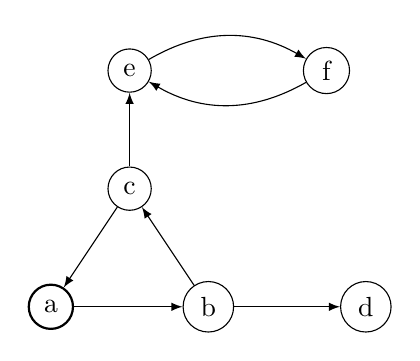
\begin{tikzpicture}
		\node (a)[circle, draw, thick]at (0,0)  {a};
		\node (b)[circle, draw]at (2,0)  {b};
		\node (c)[circle, draw]at (1,1.5)  {c};
		\node (d)[circle, draw]at (4,0)  {d};
		\node (e)[circle, draw]at (1,3)  {e};
		\node (f)[circle, draw]at (3.5,3)  {f};

		\draw [-latex](a)--(b);
		\draw [-latex](b)--(c);
		\draw [-latex](c)--(a);
		\draw [-latex](c)--(e);
		\draw [bend left, -latex](e)to(f);
		\draw [bend left, -latex](f)to(e);
		\draw [-latex](b)--(d);
	\end{tikzpicture}
\end{center}

Ad esempio potrei visitare come $ a - b -c - a - c - e - f - e - c -b -d-b-a $, il che corrisponderebbe ad un toposort di $ f - e - c - d - b - a $
\begin{center}
	\begin{tikzpicture}
		\node (a)[circle, draw] at (0,0)   {a};
		\node (b)[circle, draw] at (2,0)   {b};
		\node (d)[circle, draw] at (4,0)   {d};
		\node (c)[circle, draw] at (8,0)   {c};
		\node (e)[circle, draw] at (10,0)  {e};
		\node (f)[circle, draw] at (12,0)  {f};

		\draw [bend left, -latex](a) to(b);
		\draw [bend left,-latex](b)  to(c);
		\draw [bend left,-latex](c)  to(a);
		\draw [bend left,-latex](c)  to(e);
		\draw [bend left, -latex](e) to(f);
		\draw [bend left, -latex](f) to(e);
		\draw [bend left,-latex](b)  to(d);

		\node [draw, fit = (a) (b) (c), dashed]  {};
		\node [draw, fit = (e) (f), dashed]  {};
		\node [draw, fit = (d), dashed]  {};
	\end{tikzpicture}
\end{center}

\section{Hashing}
\subsection{Definizioni}
\begin{definizione}{Funzione hash}
	Dati:
	\begin{itemize}
		\item $ \mathcal{U} $: universo delle chiavi
		\item $ m $: dimensione della struttura dati che immagazzina i valori (\textit{hash-table})
		\item $ n $: numero di chiavi inserite
	\end{itemize}
	Una funzione hash è una funzione dall'universo delle chiavi $ \mathcal{U} $ ad un valore intero.
	\[
		h: \mathcal{U} \rightarrow \left\{0, 1, \dots, m-1\right\}
	\]
\end{definizione}
\begin{definizione}{Funzione hash perfetta}
	Una funzione hash è detta \textit{perfetta} se non genera collisioni:
	\[
		\forall k_1, k_2 \in \mathcal{U}: k_1 \neq k_2 \Rightarrow h(k_1) \neq h(k_2)
	\]
\end{definizione}
\begin{definizione}{Uniformità semplice}
	Una funzione di hash gode di uniformità semplice se applicandola su un valore estratto a caso la probabilità che finisca nell'i-esimo slot è di $ \frac{1}{m} $. In altri termini, ogni slot ha la stessa probabilità di essere selezionato dalla funzione di hash.
	\vskip3mm
	Formalmente
	\begin{itemize}
		\item Sia $P(k)$ la probabilità che una chiave $k$ sia inserita in tabella
		\item Sia $Q(i)$ la probabilità che una chiave finisca nella cella $i$
	\end{itemize}

	\[
		Q(i)=\sum_{k \in \mathcal{U}: h(k)=i} P(k)
	\]

	Una funzione hash $h$ gode di uniformità semplice se:

	\[
		\forall i \in[0, \ldots, m-1]: Q(i)=1 / m
	\]
\end{definizione}
\subsection{Funzioni hash stringhe}
Definiamo innanzitutto le seguenti operazioni:
\begin{itemize}
	\item $\operatorname{ord}(c):$ valore ordinale binario del carattere $c$ in qualche codifica
	\item bin $(k)$ : rappresentazione binaria della chiave $k$, concatenando i valori binari dei caratteri che lo compongono
	\item int(b): valore numerico associato al numero binario $b$
	\item $\operatorname{int}(k)=\operatorname{int}(\operatorname{bin}(k))$
\end{itemize}

\subsubsection{Estrazione}
Seleziono solo certi bit in una stringa, ad esempio ultimi. Facile collisione, vedi \verb|Coperto|, \verb|Roberto|
\subsubsection{Xor}
Divido la rappresentazione binaria della parola in gruppi di $ x $ bit, e ne eseguo lo \verb|xor| bit a bit (Il quale corrisponde alla somma)
\subsubsection{Metodo della divisione}
\begin{itemize}
	\item $ m $ dispari, meglio se numero primo
	\item $ H\left(k\right) = \operatorname{int}\left(k\right) \mod m $
\end{itemize}
\subsubsection{Metodo della moltiplicazione}
\begin{itemize}
	\item $m$ qualsiasi, meglio se potenza di 2
	\item $C$ costante reale, $0<C<1$
	\item Sia $i=\operatorname{int}(k)$
	\item $H(k)=\lfloor m \cdot(C \cdot i-\lfloor C \cdot i\rfloor)\rfloor$
\end{itemize}
Nota come di base questo coincida con prendere la parte decimale di $ C \cdot i $, ossia un numero "abbastanza casuale" compreso tra $ 0 $ e $ 1 $.
\vskip3mm
Implementativamente, si può calcolare $ H(k) $ in modo efficiente:
\begin{center}
	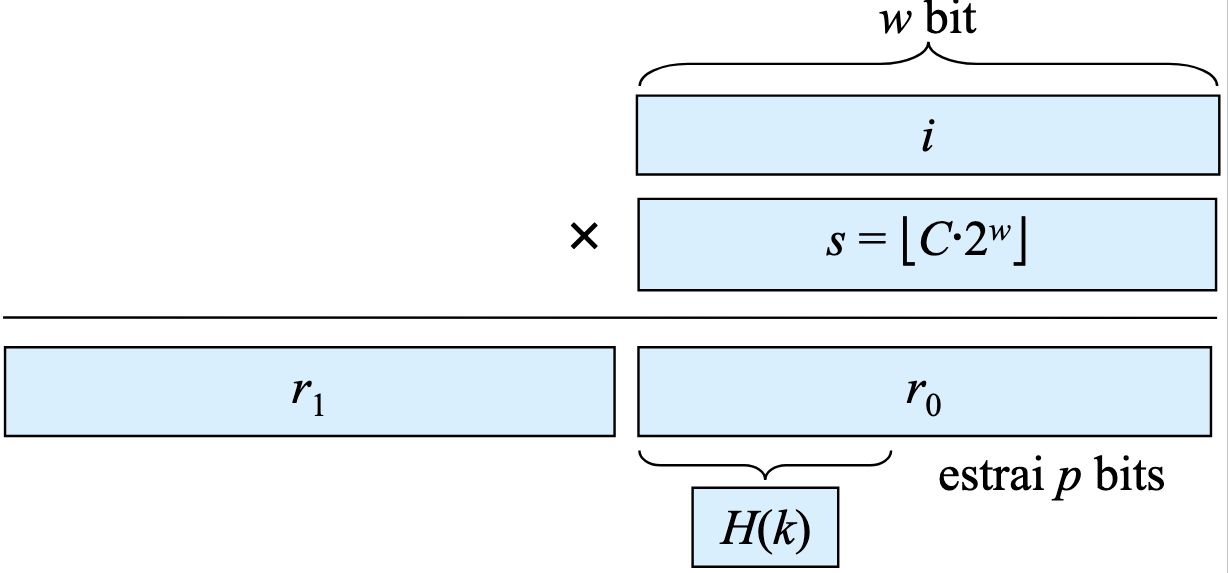
\includegraphics[width = 0.5\textwidth]{Images/knuth multiplication hash.png}
\end{center}
Questo coincide con
\begin{itemize}
	\item Considerare la costante $ C $ senza la virgola ($ s = C \cdot 2^{w} $, ossia shifto a sinistra di $ w $ bit)
	\item Eseguire la moltiplicazione
	\item I $ w $ bit più significativi contengono il risultato intero della moltiplicazione
	\item I $ w $ bit meno significativi contengono il risultato dopo la virgola
	\item Questo è vero perché dovrei shiftare nuovamente a destra il risultato, se avessi moltiplicato usando la virgola
\end{itemize}

\subsection{Liste di trabocco}
\vskip3mm
\begin{tabularx}{\textwidth}{lX}
	\toprule
	$n$             & Numero di chiavi memorizzati in tabella hash                                                                          \\
	\midrule
	$m$             & Capacità della tabella hash                                                                                           \\
	\midrule
	$\alpha=n / m $ & Fattore di carico                                                                                                     \\
	\midrule
	$I(\alpha)    $ & Numero medio di accessi alla tabella per la ricerca di una chiave non presente nella tabella (ricerca con insuccesso) \\
	\midrule
	$S(\alpha)    $ & Numero medio di accessi alla tabella per la ricerca di
	una chiave presente nella tabella (ricerca con successo)                                                                                \\
	\bottomrule
\end{tabularx}
\vskip3mm
In una hash map con liste di trabocco, il \textit{valore atteso} della lunghezza delle liste di trabocco è pari al \underline{fattore di carico} $ \alpha  = n / m $. In media quindi il costo è di
\begin{itemize}
	\item Ricerca senza successo: $ \theta \left(1\right) + \alpha  $
	\item Ricerca con successo: $ \theta \left(1\right) + \frac{\alpha}{2}  $
\end{itemize}
\subsection{Indirizzamento aperto}
Con l'indirizzamento aperto, ogni valore è salvato nello stesso vettore. Se lo slot scelto è già in uso, si tenta il prossimo
\vskip3mm
\begin{definizione}{Sequenza di ispezione}
	Una sequenza secondo la quale si esaminano gli slot
\end{definizione}
\begin{definizione}{Hashing uniforme}
	La situazione ideale prende il nome di hashing uniforme, in cui ogni
	chiave ha la stessa probabilità di avere come sequenza di ispezione
	una qualsiasi delle $ m! $ permutazioni di $ [0,\ldots  , m - 1] $
\end{definizione}
Abbiamo diverse possibilità nella scelta delle sequenze di ispezione:
\begin{itemize}
	\item \underline{Ispezione lineare}: $ H(k, i) = (H_1(k) +  h \cdot i) \mod m $
	      \begin{itemize}
		      \item Problema di \underline{agglomerazione primaria}: la cella dopo una sequenza di lunghezza $ i $ ha probabilità $ \frac{\left(i+1\right)}{m} $ di essere estratta
	      \end{itemize}
	\item \underline{Ispezione quadratica}: $ \left(H\left(k,i\right) = H_1\left(k\right) + h \cdot i^2  \right) \mod  m$
	\item \underline{Doppio hash:} $ H(k, i) = (H_1(k) + i \cdot H_2(k)) \mod m $
\end{itemize}
Nota che se utilizzi indirizzamento libero bisogna distinguere fra  inserimento e lookup. In particolare distinguiamo fra valori \verb|nil|, ossia mai inseriti e \verb|deleted|, ossia rimossi
\begin{itemize}
	\item Inserimento: scorriamo sequenza di ispezione ed inseriamo appena troviamo un valore \verb|nil| o \verb|deleted|
	\item Lookup: scorriamo finche incontriamo un valore \verb|nil| o il valore cercato. Sui valori \verb|deleted| andiamo avanti siccome potrebbe essere stato inserito più tardi nella sequenza di ispezione
\end{itemize}

\section{Divide et impera}
\subsection{Torri di hanoi}
Un algoritmo classico divide et impera è quello delle torri di hanoi. Si hanno 3 torri e si vuole spostare $ n $ dischi dalla prima all'ultima. Ogni disco non può essere impilato su un disco più piccolo
\vskip3mm
Chiamiamo le torri \verb|A, B, C|, a partire da SX. L'algoritmo procede così:
\begin{itemize}
	\item Sposto $ n-1 $ dischi da \verb|A| a \verb|B|
	\item Sposto il disco rimanente da \verb|A| a \verb|C|
	\item Sposto $ n-1 $ dischi rimasti da \verb|B| a \verb|C|
\end{itemize}
Ecco l'algoritmo in pseudo codice:


\begin{algoritmo} {Torri di hanoi}
	\begin{algorithm}[H]
		% \caption{hanoi tower algorithm}
		\SetKwFunction{Hanoi}{hanoi}
		\Fn{\Void \Hanoi{$n$, src, dest, middle}}{
			\If{$n = 1$}{
				\textbf{print} src $\rightarrow$ dest\;
			}
			\Else{
				\Hanoi{$n - 1$, src, middle, dest}\;
				\textbf{print} src $\rightarrow$ dest\;
				\Hanoi{$n - 1$, middle, dest, src}\;
			}
		}
	\end{algorithm}
\end{algoritmo}
\subsection{Algoritmo di Strassen}
L'idea è che possiamo esprimere il prodotto matriciale come segue, dividendo la matrice in 4:

\[
	A = \begin{bmatrix}
		A_{1,1} & A_{1,2} \\
		A_{2,1} & A_{2,2}
	\end{bmatrix} \quad
	B = \begin{bmatrix}
		B_{1,1} & B_{1,2} \\
		B_{2,1} & B_{2,2}
	\end{bmatrix}
\]


\[
	C = \begin{bmatrix}
		A_{1,1} \times B_{1,1} + A_{1,2} \times B_{2,1} & A_{1,1} \times B_{1,2} + A_{1,2} \times B_{2,2} \\
		A_{2,1} \times B_{1,1} + A_{2,2} \times B_{2,1} & A_{2,1} \times B_{1,2} + A_{2,2} \times B_{2,2}
	\end{bmatrix}
\]
Così facendo ottengo la ricorrenza:
\[
	T\left(n\right) = 8 T\left(\frac{n}{2}\right) + n^3
\]
In realtà posso eseguire i prodotti in modo intelligente, risparmiandone uno, ottenendo quindi
\[
	T\left(n\right) = 7 T\left(\frac{n}{2}\right) + n^2 \approx n^{2.81}
\]




%
% \subsection{Quicksort}\label{quicksort}
% L'algoritmo di quicksort procede cosi:
% \begin{itemize}
% 	\item Scegli un \textit{pivot} (un elemento a caso, di solito il primo)
% 	\item Per ogni valore nel vettore \verb|v|, metti alla sinistra del pivot i valori più piccoli del \verb|pivot| stesso, a destra i più grandi
% 	\item Ripeti ricorsivamente sui sottovettori a sx e dx del pivot
% \end{itemize}
%
% \subsection{Algoritmo di Strassen (moltiplicazione matriciale)}
% \textit{Strassen} fu il primo a scoprire che è possibile moltiplicare due matrici in $ \theta \left(n^{2.81}\right) $. Questo algoritmo sfrutta il fatto che si può dividere entrambe le matrici in 4
%
% Suddividiamo le matrici $n \times n$ in quattro matrici $n / 2 \times n / 2$
%
% \[
% 	A=\left[\begin{array}{ll}
% 			A_{1,1} & A_{1,2} \\
% 			A_{2,1} & A_{2,2}
% 		\end{array}\right] \quad B=\left[\begin{array}{ll}
% 			B_{1,1} & B_{1,2} \\
% 			B_{2,1} & B_{2,2}
% 		\end{array}\right]
% \]
%
%
% Calcolo prodotto matrice
%
% \[
% 	C=\left[\begin{array}{ll}
% 			A_{1,1} \times B_{1,1}+A_{1,2} \times B_{2,1} & A_{1,1} \times B_{1,2}+A_{1,2} \times B_{2,2} \\
% 			A_{2,1} \times B_{1,1}+A_{2,2} \times B_{2,1} & A_{2,1} \times B_{1,2}+A_{2,2} \times B_{2,2}
% 		\end{array}\right]
% \]
%
%
% Siccome dobbiamo eseguire 8 prodotti matriciali, l'equazione di ricorrenza e la seguente:
%
% \[
% 	T(n)= \begin{cases}1 & n=1 \\ 8 T(n / 2)+n^2 & n>1\end{cases}
% \]
% Tuttavia, se salviamo dei valori intermedi, riusciamo a risparmiarci un prodotto:
% \[
% 	\begin{aligned}
% 		 & X_1=\left(A_{11}+A_{22}\right) \times\left(B_{11}+B_{22}\right)   \\
% 		 & X_2=\left(A_{21}+A_{22}\right) \times B_{11}                      \\
% 		 & X_3=A_{11} \times\left(B_{12}-B_{22}\right)                       \\
% 		 & X_4=A_{22} \times\left(B_{21}-B_{11}\right)                       \\
% 		 & X_5=\left(A_{11}+A_{12}\right) \times B_{22}                      \\
% 		 & X_6=\left(A_{21}-A_{11}\right) \times\left(B_{11}+B_{12}\right)   \\
% 		 & X_7=\left(A_{12}-A_{22}\right) \times\left(B_{21}+B_{22}\right) .
% 	\end{aligned}
% \]
%
%
% Calcolo matrice finale
%
% \[
% 	C=\left[\begin{array}{cc}
% 			X_1+X_4-X_5+X_7 & X_3+X_5         \\
% 			X_2+X_4         & X_1+X_3-X_2+X_6
% 		\end{array}\right]
% \]
%
% Otteniamo dunque una complessità inferiore pari a:
% \[
% 	\begin{aligned}
% 		 & T(n)= \begin{cases}1              & n=1 \\
%              7 T(n / 2)+n^2 & n>1\end{cases}                                   \\
% 		 & T(n)=\Theta\left(n^{\log _2 7}\right) \approx \Theta\left(n^{2.81}\right)
% 	\end{aligned}
% \]
% \subsection{Gap (problema esempio)}
% Supponiamo di voler risolvere il seguente problema:
% \vskip3mm
% \hrule
% \vskip3mm
% In un array un gap è un suo indice $ i $ tale per cui:
% \[
% 	v\left[i\right] > v\left[i-1\right]
% \]
% Sapendo che in un vettore di lunghezza $ n $ $ v\left[0\right] < v\left[n-1\right] $, trovare un algoritmo che restituisca l'indice a cui si trova il gap.
% \vskip3mm
% \hrule
% \vskip3mm
% Si dimostra per induzione o per assurdo che il gap esiste. Per trovarlo tramite un algoritmo posso sfruttare il divide et impera come segue:
% \vskip3mm
% \begin{algoritmo}{Gap}
% 	\begin{algorithm}[H]
% 		\DontPrintSemicolon
% 		\SetKwFunction{GapRec}{gapRec}
% 		\Fn{\Void \GapRec{$\Int[]\ V$, $\Int\ i$, $\Int\ j$}}{
% 			\If{$j == i + 1$}{
% 				\Return $j$\;
% 			}
% 			$m \leftarrow \lfloor (i + j) / 2 \rfloor$\;
% 			\If{$V[m] < V[j]$}{
% 				\Return \GapRec{$V$, $m$, $j$}\;
% 			}
% 			\Else{
% 				\Return \GapRec{$V$, $i$, $m$}\;
% 			}
% 		}
% 		\caption{Recursive Gap Finder}
% 	\end{algorithm}
% \end{algoritmo}
% \section{Strutture dati speciali}
% \subsection{Priority queue (heap)}
% Per ripristinare le proprie proprietà di un heap una volta inserito un elemento possiamo usare quanto segue. La funzione assume che $ i $ sia la radice e che i due sottoalberi dtro e sinistro rispettino già le proprietà del \textit{max-min-heap}
% \vskip3mm
% \begin{algoritmo}{Max headp restore}
% 	\begin{algorithm}[H]
% 		\caption{Restore max-heap starting from index $i$}
% 		\SetKwFunction{MaxHeapRestore}{maxHeapRestore}
% 		\Fn{\Void \MaxHeapRestore{$\Item[]\ A$, $\Int\ i$, $\Int\ dim$}}{
% 			$max \gets i$\;
% 			\If{$l(i) \leq dim$ \And $A[l(i)] > A[max]$}{
% 				$max \gets l(i)$\;
% 			}
% 			\If{$r(i) \leq dim$ \And $A[r(i)] > A[max]$}{
% 				$max \gets r(i)$\;
% 			}
% 			\If{$i \neq max$}{
% 				swap($A$, $i$, $max$)\;
% 				\MaxHeapRestore{$A$, $max$, $dim$}\;
% 			}
% 		}
% 	\end{algorithm}
% \end{algoritmo}
% \vskip3mm
% Complessità: $ O \left(\log n\right) $
% \vskip3mm
% Per costruire un heap a partire da un array posso utilizzare semplicemente il seguente algoritmo:
% \vskip3mm
% \begin{algoritmo}{Max heap build}
% 	\begin{algorithm}[H]
% 		\caption{Buil max-min-heap starting from array}
% 		\SetKwFunction{MaxHeapRestore}{maxHeapRestore}
% 		\SetKwFunction{HeapBuild}{heapBuild}
% 		\Fn{\Void \HeapBuild{$\Item[]\ A$, $\Int\ dim$}}{
% 			\For{$i \gets \lfloor dim / 2 \rfloor$ \KwTo $1$}{
% 				\MaxHeapRestore{$A$, $i$, $dim$}\;
% 			}
% 		}
% 	\end{algorithm}
% \end{algoritmo}
% Devo partire da $ \left\lfloor \frac{dim}{2} \right\rfloor $ altrimenti partirei dalla radice dell'albero. $ \left\lfloor \frac{dim}{2} \right\rfloor $ è l'indice dell'ultimo \underline{nodo interno} dell'albero
% \vskip3mm
% Complessità: $ O  \left(n\right) $
% \vskip3mm
% Posso sfruttare l'heap anche per fare sorting di un array come segue:
% \vskip3mm
% \begin{algoritmo}{Heap sort}
% 	\begin{algorithm}[H]
% 		\caption{Sort array using a heap}
% 		\SetKwFunction{HeapSort}{heapSort}
% 		\SetKwFunction{HeapBuild}{heapBuild}
% 		\SetKwFunction{Swap}{swap}
% 		\SetKwFunction{HeapRestore}{heapRestore}
% 		\Fn{\Void \HeapSort{$\Item[]\ A$, $\Int\ dim$}}{
% 			\HeapBuild($A$, $dim$)\;
% 			\For{$i = dim$ \Downto $1$}{
% 				\Swap($A$, $1$, $i$)\;
% 				\HeapRestore($A$, $1$, $i - 1$)\;
% 			}
% 		}
% 	\end{algorithm}
% \end{algoritmo}
% \vskip3mm
% Complessità: $ \Theta \left(n \log n\right) $
% \subsection{Merge find set}
% Se è necessario tenere traccia di un un insieme di insiemi disgiunti (ad esempio le componenti connesse di un grafo), ci possiamo servire di un merge find set. Questa strutture ci permette di unire le diverse componenti in maniera efficace
%
% \begin{figure}[H]
% 	\begin{subfigure}[b]{0.5\textwidth}
% 		\centering
% 		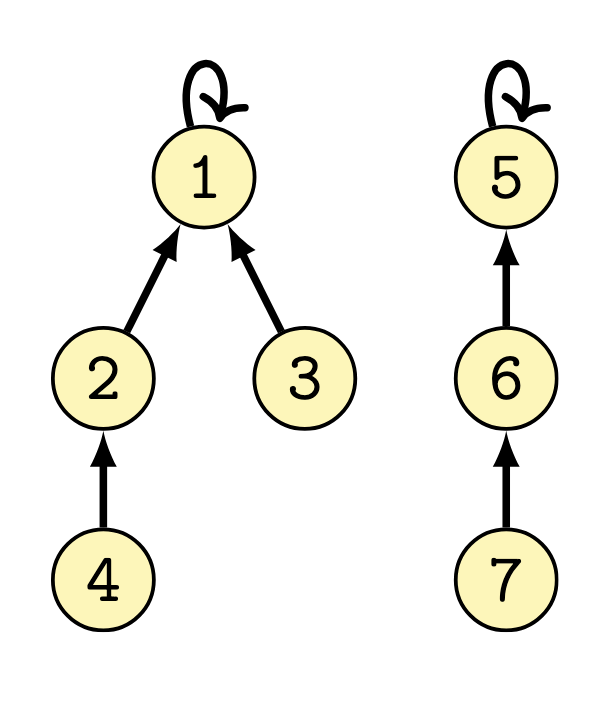
\includegraphics[width=0.2\textwidth]{Images/mf tree.png}
% 		\caption{Rappresentazione tramite alberi}
% 	\end{subfigure}
% 	%
% 	\begin{subfigure}[b]{0.5\textwidth}
% 		\centering
% 		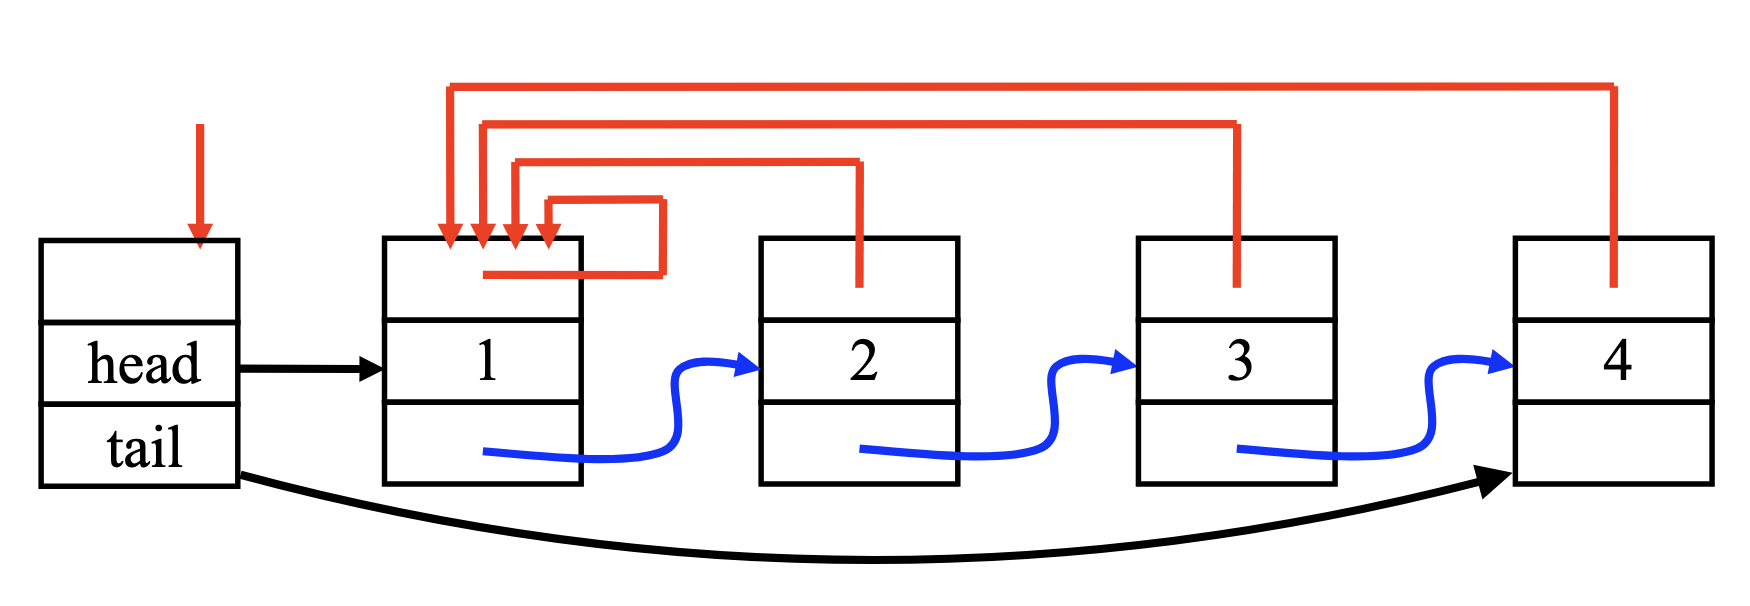
\includegraphics[width=0.6\textwidth]{Images/mf list.png}
% 		\caption{Rappresentazione tramite lista}
% 	\end{subfigure}
% \end{figure}
% \subsubsection{Euristiche}
% Per mantenere efficiente ogni operazione si possono applicare delle euristiche:
% \begin{itemize}
% 	\item Euristica sul peso (liste): in \verb|merge()| attacco lista corta a lista lunga. Garantisce che \verb|merge|() abbia complessità $ O\left(\log n\right) $
% 	\item Euristica sul rango (alberi): in \verb|merge()| attacco albero con rango minore a quello con rango maggiore. Questo garantische che l'altezza di ogni albero sia al più $ \log n $
% 	\item Euristica di compressione dei cammini: quando eseguo \verb|find|, attacco nodo direttamente alla radice dell'albero. Questo ci permette di utilizzare l'analisi ammortizzata e ridurre la complessità
% \end{itemize}
% In particolare ottengo che applicando l'euristica sul rango e sulla compressione dei cammini la complessità finale è di
% \[
% 	O \left(m * \alpha \left(n\right)\right)
% \]
% dove $ \alpha\left(n\right)  $ è la \href{https://it.wikipedia.org/wiki/Funzione_di_Ackermann}{\textit{funzione inversa di Ackermann}}, che è praticamente costante (per $ n < 2^{65536},  \alpha \left(N\right) < 5$)
%
% \subsubsection{Riassumendo}
% \begin{center}
% 	\begin{tabular}{|l|l|l|}
% 		\hline Algoritmo                                    & find ()     & merge ()      \\
% 		\hline \hline
% 		Liste                                               & $O(1)$      & $O(n)$        \\
% 		\hline Alberi                                       & $O(n)$      & $O(1)^{+}$    \\
% 		\hline Liste + Euristica sul peso                   & $O(1)$      & $O(\log n)^*$ \\
% 		\hline Alberi + Euristica sul rango                 & $O(\log n)$ & $O(1)^{+}$    \\
% 		\hline
% 		Alberi + Euristica sul rango + Compressione cammini & $O(1)^*$    & $O(1)$        \\
% 		\hline
% 	\end{tabular}
% \end{center}









\section{Strutture dati speciali}
\subsection{Heap}\label{heap}
Abbiamo bisogno di 2 funzioni:
\begin{itemize}
	\item \verb|heapbuild|: costruisce un heap
	\item \verb|heaprestore|: dato un heap con una possibile violazione nella radice, ripristina le proprietà di min/max heap
\end{itemize}
\subsubsection{Heap restore}
Posso avere una violazione nella radice di un heap. Controllo il nodo root \verb|r|
\begin{itemize}
	\item Se $ r.val $ è maggiore di entrambi i figli non violo nulla
	\item Se \verb|r.val| non è maggiore di entrambi i figli allora lo scambio con il figlio maggiore. Chiamo ricorsivamente sul sottoalbero del figlio maggiore (l'altro sottoalbero rimane inalterato)
\end{itemize}
\subsubsection{Heap build}
Innanzitutto nota che

\begin{itemize}
	\item Sia $A[1 \ldots n]$ un vettore da ordinare
	\item Tutti i nodi $A[\lfloor n/2 \rfloor + 1 \ldots n]$ sono foglie
	      dell'albero e quindi heap contenenti 1 elemento
\end{itemize}

\begin{center}
	\begin{forest}
		for tree={draw, circle, align=center, grow = -90}
		[1, thick
			[2
					[4
							[8, thick]
							[9, thick]
					]
					[5
							[10, thick]
							[11, thick]
					]
			]
			[3
					[6
							[12, thick]
					]
					[7, thick]
			]
		]
	\end{forest}
\end{center}

Il fatto che gli ultimi $ \frac{n}{2} $ elementi dell'array siano foglie è dato dal fatto che dato un nodo di indice i allora $ \frac{i}{2} $ è suo padre
Dunque, la procedura \texttt{heapBuild()}
\begin{itemize}
	\item attraversa i restanti nodi dell'albero, a partire
	      da $\lfloor n/2 \rfloor$ fino ad $1$
	\item esegue \texttt{maxHeapRestore()} su ognuno di essi
\end{itemize}
\begin{algoritmo}{Headp build}
	\begin{algorithm}[H]
		\SetKwFunction{FHeapBuild}{heapBuild}
		\SetKw{DownTo}{downto}
		\Fn{\FHeapBuild{\Item [] $A$, \Int $n$}}{
			\For{$i = \lfloor n/2 \rfloor$ \DownTo $1$ }{
				maxHeapRestore($A$, $i$, $n$)\;
			}
		}
	\end{algorithm}
\end{algoritmo}

Verrebbe naturale affermare che la complessità è $ \Theta\left(n \log\left(n\right)\right) $, ma è in realtà $ \Theta \left(n\right) $. Ora l'idea è di dividere per livelli il calcolo della complessità. In particolare dividiamo i nodi in base alla loro altezza
\vskip3mm
\begin{center}
	\begin{forest}
		for tree={text=white, draw, circle, align=center, grow = -90, scale=0.7}
		[1, fill=mutedpurple!50
		[2, fill=mutedpurple!50
		[4, fill=mutedred!50
		[8, thick, fill=mutedblue!50
		[16, thick, fill=black!50]
		[17, thick, fill=black!50]
		]
		[9, thick, fill=mutedblue!50
		[18, thick, fill=black!50]
		[19, thick, fill=black!50]
		]
		]
		[5, fill=mutedred!50
		[10, thick, fill=mutedblue!50
		[20, thick, fill=black!50]
		[21, thick, fill=black!50]
		]
		[11, thick, fill=mutedblue!50
		[22, thick, fill=black!50]
		[23, thick, fill=black!50]
		]
		]
		]
		[3, fill=mutedred!50
		[6, fill=mutedred!50
		[12, thick, fill=mutedblue!50
		[24, thick, fill=black!50]
		[25, thick, fill=black!50]
		]
		[13, thick, fill=mutedblue!50
		[26, thick, fill=black!50]
		[27, thick, fill=black!50]
		]
		]
		[7, thick, fill=mutedblue!50
		[14, thick, fill=mutedblue!50
		[28, thick, fill=black!50]
		]
		[15, thick, fill=black!50]
		]
		]
		]
	\end{forest}
\end{center}
\vskip3mm
Chiamo $ h $ l'altezza dell'albero. Nota che per il livello $ i $, a partire dall'ultimo (quello più in basso), abbiamo $ \frac{n}{2} $ nodi e per ognuno di essi dobbiamo eseguire al più 1 operazione. Più in generale:
\begin{center}
	\begin{tabular}{c c c}
		\toprule
		Livello (dal basso) & Numero operazioni & Numero di nodi  \\
		\midrule
		1                   & $ 1 $             & $ n / 2 $       \\
		2                   & $ 2 $             & $ n / 4 $       \\
		$ \vdots $          & $ \vdots $        & $ \vdots $      \\
		i                   & i                 & $ n / (2^{i}) $ \\
		\bottomrule
	\end{tabular}
\end{center}
Quindi il costo totale è dato da:
\begin{align*}
	T\left(n\right) = \sum_{i=1}^{\left\lfloor \log \left(n\right) \right\rfloor} \frac{n}{2^i}\cdot i = n \sum_{i=1}^{\left\lfloor \log \left(n\right) \right\rfloor} \left(\frac{1}{2}\right)^{i} i \le n \sum_{i=1}^{\infty} \left(\frac{1}{2}\right)^{i} i
\end{align*}
Questa è una successione geometrica:
\[
	\sum_{k=1}^{\infty} k a^{k} = \frac{a}{\left(1 - a\right)^{2}}
\]
dunque
\[
	T\left(n\right) \le n \sum_{i=1}^{\infty} \left(\frac{1}{2}\right)^{i} i = n \cdot \frac{1 / 2}{\left(1 / 2 \right)^{2}} = 2 n =  O\left(n\right)
\]
\subsubsection{Heap insert}\label{heap insert}
Semplicemente prende un elemento e lo mette nell'ultima posizione dell'array, quindi l'ultimo figlio a destra nell'ultimo livello. Ricorsivamente chiama heap restore sul parent
\subsubsection{Heap remove min}
Swappa l'elemento nella root e l'ultimo elemento a destra nell'ultimo livello. Chiama \verb|heap restore| sulla root

\subsection{Priority queue}
Una priority queue usa un heap come descritto in sezione \ref{heap} per fornire accesso in tempo costante all'elemento maggiore/minore.

\subsubsection{Decremento/incremento priorità}
\begin{itemize}
	\item Se è una minqueue e la prirorità aumenta, oppure ho una maxqueue e la priorità diminuisce è sufficiente chiamare \verb|heap_restore| sul nodo coinvolto
	\item Se è una minqueue e la priorità diminuisce, oppure ho una maxqueue e la priorità aumenta, devo chiamare ricorsivamente \verb|heaprestore| su padre, come nell'inserimento descritto in sezione \ref{heap insert}
\end{itemize}
\begin{center}
	\begin{tabular}{l l l}
		\toprule
		Tipo coda & incremento  & decremento  \\
		\midrule
		minqueue  & heaprestore & recurse up  \\
		maxqueue  & recurse up  & heaprestore \\
		\bottomrule
	\end{tabular}
\end{center}

\subsection{Merge find set}
\subsubsection{Realizzazione con liste}
\begin{itemize}
	\item Il primo elemento della lista contiene il rappresentante della componente
	\item Ogni elemento della lista contiene un puntatore al rappresentante
	\item Per unire le liste
\end{itemize}
Dunque \verb|find()| ha complessità $ O(1) $ e \verb|merge()| ha complessità $ O(n) $. Tuttavia su $ n $ operazioni, \verb|merge()| ha complessità ammortizzata di $ O\left(n\right) $
\subsubsection{Realizzazione con alberi}
\begin{itemize}
	\item Il rappresentante è la radice. La radice ha un self loop
	\item Per trovare rappresentante risalgo fino a radice
	\item Per fare merge attacco radice di un albero a radice dell'altro
\end{itemize}
Dunque \verb|merge()| ha complessità $ O(1) $ e \verb|find()| ha complessità $ O(n) $. Si possono usare euristiche per ridurre la complessità di find a $ O\left(\log n\right) $
\subsubsection{Euristica sul peso (liste)}
Attacco sempre lista più corta a lista più lunga. Complessità di \verb|merge| diventa $ O\left(\log \left(n\right)\right) $
\subsubsection{Euristica sul rango (alberi)}
Attacco sempre albero con altezza massima minore a quello con altezza massima maggiore. Dunque:
\begin{itemize}
	\item Se \verb|rango(t1) == rango(t2)| allora rango aumenta di 1
	\item Il rango rimane uguale a \verb|max(rango(t1), rango(t2))| se \verb|rango(t1) !=  rango(t2)|
\end{itemize}
Quindi visto che posso effettuare al massimo $ \log \left(n\right) $ operazioni di merge, il rango massimo è $ \log \left(n\right) $. Formalmente procedo per induzione e dimostro che $ n > 2^{\operatorname{rank}} $, dove \verb|rank| è l'altezza massima dell'albero:

\begin{itemize}
	\item \sfblue{Caso base}: nel nodo singolo $ \operatorname{rank} = 0 \rightarrow 1 \ge 2^{0}$
	\item \sfblue{Induzione caso 1:} $\operatorname{rank}[x] > \operatorname{rank}[y]$
	      \begin{itemize}
		      \item Il rango finale è pari a $\operatorname{rank}[x]$

		      \item Per induzione, il numero di nodi è:
		            \[
			            n \geq 2^{\operatorname{rank}[x]} + 2^{\operatorname{rank}[y]} \ge 2^{\operatorname{rank}[x]}
		            \]
	      \end{itemize}

	\item \sfblue{Induzione caso 2:} $\operatorname{rank}[x] = \operatorname{rank}[y]$
	      \begin{itemize}
		      \item Il rango finale è pari a $\operatorname{rank}[x] + 1$

		      \item Per induzione, il numero di nodi è:
		            \[
			            n \geq 2^{\operatorname{rank}[x]} + 2^{\operatorname{rank}[y]} \ge \operatorname{rank}[x] = 2 \cdot 2^{\operatorname{rank}[x]} \ge 2^{\operatorname{rank}[x] + 1}
		            \]
		            come volevasi dimostrare
	      \end{itemize}
\end{itemize}


\subsubsection{Euristica di compressione dei cammini}
L'idea è di appiattire l'albero attaccando i nodi direttamente alla radice, facendo si che \verb|find()| abbia complessità costante

\begin{center}
	\begin{tabular}{l l l}
		\toprule
		\sfblue{Algoritmo}           & \sfblue{find()} & \sfblue{merge()} \\
		\midrule
		Liste                        & $O(1)$          & $O(n)$           \\
		Alberi                       & $O(n)$          & $O(1)^+$         \\
		Liste + euristica sul peso   & $O(1)$          & $O(\log n)^*$    \\
		Alberi + euristica sul rango & $O(\log n)$     & $O(1)^+$         \\

		\makecell[l]{Alberi + euristica sul rango +                       \\ compressione cammini} & $O(1)^*$        & $O(1)$           \\
		\bottomrule
	\end{tabular}
\end{center}


\section{Programmazione dinamica}
\subsection{Donimo}
Quanti modi ho di disporre tasselle di domino in una scacchiera $ 2 \times n $?

\subsubsection{Soluzione}
\begin{itemize}
	\item Salvo in $ dp\left[i\right] $ il numero di combinazioni che ci sono per un rettangolo $ 2 \times i $
	\item Ho due opzioni:
	      \begin{itemize}
		      \item Metto 2 tessere in orizzontale, allora $ dp\left[i\right] = dp\left[i-2\right] $
		      \item Metto 1 tessera in verticale, allora $ dp\left[i\right] = dp\left[i-1\right] $
	      \end{itemize}
	\item Quindi $ dp\left[i\right] = dp\left[i-1\right] + dp\left[i-2\right] $
	\item La soluzione è $ \operatorname{Fib}\left(n\right) $
\end{itemize}
\subsection{Hateville}
Ho un vettore di prezzi. Se prendo un prezzo $ v\left[i\right] $ non posso prendere $ v\left[i-1\right] $ e $ v\left[i+1\right] $. Trova prezzo massimo

\subsubsection{Soluzione}
\begin{itemize}
	\item Salvo in $ dp\left[i\right] $ il prezzo massimo che posso ottenere con i vicini $ \le i $
	\item Ho due opzioni:
	      \begin{itemize}
		      \item Non prendo $ v\left[i\right] $, allora il prezzo è $ dp\left[i-1\right] $
		      \item Prendo $ v\left[i\right] $, allora il prezzo è $ dp\left[i-1\right] + v\left[i\right] $
	      \end{itemize}
\end{itemize}
\subsection{Zaino}\label{zaino}
Zaino ha capacità $ C $, ho $ n $ pezzi di peso $ w\left[i\right] $ e profitto $ p\left[i\right] $. Trova profitto massimo

\subsubsection{Soluzione}
\begin{itemize}
	\item Crea matrice $ n \times C $ in cui si salva $ dp\left[i\right]\left[j\right] $ il profitto massimo che si può ottenere con i pezzi $ \le i $ e capacità $ \le j $
	\item Ho due opzioni:
	      \begin{itemize}
		      \item Prendo pezzo $ \left(i,j\right) $, allora il prezzo migliore è $ dp\left[i-1\right]\left[j - w\left[i\right]\right] + p\left[i\right] $
		      \item Non lo prendo, allora il prezzo è $ dp\left[i-1\right]\left[j\right] $
	      \end{itemize}
	\item Posso ottimizzare lo spazio tenendo salvato solo due righe della matrice, la $ i $ e la $ i-1 $
\end{itemize}
\subsection{Zaino umbound}
Vedi \hyperref[zaino]{zaino}, solo che non c'è limite al numero di oggetti che uno puo prendere

\subsubsection{Soluzione}
\begin{itemize}
	\item Vettore $ dp $ in cui salvo in $ i $ il profitto massimo per uno zaino grande $ i $
	\item Per ogni peso item $ x $, il profitto massimo è $ p\left[x\right] + dp\left[i - w\left[x\right]\right] $
	\item $ dp\left[i\right] $ è il massimo fra tutti i valori trovati al punto 2
\end{itemize}
\subsection{LCS}
Date due stringhe $ U $ e $ T $, trova la \underline{sottosequenza} massimale. Una sottosequenza è una stringa che si ottiene da un'altra selezionandone solo alcuni caratteri (non necessariamente contigui, ma mantenendone l'ordine).
\subsubsection{Soluzione}
\begin{itemize}
	\item Tabella $ dp $ con $ U $ su un lato e $ T $ sull'altro. In $ dp\left[i\right]\left[j\right] $ salvo la lunghezza della $ LCS $ fra la sottostringa $ U\left[0,i\right] $ e $ T\left[0, j\right] $
	\item Ho due opzioni:
	      \begin{itemize}
		      \item $ U\left[i\right] = T[j] $, allora $ dp\left[i\right]\left[j\right] = dp\left[i-1\right]\left[j-1\right] +1 $ (aggiungo un carattere alla LCS più corta di 1)
		      \item $  U\left[i\right] \neq T[j] $  allora $ dp\left[i\right]\left[j\right] = \operatorname{max}\left(dp\left[i-1\right]\left[j\right], dp\left[i\right]\left[j-1\right]\right) $. Vedi immagine
	      \end{itemize}
\end{itemize}

\begin{center}
	\begin{tikzpicture}[scale=0.7]
		\draw [fill=mutedgreen!50](6, 0)rectangle ++ (2,1);
		\draw (0,0)grid(8,1);

		\draw [fill=mutedred!50](6, -3)rectangle ++ (4,1);
		\draw (0,-3)grid(10,-2);

		\begin{scope}[shift={(0.5,0.5)}]
			\node at (-1, 0) {$ U $};

			\node (1) at (0,0)  {a};
			\node (2) at (1,0)  {u};
			\node (3) at (2,0)  {t};
			\node (4) at (3,0)  {s};
			\node (5) at (4,0)  {s};
			\node (6) at (5,0)  {g};
			\node (7) at (6,0)  {n};
			\node (18) at (7,0)  {k};
			\node [anchor = south] at (7,0.5)  {$ i $};

			\node at (-1, -3) {$ V $};

			\node (8)  at (0,-3)  {w};
			\node (9)  at (1,-3)  {a};
			\node (10) at (2,-3)  {t};
			\node (11) at (3,-3)  {f};
			\node (12) at (4,-3)  {x};
			\node (13) at (5,-3)  {m};
			\node (14) at (6,-3)  {g};
			\node (15) at (7,-3)  {o};
			\node (16) at (8,-3)  {i};
			\node (17) at (9,-3)  {m};
			\node [anchor = south] at (6,-2.5)  {$ j $};
			% \node (15) at (7,-3)  {o};
			% \node (16) at (8,-3)  {i};

		\end{scope}

		\node (lcs)[circle] at (2,-1) {lcs};

		\draw (lcs)edge(1.south) edge (3.south) edge(6.south);
		\draw (lcs)edge(9.north) edge (10.north) edge(14.north);

	\end{tikzpicture}
\end{center}

Per migliorare la soluzione, se i caratteri sono diversi, devo aggiungere un carattere che sia nell'insieme dei caratteri dopo l'ultimo carattere comune. Quindi ho che
\begin{itemize}
	\item A $ T $, devo aggiungere un carattere che appartiene all'insieme rosso
	\item A $ U $, devo aggiungere un carattere che appartiene all'insieme verde
\end{itemize}
Chiaramente la cosa è asimmetrica, per questo devo controllare $ dp\left[i-1\right]\left[j\right] $ e $ dp\left[i\right]\left[j-1\right] $
\vskip3mm
\sfblue{Dimostrazione formale}: dobbiamo dimostrare che date due parole $ U \left(u_1,\ldots ,u_i\right) $ e $ V\left(v_1 , \ldots v_j\right) $ e $ X \left(x_1 , \ldots x_k\right) $ allora
\begin{itemize}
	\item Se $ u_i = v_j $  allora
	      \begin{gather*}
		      u_i = v_j = x_k \\
		      X\left(K-1\right) \in \mathcal{LCS}\left(U\left(i-1\right), V\left(j-1\right)\right)
	      \end{gather*}
	\item Se $ u_i \neq v_j $ e $ x_k \neq  u_i $ allora
	      \[
		      X \in \mathcal{LCS}\left(U\left(i-1\right), V \right)
	      \]
	\item Se $ u_i \neq v_j $ e $ x_k \neq  v_j $ allora
	      \[
		      X \in \mathcal{LCS}\left(U, V\left(j-1\right) \right)
	      \]
\end{itemize}

\begin{minipage}[t]{0.48\textwidth}
	\begin{center}
		\begin{tikzpicture}[scale=0.7]
			\draw (0,0)grid(8,1);
			\draw [fill=mutedgreen!50](7, 0)rectangle ++ (1,1);

			\draw (0,-3)grid(7,-2);
			\draw [fill=mutedred!50](6, -3)rectangle ++ (1,1);

			\begin{scope}[shift={(0.5,0.5)}]
				\node at (-1, 0) {$ U $};

				\node (1) at (0,0)  {a};
				\node (2) at (1,0)  {u};
				\node (3) at (2,0)  {t};
				\node (4) at (3,0)  {s};
				\node (5) at (4,0)  {s};
				\node (6) at (5,0)  {g};
				\node (7) at (6,0)  {n};
				\node (17) at (7,0)  {k};
				\node [anchor = south] at (7,0.5)  {$ i $};

				\node at (-1, -3) {$ V $};

				\node (8)  at (0,-3)  {w};
				\node (9)  at (1,-3)  {a};
				\node (10) at (2,-3)  {t};
				\node (11) at (3,-3)  {f};
				\node (12) at (4,-3)  {x};
				\node (13) at (5,-3)  {m};
				\node (14) at (6,-3)  {g};
				\node [anchor = south] at (6,-2.5)  {$ j $};
				% \node (15) at (7,-3)  {o};
				% \node (16) at (8,-3)  {i};

			\end{scope}

			\node (lcs)[circle] at (2,-1) {lcs};

			\draw (lcs)edge(1.south) edge (3.south) edge(6.south);
			\draw (lcs)edge(9.north) edge (10.north) edge(14.north);

		\end{tikzpicture}
	\end{center}
\end{minipage}
%
\begin{minipage}[t]{0.48\textwidth}
	\begin{center}
		\begin{tikzpicture}[scale=0.7]

			\draw (0,0)grid(6,1);
			\draw [fill=mutedblue!50](5, 0)rectangle(6,1);

			\draw (0,-3)grid(7,-2);
			\draw [fill=mutedblue!50](6, -3)rectangle(7,-2);

			\begin{scope}[shift={(0.5,0.5)}]
				\node at (-1, 0) {$ U $};

				\node (1) at (0,0)  {a};
				\node (2) at (1,0)  {u};
				\node (3) at (2,0)  {t};
				\node (4) at (3,0)  {s};
				\node (5) at (4,0)  {s};
				\node (6) at (5,0)  {g};
				\node [anchor = south] at (5,0.5)  {$ i $};

				\node at (-1, -3) {$ V $};

				\node (8)  at (0,-3)  {w};
				\node (9)  at (1,-3)  {a};
				\node (10) at (2,-3)  {t};
				\node (11) at (3,-3)  {f};
				\node (12) at (4,-3)  {x};
				\node (13) at (5,-3)  {m};
				\node (14) at (6,-3)  {g};
				\node [anchor = south] at (6,-2.5)  {$ j $};
				% \node (15) at (7,-3)  {o};
				% \node (16) at (8,-3)  {i};

			\end{scope}

			\node (lcs)[circle] at (2,-1) {lcs};

			\draw (lcs)edge(1.south) edge (3.south) edge(6.south);
			\draw (lcs)edge(9.north) edge (10.north) edge(14.north);

		\end{tikzpicture}
	\end{center}
\end{minipage}


\subsection{Occorrenza k approssimata}
Data una stringa $ t $ e una $ p $, diciamo che la distanza $ k $ di $ p $ da $ t $ è il numero \underline{minimo} di \textit{inserimenti, eliminazioni e scambi} che dobbiamo fare in $ t $ per far si che $ t == p $.
\[
	t = \text{ "scempio" }, \quad p = \text{ esempio } \rightarrow k = 2
\]
ad esempio, scambiando la "s" e "c" di \textit{scempio} in "e" ed "s" rispettivamente
\vskip3mm
Il problma sta nel trovare in un testo $ t $, la distanza minima di un pattern $ p $ da una sua qualsiasi sottostringa.
\vskip3mm
Ciò equivale a trovare quanti inserimenti, rimozioni e scambi devo fare \underline{nel testo} per far si che il pattern diventi una sua sottostringa
\subsubsection{Soluzione}
\begin{itemize}
	\item Inizializza matrice che ha $ p $ in verticale e $ t $ in orizzontale
	\item In $ dp\left[i\right]\left[j\right] $ si salva \textit{il minor valore di k per far si che $ p\left[0, i\right] $ sia sottostringa di $ t\left[0, j\right] $ che finisca in $ j $}
	\item Se $ p\left[i\right] == t\left[j\right] $ allora non serviranno altre mosse per riportare la soluzione di $ dp\left[i-1\right]\left[j-1\right] $ alla soluzione corrente
	\item Se $ p\left[i\right] \neq  t\left[j\right] $  allora posso fare 3 cose:
\end{itemize}

\begin{center}
	% 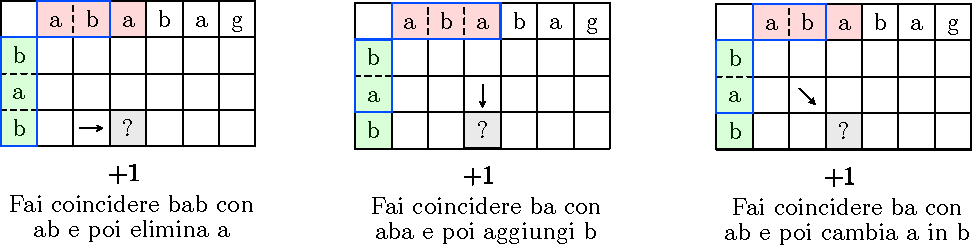
\includegraphics{Images/K approx.pdf }
	\begin{tikzpicture}[scale=0.6]

		\begin{scope}
			\draw [fill=mutedred!50](1,4)rectangle(4,3);
			\draw [fill=mutedgreen!50](0,0)rectangle(1,3);

			\draw (0,0)grid(7,4);

			\draw [thick, mutedblue](0,0)rectangle(1,3);
			\draw [thick, mutedblue](1,4)rectangle(3,3);

			\begin{scope}[shift={(0.5,0.5)}]
				\node at (0,2){b};
				\node at (0,1){a};
				\node at (0,0){b};

				\node at (1,3){a};
				\node at (2,3){b};
				\node at (3,3){a};
				\node at (4,3){b};
				\node at (5,3){a};
				\node at (6,3){g};

				\node at (3,0){?};
				\node at (2,0){$ \rightarrow $};

				% \node at[3,0] {Fai coincidere bab con ab e poi elimina a};
				\node at (3,-1) {+1};
				\node [align = center] at (3,-2) {Fai coincidere bab con ab\\ e poi elimina a};
			\end{scope}
		\end{scope}

		\begin{scope}[shift={(8,0)}]
			\draw [fill=mutedred!50](1,4)rectangle(4,3);
			\draw [fill=mutedgreen!50](0,0)rectangle(1,3);

			\draw (0,0)grid(7,4);

			\draw [thick, mutedblue](0,1)rectangle(1,3);
			\draw [thick, mutedblue](1,4)rectangle(4,3);

			\begin{scope}[shift={(0.5,0.5)}]
				\node at (0,2){b};
				\node at (0,1){a};
				\node at (0,0){b};

				\node at (1,3){a};
				\node at (2,3){b};
				\node at (3,3){a};
				\node at (4,3){b};
				\node at (5,3){a};
				\node at (6,3){g};

				\node at (3,0){?};
				\node at (3,1){$ \downarrow $};

				\node at (3,-1) {+1};
				\node [align = center] at (3,-2) {Fai coincidere ba con aba\\ e poi aggiungi b};
			\end{scope}
		\end{scope}

		\begin{scope}[shift={(16,0)}]
			\draw [fill=mutedred!50](1,4)rectangle(4,3);
			\draw [fill=mutedgreen!50](0,0)rectangle(1,3);

			\draw (0,0)grid(7,4);

			\draw [thick, mutedblue](0,1)rectangle(1,3);
			\draw [thick, mutedblue](1,4)rectangle(3,3);

			\begin{scope}[shift={(0.5,0.5)}]
				\node at (0,2){b};
				\node at (0,1){a};
				\node at (0,0){b};

				\node at (1,3){a};
				\node at (2,3){b};
				\node at (3,3){a};
				\node at (4,3){b};
				\node at (5,3){a};
				\node at (6,3){g};

				\node at (3,0){?};
				\node at (2,1){$ \searrow $};

				\node at (3,-1) {+1};
				\node [align = center] at (3,-2) {Fai coincidere ba con ab\\ e poi cambia a in b};
			\end{scope}
		\end{scope}

	\end{tikzpicture}
\end{center}

La soluzione migliore è data dal minimo valore nell'ultima riga della tabella
\vskip3mm
Nota che la prima riga e la prima colonna vanno riempite rispettivamente con $ \left[0,\ldots , 0\right] $ e $ \left[1,2,\ldots , n-1, n\right] $. Questo ha senso in quanto:
\begin{itemize}
	\item Per far si che il pattern vuoto sia sottostringa di $ t $ non serve alsona mossa ($ \left[0,\ldots ,0\right] $)
	\item Per far sic che un pattern di lunghezza $ k $ sia sottostringa del testo vuoto è necessario aggiungere i $ k $ caratteri del pattern ($ \left[1,2,\ldots , n-1, n\right] $)
\end{itemize}
\subsection{Prodotto di catena di matrici}
Si vuole fare il prodotto matriciale tra $ \left[A_1, A_2,  \ldots, A_{n-1}, A_n \right] $. Il prodotto matriciale gode di proprietà associativa. Si trovi la parentizzazione che riduce al minimo il numero di moltiplicazioni scalari totali da compiere
\vskip3mm
Ad esempio, avendo $ \left[A, B, C, D\right] $, posso parentizzare come segue:
\[
	\left[\left(A \cdot B\right) \cdot \left(C \cdot D\right)\right], \quad \left[A \cdot \left(B \cdot C \right) \cdot D\right], \quad \left[A \cdot \left(B \cdot \left(C  \cdot D\right)\right)\right]
\]
e cosi via. Questo funziona in quanto per moltiplicare delle matrici bisogna assicurarsi che queste siano compatibili. Il numero di colonne della prima deve essere uguale al numero di righe della seconda. Ad esempio, indicando con $ \left[\text{righe}, \text{colonne}\right] $ una matrice, una serie che può essere moltiplicata è la seguente:
\[
	\left[4,5\right] \cdot \left[5, 2\right] \cdot \left[2, 10\right]  \cdot \left[10, 7\right] \rightarrow \left[4,5,2,10,7\right]
\]
\vskip3mm
Nota che la dimensione di ogni matrice può essere salvata in un vettore $ c $ in cui $ c_i $ contiene il numero di colonne della matrice $ i $, che corrisponde al numero di righe della matrice $ i+1 $. Quindi il numero di moltiplicazioni necessarie per eseguire $ A_i \times A_j $ sarà:
\[
	c_i \cdot (\cdot c_{i-1} \cdot c_j)
\]
\begin{itemize}
	\item $ c_i $: numero di moltiplicazioni per calcolare una cella
	\item $ (\cdot c_{i-1} \cdot c_j) $: dimensione della matrice risultante
\end{itemize}
\subsubsection{Soluzione}
\begin{itemize}
	\item Creo matrice \verb|dp| come seguen:
	      \begin{center}
		      \begin{tabular}{|c|c|c|c|c|c|c|}
			      \hline
			        & 1 & 2 & 3 & 4 & 5 & 6 \\
			      \hline
			      1 & 0 &   &   &   &   &   \\
			      \hline
			      2 & - & 0 &   &   &   &   \\
			      \hline
			      3 & - & - & 0 &   &   &   \\
			      \hline
			      4 & - & - & - & 0 &   &   \\
			      \hline
			      5 & - & - & - & - & 0 &   \\
			      \hline
			      6 & - & - & - & - & - & 0 \\
			      \hline
		      \end{tabular}
	      \end{center}
	\item In \verb|dp[i][j]| salvo il minor numero di moltiplicazioni necessarie per moltiplicare le matrici fra \verb|i|  e \verb|j|
	\item Costruisco matrice scorrento in diagonale a partire dalla diagonale più vicina alla diagonale principale. Il numero minore è dato dal numero minore date due parentizzazioni, ad esempio se ho
	      \[
		      \left[A_3,A_4,A_5, A_6\right]
	      \]
	      dovro tentare con
	      \[
		      \left[\left(A_3\right) \cdot  \left(A_4, A_5, A_6\right)\right], \quad \left[\left(A_3, A_4\right) \cdot  \left(A_5, A_6\right)\right], \quad \left[\left(A_3, A_4, A_5\right) \cdot  \left(A_6\right)\right]
	      \]
	\item Il risultato finale si trova in \verb|dp[1][n]|, dove \verb|n| è il numero di matrici
	\item Per ricostruire la parentizzazione, posso salvarmi in una tabella \verb|last[i][j]| l'indice a cui ho "spezzato la parentizzazione". Poi posso ricostruirla ricorsivamente come segue:
\end{itemize}

\begin{algoritmo}{Find minimum parenthesization}
	\begin{algorithm}[H]
		\caption{Print optimal parenthesization}
		\SetKwFunction{FPrintPar}{printPar}
		\Fn{\FPrintPar{$\text{int}\ last[][],\ \text{int}\ i,\ \text{int}\ j$}}{
		\If{$i == j$}{
		\Print "A["; \Print $i$; \Print "]"\;
		}
		\Else{
			\Print "("\;
			\FPrintPar{$last,\ i,\ last[i][j]$}\;
			\Print "."\;
			\FPrintPar{$last,\ last[i][j]+1,\ j$}\;
			\Print ")"\;
		}
		}
	\end{algorithm}
\end{algoritmo}
\subsection{Intervalli pesati}\label{intervalli pesati}
Vengono dati $ n $ intervalli aperti $ \left[a_1, b_1\right[, \left[a_2, b_2\right[ , \ldots  \left[a_n, b_n\right[ $. Ogni intervalli ha un valore $ w_i $. Trovare il valore massimo che si può ottenere selezionando intervalli \underline{non sovrapposti}.

\subsubsection{Soluzione}
\begin{itemize}
	\item Ordina intervalli per \underline{tempo di fine}
	\item Definisco la funzione \verb|pred(i)|, che ritorna il \textit{predecessore} di un intervallo, ossia il primo intervallo che ha tempo di fine minore del tempo di inizio di $ i $
	\item Creo vettore \verb|dp| che salva in \verb|i| \underline{il valore massimo ottenibile con gli intervalli fino ad {\ttfamily i}} compreso
	\item Itero su intervalli. Per ciascun intervallo \verb|i| posso:
	      \begin{itemize}
		      \item Selezionarlo: in questo il valore massimo ottenibile è dato da {\ttfamily dp[pred(i)] + $ \text{w}_{\text{i}} $} a
		      \item \underline{Non} selezionarlo: in questo caso il valore massimo è uguale al precedente {\ttfamily dp[i-1]}
	      \end{itemize}
\end{itemize}
Complessità: $ O\left(n \log n\right) $
\section{Algoritmi grafi più avanzati}
\subsection{Teorema di Bellman}
\begin{definizione}{Albero di copertura}
	Dato un grafo $ G = \left(V, E\right) $ \underline{non orientato} e connesso, un albero di copertura è un sottoinsieme $ T = \left(V, E_t\right) $ tale che:
	\begin{itemize}
		\item $ T $ è un albero
		\item T contiene tutti i vertici di $ G $
		\item $ E_t \in E $
	\end{itemize}
\end{definizione}
In pratica un albero che contiene tutti i vertici del grafo $ G $. Ci possono essere più aleri di copertura
\begin{definizione}{Albero di copertura ottimo}
	Un albero di compertura ottimo è un albero di copertura $ T $ tale che la somma dei pesi degli archi di $ T $ è minima
\end{definizione}



\begin{teorema}{Teorema di Bellman}
	Un albero \textit{dei cammini minimi} $ T $ è \underline{ottimo} se e solo se:

	\begin{align*}
		d\left[v\right]= d\left[u\right] + w\left(u,v\right)    & \text{ per ogni arco } \in E_t \\
		d\left[v\right] \le d\left[u\right] + w\left(u,v\right) & \text{ per ogni arco } \in E
	\end{align*}
\end{teorema}
Il modo più facile per interpretare graficamente è il seguente:
\begin{center}
	\begin{forest}
		for tree={draw, grow = -90, draw, circle}
		[$ v $
		[$ u_1 $]
			[$ \ldots $, edge=dashed, draw=none ]
			[$ u_i $, edge=dashed ]
			[$ \ldots $, edge=dashed, draw=none ]
			[$ u_k $, edge=mutedgreen, fill=mutedgreen!50]
		]
	\end{forest}
\end{center}
In questo caso va pensato come: per ogni nodo, per ogni arco che vi entra, la distanza minima per arrivare a quel nodo è data da la distanza minima di uno dei suoi neighboors + il peso dell'arco per arrivare a $ v $. Da tutti gli altri archi avrò per forza distanze maggiori. Nell'albero di copertura minimo avrò solo gli archi con cui raggiongo il nodo con distanza minore


% Dimostrazione:
% \begin{itemize}
% 	\item Soluzione ottima $ \rightarrow  $ valgono condizioni del teorema
% 	      \begin{itemize}
% 		      \item Supponiamo per assurdo che esista un arco che viola la seconda condizione del teorema, ossia che $ d\left[v\right] > d\left[u\right] + w\left(u,v\right) $
% 		      \item Allora basterebbe includere questo arco nell'albero di copertura per poterlo migliorare. Questo è illogico in quanto l'albero è gia ottimo per hp
% 	      \end{itemize}
% 	\item Valgono condizioni del teorema  $ \rightarrow  $ soluzione ottima
% 	      \begin{itemize}
% 		      \item Supponiamo per assurdo che la soluzione $ T $ \underline{non} sia ottima
% 		      \item Allora esiste una soluzione $ T' $.
% 		      \item In $ T' $, ad un certo punto avrò che $ d\left[k\right] > d'\left[k\right] $
% 		      \item Considero arco $ \left(h,k\right) $ tale per cui $ d\left[h\right] = d'\left[h\right] $ e $ d'\left[k\right]<d\left[k\right] $
% 		      \item Se per questo arco valgono le condizioni di Bellman allora ho che:
% 		            \[
% 			            d\left[k\right]< d\left[h\right] + w\left(h,k\right)
% 		            \]
% 		            ma dato che $ d\left[h\right] = d'\left[h\right] $ ho che
% 		            \[
% 			            d\left[k\right] < d\left[h\right] + w\left(h,k\right) = d'\left[h\right] + w\left(h,k\right) = d'\left[k\right]
% 		            \]
% 		            ossia
% 		            \[
% 			            d\left[k\right] < d'\left[k\right]
% 		            \]
% 	      \end{itemize}
% \end{itemize}
\vskip3mm
\sfblue{Mia dimostrazione}
% \begin{center}
% 	\begin{forest}
% 		for tree={draw, grow = -90, draw, circle}
% 		[u
% 		[[][]]
% 		[[,fill=mutedblue!50][][]]
% 		[,fill=mutedblue!50[,fill=mutedblue!50]]
% 		[v,fill=mutedblue!50[,fill=mutedblue!50[,fill=mutedblue!50][x,fill=mutedblue!50, thick]][,fill=mutedblue!50]]
% 		]
% 	\end{forest}
% \end{center}
\begin{itemize}
	\item \sfblue{$ T $ ottimo $\rightarrow$ condizioni di Bellman:}
	      \begin{itemize}
		      \item Se $ T $ è ottimo, allora \label{equivalenza distanze}
		            \[
			            d^{T}\left[x\right] = d\left[x\right] \quad \forall x
		            \]
		      \item Per costruzione, se $ \left(u,v\right) \in T $ allora
		            \begin{align*}
			            d^{T}\left[v\right] & = d^{T}\left[u\right] + w\left(u,v\right) \\
			            d\left[v\right]     & = d\left[u\right] + w\left(u,v\right)
		            \end{align*}
		            questo è vero per quanto detto a punto \ref{equivalenza distanze} a
		      \item Se per assurdo non fosse vero che $ d\left[v\right] \le d\left[u\right] + w\left(u,v\right) $ allora
		            \begin{align*}
			            d \left[v\right]     & > d\left[u\right] + w\left(u,v\right)     \\
			            d^{T} \left[v\right] & > d^{T}\left[u\right] + w\left(u,v\right) \\
		            \end{align*}
		            quindi $ T $ non sarebbe ottimale, assurdo
	      \end{itemize}
	\item \sfblue{Condizioni di Bellman $\rightarrow$ $ T $ ottimo:}
	      \begin{itemize}
		      \item Se $ T $ per assurdo non fosse ottimo, allora esisterebbe un nodo $ x $ tale che
		            \[
			            d^{T}\left[x\right] > d\left[x\right]
		            \]
		            \begin{center}
			            \begin{tikzpicture}[scale = 1.5]
				            \node (s)[draw, circle] at (0,0){s};
				            \node (u)[draw, circle] at (2,0){u};
				            \node (v)[draw, circle, fill=mutedblue!50] at (4,0){v};
				            \node (x)[draw, circle, fill=mutedblue!50] at (6,0){x};
				            \draw [dashed](s)--(u);
				            \draw [dashed](v)--(x);
				            \draw (u)--(v);
				            \node ($ $)[anchor = south, shift={(0,0.5)}] at (u) {$ d\left[u\right] = d^{T}\left[u\right] $};
				            \node ($ $)[anchor = south, shift={(0,0.5)}] at (v) {$ d\left[v\right] < d^{T}\left[v\right] $};
			            \end{tikzpicture}
		            \end{center}
		      \item Dunque so che

		            \begin{align*}
			            d^{T}\left[v\right] & = d^{T}\left[u\right] + w\left(u,v\right) \\
			                                & = d\left[u\right] + w\left(u,v\right)     \\
			                                & = d\left[v\right]
		            \end{align*}
		            quindi $ d^{T}\left[v\right] = d\left[v\right] $, il che contraddice $ d\left[v\right] < d^{T}\left[v\right] $, ossia il fatto che la distanza di $ v $ sia migliorabile
	      \end{itemize}
\end{itemize}
% \begin{itemize}
% 	\item Valida la condizione di Bellman $\rightarrow$ albero di copertura ottimo:
% 	      \begin{itemize}
% 		      \item Se non fosse ottimo $ T $, allora esisterebbe un albero $ T' $ in cui ho migliorato la distanza per certi nodi (rappresentati in \sfblue{blu} in figura). Chiamo $ d' $ il vettore di distanze nell'albero $ T' $, ossia l'albero ottimale
% 		      \item Nota che siccome $ T' $ è ottimo, allora le distanze in $ T' $ sono esattamente quelle nel grafo:
% 		            \[
% 			            d^{T'}\left[u\right] = d\left[u\right] \quad \forall u
% 		            \]
% 		      \item Se allora esiste un nodo $ v $ tale per cui la distanza del nodo da cui sono arrivato è la stessa in $ T $ e $ T' $, ma la distanza di $ v $ è minore in $ T' $, ossia un nodo "al margine" fra nodi blu e bianchi
% 		            \[
% 			            d^{T'}\left[v\right] = d^{T'}\left[u\right] + w\left(u,v\right) = d^{T}\left[u\right] + w\left(u,v\right) 
% 		            \]
%                 siccome $ d^{T}\left[u\right] $ non può essere migliorata per come lo ho scelto, allora: 
% \[
%   d^{T'}\left[v\right] =  d^{T}\left[u\right] + w\left(u,v\right)  = \underbracket[0.1ex]{d\left[u\right] + w\left(u,v\right) \ge d\left[v\right]}_{\text{hp Bellman}}
% \]
% 		            i
% 	      \end{itemize}
% 	      i
% \end{itemize}
% \begin{itemize}
% 	\item Valida la condizione di Bellman $\rightarrow$ albero di copertura ottimo:
% 	      \begin{itemize}
% 		      \item Suppongo per assurdo che l'albero non sia ottimo, allora esiste un nodo la cui distanza può essere migliorata
% 		      \item Supponiamo che nell'albero $ T $ la distanza del nodo $ v $ possa essere migliorata. In $ T $ $ v $ è ragiunto tramite k.
% 		            \begin{center}
% 			            \begin{forest}
% 				            for tree={draw, grow = -90, draw, circle}
% 				            [$ r $
% 				            [$ u $
% 						            [v, fill=mutedblue!50, thick, name = v]
% 					            ]
% 				            ]
% 			            \end{forest}
% 		            \end{center}
%
% 		      \item Se la distanza del nodo $ v $ può essere migliorata significa che esiste un nodo $ k $ tale per cui
% 		            \[
% 			            d\left[k\right] + w\left(k,v\right) < d\left[v\right]
% 		            \]
% 		            il che è assurdo in quanto viole le ipotesi di Bellman
% 	      \end{itemize}
% 	\item Albero di copertura ottimo $\rightarrow$ valida la condizione di Bellman:
% 	      \begin{itemize}
% 		      \item Se per assurdo esistesse un nodo $ k $ tale per cui
% 		            \[
% 			            d\left[v\right] > d\left[k\right] + w\left(k, v\right)
% 		            \]
% 		            allora potrei
% 		            i
% 	      \end{itemize}
% \end{itemize}
% \begin{itemize}
% 	\item Valida la condizione di Bellman $\rightarrow$ albero di copertura ottimo:
% 	      \begin{itemize}
% 		      \item Immagino di prendere albero ottimo e "staccare" momentaneamente un nodo
%
% 		            \begin{center}
% 			            \begin{forest}
% 				            for tree={draw, grow = -90, draw, circle}
% 				            [$ r $
% 				            [$ a $, name = a]
% 					            [$ \ldots $, edge=dashed, draw=none , name=ldots]
% 					            [$ b $, edge=dashed 
%                         [d, thick, fill=mutedblue!50, name = d]
%                       ]
% 					            [$ \ldots $, edge=dashed, draw=none , name=rdots]
% 					            [$ c $, name=c]
% 				            ]
%                     \draw (a)--(d);
%                     \draw [mutedgreen, thick](c)--(d);
%                     \draw [dashed] (ldots)--(d);
%                     \draw [dashed] (rdots)--(d);
% 			            \end{forest}
% 		            \end{center}
% 		            i
% 	      \end{itemize}
% \end{itemize}
% Qui l'edge in verde è quello per cui vale $ d\left[d\right] = d\left[c\right] + w\left(c,d\right) $. Questo edge è per forza nell'albero ottimo: 
\subsection{Dijkstra}
\begin{algoritmo}{Dijkstra}
	\begin{algorithm}[H]
		\caption{Dijkstra algorithm}
		\vskip3mm
		\KwIn{Graph $G$, starting node $s$}
		\KwOut{Shortest path tree $T$, distance array $d$}
		\vskip3mm

		\SetKwFunction{insert}{insert}
		\SetKwFunction{deleteMin}{deleteMin}
		\SetKwFunction{isEmpty}{isEmpty}
		\SetKwFunction{decrease}{decrease}
		\SetKwFunction{ShortestPath}{shortestPath}

		\Fn{ \Void \ShortestPath(\Graph $G$, \Node $s$)}{
			\PriorityQueue $Q = \PriorityQueue()$; $Q.\insert(s, 0)$\;
			\While{not $Q.\isEmpty()$}{
				$u = Q.\deleteMin()$\;
				$b[u] = \KwFalse$\;
				\ForEach{$v \in G.\text{adj}(u)$}{
					\If{$d[u] + G.w(u, v) < d[v]$}{
						\If{not $b[v]$}{
							$Q.\insert(v, d[u] + G.w(u, v))$\;
							$b[v] = \KwTrue$\;
						}
						\Else{
							$Q.\decrease(v, d[u] + G.w(u, v))$\;
						}
						$T[v] = u$\;
						$d[v] = d[u] + G.w(u, v)$\;
					}
				}
			}
			\Return{$(T, d)$}\;
		}
	\end{algorithm}
\end{algoritmo}
\vskip3mm
L'algoritmo funziona perchè ho la certezza che un nodo, quando viene estratto ({\ttfamily Q.deleteMin()}), abbia la lunghezza minore. Per questo non verra mai reinserito.
\begin{itemize}
	\item Ogni nodo viene inserito solo una volta
	\item Ogni nodo quando viene estratto ha la distanza minore
\end{itemize}
\begin{center}
	\begin{tabular}{c c c}
		\toprule
		Tipo algoritmo      & Complesità                     & Note                                         \\
		\midrule
		Funzione \verb|min| & $ O\left(V^2 \right) $         & \hyperlink{bellamn complexity note1}{nota 1} \\
		Min priority queue  & $ O\left(E \log V\right) $     & \hyperlink{bellamn complexity note2}{nota 2} \\
		Fibonacci heap      & $ O\left(E + V \log V\right) $ & \hyperlink{bellamn complexity note3}{nota 3} \\
		\bottomrule
	\end{tabular}
\end{center}
\begin{itemize}
	\item \sfblue{\hypertarget{bellamn complexity note1}{Nota 1}} $ V $ chiamate a \verb|min| a costo $ O\left(V\right) $
	\item \sfblue{\hypertarget{bellamn complexity note2}{Nota 2}}  $ E $ chiamate a \verb|decrease| a costo $ O\left(\log V\right) $
	\item \sfblue{\hypertarget{bellamn complexity note3}{Nota 3}}  $ V $ chiamate  a \verb|find_min| a costo $ O\left(\log V\right) $ e $ E $ chiamate a \verb|decrease| a costo \textit{ammortizzato} $ O\left(1\right) $
\end{itemize}
\begin{center}
	\begin{tabular}{c c c c c}
		\toprule
		Operazione           & \#                  & Vettore                & Priority queue                           & Fibonacci Heap                              \\
		\midrule
		\verb|delete min|    & $ O\left(n\right) $ & $ O\left(n\right) $    & $ O\left(\log \left(n\right)\right) $    & $ O\left(\log \left(n\right)\right) $       \\
		\verb|insert|        & $ O\left(n\right) $ & $ O\left(1\right) $    & $ O\left(\log \left(n\right)\right) $    & $ O^{*}\left(1\right) $                     \\
		\verb|decrease prio| & $ O\left(m\right) $ & $ O\left(1\right) $    & $ O\left(\log \left(n\right)\right) $    & $ O^{*}\left(1\right) $                     \\
		Totale               &                     & $ O\left(n^2 \right) $ & $ O \left(m \log \left(v\right)\right) $ & $ O\left(m + n \log \left(n\right)\right) $\\
		\bottomrule
	\end{tabular}
\end{center}


\subsection{Bellman-Ford}\label{Bellman ford}
\begin{algoritmo}{Bellman Ford}
	\begin{algorithm}[H]
		\vskip3mm
		\caption{Bellman-Ford algorithm}
		\KwIn{Graph $G$, starting node $s$}
		\KwOut{Shortest path tree $T$, distance array $d$}
		\vskip3mm

		\SetKwFunction{enqueue}{enqueue}
		\SetKwFunction{dequeue}{dequeue}
		\SetKwFunction{isEmpty}{isEmpty}
		\SetKwFunction{ShortestPath}{shortestPath}

		\Fn{\Void \ShortestPath(\Graph $G$, \Node $s$)}{
			\Queue $Q = \Queue()$; $Q.\enqueue(s)$\;
			\While{not $Q.\isEmpty()$}{
				$u = Q.\dequeue()$\;
				$b[u] = \KwFalse$\;
				\ForEach{$v \in G.\text{adj}(u)$}{
					\If{$d[u] + G.w(u, v) < d[v]$}{
						\If{not $b[v]$}{
							$Q.\enqueue(v)$\;
							$b[v] = \KwTrue$\;
						}
						$T[v] = u$\;
						$d[v] = d[u] + G.w(u, v)$\;
					}
				}
			}
			\Return{$(T, d)$}\;
		}

	\end{algorithm}
\end{algoritmo}
\begin{itemize}
	\item L'idea è che ogni $ k $-esima volta che svuoto la coda sto trovo i cammini minimi di lunghezza (in archi) di al più $ k $
	\item Un cammino semplice (senza cicli) può avere al più $ v-1 $ nodi
	\item Ripetendo il rilassamento per ogni edge $ v-1 $ volte ho trovato tutti i cammini semplici di lunghezza minima
	\item Runnando una seconda volta l'algoritmo di belman ford può succedere che vi siamo dei nodi che migliorano ancora. Questo significa che questo nodi sono in un ciclo di peso negativo
\end{itemize}

\begin{center}
	\begin{tabular}{ c }
		\toprule
		Complesità            \\
		\midrule
		$ O\left(E V\right) $ \\
		\bottomrule
	\end{tabular}
\end{center}

\subsection{Dag shortest path with negative wheights optimization}
I cammini minimi in un DAG sono sempre ben definiti; anche in presenza di pesi negativi, non esistono cicli, dunque è sufficiente rilassare gli archi una volta sola in ordine topologico
\begin{algoritmo}{Dag shortest path with negative wheights optimization}
	\begin{algorithm}[H]
		\caption{Dag shortest path with negative wheights optimization}
		\vskip3mm
		\KwIn{Graph $G$, starting node $s$}
		\KwOut{Shortest path tree $T$, distance array $d$}
		\vskip3mm
		\SetKwFunction{ShortestPath}{shortestPath}



		% \texttt{(int[], int[])} shortestPath(\textbf{Graph} $G$, \textbf{Node} $s$)
		\Fn{\Void \ShortestPath($G$, $s$)}{

			\Int[] $d = \text{new \Int}[1 \dots G.n]$ \Comment*[r]{\textcolor{mutedblue}{$d[u]$ è la distanza da $s$ a $u$}}
			\Int[] $T = \text{new \Int}[1 \dots G.n]$ \Comment*[r]{\textcolor{mutedblue}{$T[u]$ è il padre di $u$ nell’albero $T$}}
			\ForEach{$u \in G.V() - \{s\}$}{
				$T[u] = \text{nil}$; $d[u] = +\infty$\;
			}
			$T[s] = \text{nil}$; $d[s] = 0$\;
			\Stack $S = \text{topsort}(G)$\;
			\While{not $S.\text{isEmpty}()$}{
				$u = S.\text{pop}()$\;
				\ForEach{$v \in G.\text{adj}(u)$}{
					\If{$d[u] + G.w(u, v) < d[v]$}{
						$T[v] = u$\;
						$d[v] = d[u] + G.w(u, v)$\;
					}
				}
			}
			\Return{$(T, d)$}\;
		}
	\end{algorithm}
\end{algoritmo}
\begin{center}
	\begin{tabular}{c c}
		\toprule
		Complessità             & Note                                       \\
		\midrule
		$ O\left(V + E\right) $ & \hyperlink{dag optimization note1}{nota 1} \\
		\bottomrule
	\end{tabular}
\end{center}
\begin{itemize}
	\item \hypertarget{dag optimization note1}{Nota 1}: $ O\left(V + E\right) $ per topo sort e $ O\left(E\right) $ per rilassare ogni arco
\end{itemize}

\subsection{Floyd Warshall}\label{Floyd-Warshall}
Se volessimo calcolare i cammini minimi fra tutti i nodi di un grafo, potremmo usare l'algoritmo di Dijkstra per ogni nodo. Questo ha complessità $ O\left(V^2 \log V\right) $. L'algoritmo di \textit{Floyd Warshall} si comporta un po meglio in questo caso

\begin{definizione}{Cammino k-vincolato}
	Un cammino $ k- $vincolato è un cammino fra due nodi $ x $ e $ y $ tale per cui la distanza è \underline{minima} e vengono usati solo i nodi con indice $ 0 \ldots k $. Si indica con
	\[
		p_{x,y}^{k}
	\]
\end{definizione}
L'algoritmo di Floyd-Warshall usa questa definizione per calcolare con programmazione dinamica tutte le coppie di distanze fra ogni vertice.
\begin{itemize}
	\item Creo matrice \verb|DP| in cui \verb|DP[i][j]| è salvata la distanza minima fra i vertici da \verb|i| e  \verb|j|
	\item Calcolo di volta in volta la distanza \textit{k}-vincolata secondo la seguente logica:
	      \begin{itemize}
		      \item Se conosco la distanza migliore $ k-1 $ vincolata, allora nel calcolo della \textit{k} vincolata posso includere il nuovo vertice $ k $ oppure no. Quindi devo scegliere il risultato migliore che ottengo
		            \begin{align*}
			            \underbracket[0.1ex]{\text{(da {\ttfamily x} a {\ttfamily k})}}_{\text{k-1 vincolato}} -- (\text{{\ttfamily k}}) -- \underbracket[0.1ex]{\text{(da {\ttfamily k} a {\ttfamily y})}}_{\text{k-1 vincolato}} &  & \text{ usando {\ttfamily k}}      \\
			            \underbracket[0.1ex]{\text{(da {\ttfamily x} a {\ttfamily y})}}_{\text{k-1 vincolato}}                                                                                                                     &  & \text{ non usando {\ttfamily k} }
		            \end{align*}
	      \end{itemize}
	      Dunque possiamo calcolare la matrice con formula ricorsiva
	      \begin{center}
		      \ttfamily
		      dp[i][j] = max\{dp[i][j], dp[x][k] + dp[k][y]\}
	      \end{center}
\end{itemize}

\begin{algoritmo}{Floyd-Warshall}
	\begin{algorithm}[H]
		\caption{Floyd-Warshall algorithm}
		\vskip3mm
		\KwIn{Graph $G$}
		\KwOut{Shortest path matrix $d$, predecessor matrix $T$}
		\vskip3mm

		\SetKwFunction{FloydWarshall}{floydWarshall}
		\Fn{$(\Int[][], \Int[][])$ \FloydWarshall(\Graph $G$)}{
			\For{$k = 1$ \KwTo $G.n$}{
				\ForEach{$u \in G.V()$}{
					\ForEach{$v \in G.V()$}{
						\If{$d[u][k] + d[k][v] < d[u][v]$}{
							$d[u][v] = d[u][k] + d[k][v]$\;
							$T[u][v] = T[k][v]$\;
						}
					}
				}
			}
			\Return{$(d, T)$}\;
		}
	\end{algorithm}
\end{algoritmo}
\vskip3mm
Nota che non è necessario tenere salvato in una matrice separata il livello $ k-1 $ in quanto

\begin{center}
	\begin{tikzpicture}
		\draw [opacity = 0.15,fill=mutedred](0,1)rectangle(7,2);
		\draw [opacity = 0.15,fill=mutedred](4,0)rectangle(5,7);
		\draw [opacity = 0.15,fill=mutedblue](0,5)rectangle(7,6);
		\draw [opacity = 0.15,fill=mutedblue](1,0)rectangle(2,7);
		\draw (0,0)grid(7,7);
		\node [anchor=east] at (0,1.5) {$ i $};
		\node [anchor=east] at (0,5.5) {$ k $};
		\node [anchor=south] at (1.5,7) {$ k $};
		\node [anchor=south] at (4.5,7) {$ j $};

		\node at (1.5, 1.5)  {$(i,k)$};
		\node at (1.5, 5.5)  {$(k,k)$};
		\node at (4.5, 1.5)  {$(i,j)$};
		\node at (4.5, 5.5)  {$(k,j)$};
	\end{tikzpicture}
\end{center}
L'idea è che la colonna e la riga $ k $ non cambiano. Siccome devo prendere il minore tra \verb|dp[i][k] + dp[k][k]| e \verb|dp[i][k]|, le celle non cambieranno mai. Nel calcolo di una nuova cella, farò riferimento solo alla cella stessa e alle riga/colonna \textit{k}-esima, dunque posso utilizzare la stessa tabella in quanto faccio riferimento solo ai valori calcolati in $ k-1 $
\vskip3mm
Per quanto riguarda i cicli negativi, come nell'algoritmo di Bellman-Ford descritto ins ezione \ref{Bellman ford}, se dopo aver eseguito l'algoritmo di Floyd-Warshall la matrice delle distanze contiene un valore negativo sulla diagonale, allora il grafo contiene un ciclo negativo. In questo caso posso runnare una seconda iterazione dell'algoritmo, mettendo segnando tutte le posizioni che vengono migliorate.
\[
	m\left[i\right]\left[j\right] \text{ migliora } \Leftrightarrow \text{ esiste ciclo negativo in path da $ i $ a $ j $}
\]

\subsection{Chiusura transitiva}
\begin{definizione}{Chiusura transitiva}
	La \underline{chiusura transitiva} di un grafo $ G = \left(V, E\right) $ è un grafo $ G^{*} \left(V, E^{*}\right) $ in cui
	\[
		\left(u,w\right) \in E^{*} \Leftrightarrow v \text{ è raggiungibile da }  u
	\]
\end{definizione}


Possiamo applicare l'algoritmo di \hyperref[Floyd-Warshall]{\textit{Floyd-Warshall}} per calcolare la chiusura transitiva.

\begin{center}
	\ttfamily
	dp[i][j] = dp[i][j] or  (dp[x][k] and dp[k][y])
\end{center}
L'algoritmo è praticamente uguale, solo che anzichè salvare il peso salviamo un \verb|booleano| per tracciare i nodi raggiungibili
\section{Greedy}
\subsection{Insime indipendente di intervalli}
Abbiamo visto il problema degli \hyperref[intervalli pesati]{intervalli pesati}. Possiamo avere la versione greedy in cui non abbiamo un peso ma dobbiamo massimizzare \underline{il numero} degli intervalli.
\subsubsection{Soluzione}
\begin{itemize}
	\item Ordiniamo gli intervalli per tempo di fine
	\item Prendiamo ogni volta l'intervallo con tempo di fine minore.
	\item Scorriamo gli intervalli finche non ne troviamo uno con tempo di inizio $ > $ del tempo di fine dell'ultimo intervallo selezionato
\end{itemize}
Dimostrazione:
\begin{itemize}
	\item Sia $ S' $ una soluzione ottima per un intervallo
	\item Sia $ m $ l'intervallo con tempo di fine minore e $ m' $ l'intervallo con tempo di fine minore in $ S' $
	\item Allora $ \left(S'- \left\{m'\right\}\right) \cup \left\{m\right\} $ è una soluzione in quanto ha la stessa cardinalità ed è accettabile in quanto $ b_m < b_{m'} $
\end{itemize}
\subsection{Coin change}
Devi dare un resto $ R $ e hai a disposizione una serie di tagli di monete $ t\left[c\right] $. Hai a disposizione infinite monete per ogni taglio. Trova il numero minore di monete necessarie per dare un resto
\vskip3mm
\subsubsection{Soluzione}
\vskip3mm
\begin{itemize}
	\item Prendo di volta in volta la moneta con taglio maggiore e ne sottraggo fino a quando ciò che  avanza è minore del taglio stesso
	\item Ripeto finché non ho riempito il resto
\end{itemize}

\begin{algoritmo}{Money change}
	\begin{algorithm}[H]
		\caption{Coin change greedy per sistemi canonici}
		\vskip3mm
		\KwIn{Array di monete $t$, numero di monete $n$, valore da cambiare $R$}
		\KwOut{Array $x$ con la soluzione greedy del problema del cambio}
		\vskip3mm

		\SetKwFunction{MoneyChange}{moneyChange}
		\Fn{$ \Int[] $ \MoneyChange(\Int$[]\ t$, \Int$ n$, \Int$ R$)}{
			\Comment{Ordina le monete in modo decrescente}
			\Int$[]\ x = \text{new int}[1 \dots n]$\;
			\For{$i = 1$ \KwTo $n$}{
				$x[i] = \lfloor R / t[i] \rfloor$\;
				$R = R - x[i] \cdot t[i]$\;
			}
			\Return $x$\;
		}
	\end{algorithm}\label{greedy coin change}
\end{algoritmo}
\vskip3mm


Nota bene! L'algoritmo funziona solo se i tagli di monete a disposizione consistono in un \textit{sistema canonico}. Pensa ad esempio a \verb|t = [5,4,1], R=8|, dove la soluzione ottima è \verb|S=[4,4]|, mentre l'algoritmo greedy ritornerebbe \verb|S=[5,1,1,1]|
\vskip3mm


L'algoritmo per verificare che un sistema sia canonico procede così:
\begin{itemize}
	\item Un sistema con \verb|t[0]=1| e \verb|len(t)<3| è sempre canonico (ogni numero è multiplo di 1)
	\item Un sistema con \verb|len(t)>2|. Dato $ C_1 = \left[c_1,\ldots c_{i-1}\right] $, $ C_2 = \left[c_1, \ldots c_i\right] $ è canonico se la soluzione greedy per un valore ben preciso di $ n $ ottengo una soluzione greedy migliore o uguale con $ C_2 $ rispetto che con $ C_1 $. Questo valore è così dfinito
	      \[
		      n = \left\lceil \frac{t\left[i\right]}{t\left[i-1\right]} \right\rceil \cdot t\left[i-1\right]
	      \]
	      Nota come $ n $ è sicuramente il valore più grande di $ c_i $ che può essere risolto con il numero minore di coins in $ c\left[0,\ldots ,i-1\right] $.
	      \begin{center}
		      \begin{tikzpicture}[scale=0.5]

			      \draw [pattern = north east lines, draw=none] (7,0) rectangle(9,1);

			      \draw [step={(3,1)}](0,0)grid(9,1);
			      \draw (0,-1)rectangle++(7,1);
			      \draw [decorate,decoration={brace,  raise=2pt}](0, 1) --++(3,0) node [midway, anchor = south, shift={(0,0.1)}] {$ c_{k-1} $};
			      \draw [decorate,decoration={brace, mirror, raise=2pt}](0,-1) --++(7,0) node [midway, anchor = north,shift={(0,-0.1)}] {$ c_k $};
			      \draw [dashed](7,0)--++(0,1);

			      \draw [decorate,decoration={brace,  raise=2pt}](7,1)--(9,1)node[midway, anchor = south, shift={(0,0.1)}]{$ s $};
		      \end{tikzpicture}
	      \end{center}
	      Per questo preciso valore esiste un teorema che afferma che
	      \[
		      C_2 \text{ canonico } \Leftrightarrow \text{\ttfamily greedy($ C_2, n $) $ \le $ greedy($ C_1, n $) }
	      \]
	      % utilizzando i tagli $ t\left[0, \ldots , i\right] $ è uguale o migliore che quella ottenuta utilizzando i tagli $ t\left[0, \ldots , i-1\right] $ per un valore specifico
\end{itemize}
Posso quindi verificare con il seguente algoritmo se un sistema è canonico
% \vskip3mm
% Numero di monete di tipo $i-1$ nella soluzione greedy con solo monete di tipo $i-1$
% Provo a usare la nuova moneta di tipo $i$
% Se posso colmare il resto $m$ in modo greedy e il risultato è altrettanto buono o migliore rispetto al sistema $[0...i-1]$, allora il sistema $[0...i]$ non è canonico
\begin{algoritmo}{Verifica sistema canonico di monete}
	\begin{algorithm}[H]
		\caption{Verifica Sistema Canonico}
		\vskip3mm
		\KwIn{Array di monete $coins$}
		\KwOut{\KwTrue se il sistema è canonico, \KwFalse altrimenti}
		\vskip3mm
		\SetKwFunction{Len}{len}
		\SetKwFunction{Greedy}{greedy}

		\For{$i = 2$ \KwTo \Len $(coins)$}{
			$n = \lceil coins[i] / coins[i - 1] \rceil$ \;
			$m = coins[i-1] \cdot n - coins[i]$ \;
			\If{$\Greedy(coins, m, i - 2) \geq n$}{
				\Return \KwFalse
			}
		}
		\Return \texttt{True}
	\end{algorithm}
\end{algoritmo}
\vskip3mm
\verb|greedy(coins, m, k)| ritorna la soluzione trovata dall'algoritmo \hyperref[greedy coin change]{greedy coin change}, limitandosi ad utilizzare le prime \verb|k| monete
\subsection{Task scheduling}
Abbiamo un processore che deve eseguire $ n $ task ognuna di lunghezza $ t\left[i\right] $. Trova l'odrine che minimizza il tempo di completamento medio, dove il tempo di completamento di una task è il tempo a cui una task finisce di eseguire. Ad esempio:
\begin{center}
	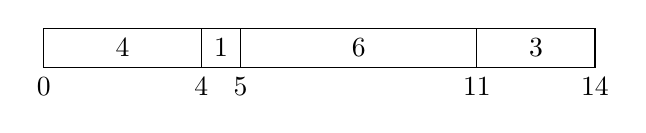
\begin{tikzpicture}[scale = 0.5]
		\draw (0,0)rectangle(4,1)rectangle(5,0)rectangle(11,1)rectangle(14,0);
		\node [anchor=north] at (0,0)  {0};
		\node [anchor=north] at (4,0)  {4};
		\node [anchor=north] at (5,0)  {5};
		\node [anchor=north] at (11, 0)  {11};
		\node [anchor=north] at (14,0)  {14};

		\node at (2,0.5)  {4};
		\node at (4.5,0.5)  {1};
		\node at (8,0.5)  {6};
		\node at (12.5,0.5)  {3};
	\end{tikzpicture}
\end{center}
il tempo di completamento di questa disposizione è
\[
	\frac{4 + 5 + 11 + 14}{4} = \frac{34}{4} = 8.5
\]
\subsubsection{Soluzione}
\begin{itemize}
	\item Ordino le task per lunghezza crescente
\end{itemize}
Prendendo una permutazione ottima in cui a indice $ m $ si trova la task più corta, posso scambiarla con il primo elemento ottenendo che:
\begin{itemize}
	\item Per $ i>m $ le task hanno lo stesso tempo di completamento rispetto a prima dello scambio
	\item Per $ i<m $ le task hanno tempo di completamento $ \le $ rispetto a prima dello scambio
\end{itemize}
Quindi scambiando posso migliorare la soluzione
\subsection{Zaino frazionario}
Abbiamo un array di pesi e pressi rispettivamente $ w\left[i\right] $ e $ p\left[i\right] $ e una capacità $ C $. Trovare la quantità di ciascun oggetto per massimizzare il profitto senza eccedere la capacità. La quantità può essere frazionaria

\subsubsection{Soluzione}
\begin{itemize}
	\item Ordino per \textit{profitto specifico descrescente} (\verb|p[i]/w[i]|)
	\item Prendo quanto più possibile di ogni oggetto, a partire da quello con profitto specifico più alto
\end{itemize}
Informalmente posso dire che se l'oggeto con il peso specifico maggiore occupa $ x $, non ha senso riempire questo spazio in parte con "oro" e il resto con argento, ma conviere riempire tutto con oro
\subsection{Compressione di Huffman}
Idea di base:
\begin{itemize}
	\item Un file può essere rappresentato come stream di caratteri, dove ogni carattere ha una codifica binaria (es \verb|a = 01100001|)
	\item Possiamo associare a sequenze che si ripetono spesso dei codici più corti, così da risparmiare spazio (es \verb|a = 01100001 | $ \rightarrow  $ \verb|001|)
\end{itemize}
Per identificare un carattere si possono usare degli alberi di parsing come segue:
\vskip3mm
\begin{minipage}[c]{0.48\textwidth}
	\begin{center}
		\begin{forest}
			for tree={draw,circle, grow = -90}
			[
			[, edge label={node[midway,left, font=\tiny]{0}}
						[a, edge label={node[midway,left, font=\tiny]{0}}]
						[, edge label={node[midway,right, font=\tiny]{1}}
								[b, edge label={node[midway,left, font=\tiny]{0}}]
								[c, edge label={node[midway,right, font=\tiny]{1}}]
						]
				]
				[, edge label={node[midway,right, font=\tiny]{1}}
						[d, edge label={node[midway,left, font=\tiny]{0}}]
						[e, edge label={node[midway,right, font=\tiny]{1}}]
				]
			]
		\end{forest}
		\vskip3mm
		\begin{tabular}{ccccc}
			\toprule
			a           & b            & c            & d           & e           \\
			\midrule
			\texttt{00} & \texttt{010} & \texttt{011} & \texttt{10} & \texttt{11} \\
			\bottomrule
		\end{tabular}
	\end{center}
\end{minipage}%
\hfill
\begin{minipage}[c]{0.48\textwidth}
	\begin{algoritmo}{Huffmann}
		\begin{algorithm}[H]
			\caption{Algoritmo di decodifica}
			parti dalla radice\;
			\While{file non è finito}{
				leggi un bit\;
				\If{bit è zero}{
					vai a sinistra\;
				}
				\Else{
					vai a destra\;
				}
				\If{nodo foglia}{
					stampa il carattere\;
					torna alla radice\;
				}
			}
		\end{algorithm}
	\end{algoritmo}
\end{minipage}
\vskip3mm
Siccome i caratteri possono essere codificati a lunghezza variabile in base alla frequenza con cui compaiono si possono costruire alberi di parsing più o meno efficienti:
\begin{table}[H]
	\centering
	\begin{tabular}{cccccccc}
		\toprule
		Caratteri  & a                               & b                                & c                                & d                                & e                                & f                                & Dim.    \\
		\midrule
		Frequenza  & 45\%                            & 13\%                             & 12\%                             & 16\%                             & 9\%                              & 5\%                              &         \\
		ASCII      & \footnotesize \texttt{01100001} & \footnotesize  \texttt{01100010} & \footnotesize  \texttt{01100011} & \footnotesize  \texttt{01100100} & \footnotesize  \texttt{01100101} & \footnotesize  \texttt{01100110} & $8n$    \\
		Codifica 1 & \footnotesize \texttt{000}      & \footnotesize \texttt{001}       & \footnotesize\texttt{010}        & \footnotesize \texttt{011}       & \footnotesize\texttt{101}        & \footnotesize \texttt{101}       & $3n$    \\
		Codifica 2 & \footnotesize \texttt{0}        & \footnotesize \texttt{101}       & \footnotesize\texttt{100}        & \footnotesize \texttt{111}       & \footnotesize\texttt{1101}       & \footnotesize \texttt{1100}      & $2.24n$ \\
		\bottomrule
	\end{tabular}
	\caption{Tabella comparativa delle codifiche}
\end{table}
\[
	\text{Costo totale: } (0.45 \cdot 1 + 0.13 \cdot 3 + 0.12 \cdot 3 + 0.16 \cdot 3 + 0.09 \cdot 4 + 0.05 \cdot 4) \cdot n = 2.24n
\]

Note come nel caso della codifica $ 3 $, devo scegliere un insieme di stringhe binarie che non condividono alcun prefisso, altrimenti si rischierebbe di avere un conflitto durante il riconoscimento, ad esempio:
\[
	a = \text{\ttfamily 0} \quad
	b = \text{\ttfamily 1} \quad
	c = \text{\ttfamily 11}
\]
la stringa
\begin{center}
	\ttfamily 0111
\end{center}
ha interpretazione ambigua




\subsubsection{Costruzione albero di parsing ideale}
Per costruire un albero di parsing ottimale si può procedere così:
\begin{itemize}
	\item Creare una lista di nodi foglia, ognuno con carattere e il relativo numero di occorrenze nel file
	\item Rimuovere i due nodi con frequenze minori $f_x, f_y$
	\item Creare un nodo padre con etichetta \texttt{"-"} e frequenza $f_x + f_y$
	\item Collegare i due nodi rimossi con il nuovo nodo
	\item Aggiungere il nodo così creato all’insieme
\end{itemize}

\begin{center}
	\begin{forest}
		for tree={draw, grow = -90, font=\ttfamily}
		[,draw=none
		[f: 5, no edge, name=a]
		[e: 9, no edge, name=b]
		[c: 12, no edge, name=c]
		[b: 13, no edge, name=d]
		[d: 16, no edge, name=e]
		[a: 45, no edge, name=f]
		]
		\node[draw, dashed, mutedred, fit=(a) (b) (c) (d) (e) (f)] {};
	\end{forest}
	\vskip3mm
	\begin{forest}
		for tree={draw, grow = -90, font=\ttfamily}
		[,draw=none
		[c: 12, no edge, name=a]
		[b: 13, no edge, name=b]
		[-: 14, no edge, name=c
		[f: 5]
		[e: 9]
		]
		[d: 14, no edge, name=d]
		]
		\node[draw, dashed,mutedred, fit=(a) (b) (c) (d)] {};
	\end{forest}%
	\vskip3mm
	\begin{forest}
		for tree={draw, grow = -90, font=\ttfamily}
		[,draw=none
		[-: 14, no edge, name=a
		[f: 5]
		[e: 9]
		]
		[d: 16, no edge, name=b]
		[-: 25, no edge, name=c
		[c: 12]
		[b: 13]
		]
		[a: 45, no edge, name=d]
		]
		\node[draw, dashed, mutedred, fit=(a) (b) (c) (d)] {};
	\end{forest}
	\vskip3mm
	\begin{forest}
		for tree={draw, grow = -90, font=\ttfamily}
		[,draw=none
		[-: 25, no edge, name=a
		[c: 12]
		[b: 13]
		]
		[-: 30, no edge, name=b
		[-: 14
			[f: 5]
			[e: 9]
		]
		[d: 16]
		]
		[a: 45, no edge, name=c]
		]
		\node[draw, dashed, mutedred, fit=(a) (b) (c)] {};
	\end{forest}
\end{center}

\vskip3mm

\begin{minipage}[c]{0.48\textwidth}
	\begin{forest}
		for tree={draw, grow = -90, font=\ttfamily}
		[,draw=none
		[a: 45, no edge, name=a]
		[-: 55, no edge, name=b
		[-: 25
			[c: 12]
			[b: 13]
		]
		[-: 30
			[-: 14
					[f: 5]
					[e: 9]
			]
			[d: 16]
		]
		]
		]
		\node[draw, dashed, mutedred, fit=(a) (b)] {};
	\end{forest}
\end{minipage}
%
\begin{minipage}[c]{0.48\textwidth}
	\begin{forest}
		for tree={draw, grow = -90, font=\ttfamily}
		[-: 100, no edge, name=a
		[a: 45]
		[-: 55
			[-: 25
					[c: 12]
					[b: 13]
			]
			[-: 30
					[-: 14
							[f: 5]
							[e: 9]
					]
					[d: 16]
			]
		]
		]
		\node[draw, dashed, mutedred, fit=(a)] {};
	\end{forest}
\end{minipage}
\begin{figure}[H]
	\centering
	\begin{minipage}[c]{0.48\textwidth}
		\begin{forest}
			for tree={draw, grow = -90, font=\ttfamily}
			[-: 100, no edge, name=root
			[a: 45, edge label={node[midway,left, font=\tiny]{0}}]
			[-: 55, edge label={node[midway,right, font=\tiny]{1}}
				[-: 25, edge label={node[midway,left, font=\tiny]{0}}
						[c: 12, edge label={node[midway,left, font=\tiny]{0}}]
						[b: 13, edge label={node[midway,right, font=\tiny]{1}}]
				]
				[-: 30, edge label={node[midway,right, font=\tiny]{1}}
						[-: 14, edge label={node[midway,left, font=\tiny]{0}}
								[f: 5, edge label={node[midway,left, font=\tiny]{0}}]
								[e: 9, edge label={node[midway,right, font=\tiny]{1}}]
						]
						[d: 16, edge label={node[midway,right, font=\tiny]{1}}]
				]
			]
			]
			\node[draw, dashed, mutedred, fit=(root)] {};
		\end{forest}
	\end{minipage}
	%
	\begin{minipage}[c]{0.48\textwidth}
		\begin{center}
			\begin{tabular}{ccccc}
				\toprule
				a           & b            & c            & d           & e           \\
				\midrule
				\texttt{00} & \texttt{010} & \texttt{011} & \texttt{10} & \texttt{11} \\
				\bottomrule
			\end{tabular}
		\end{center}
	\end{minipage}
	\caption{Albero di parsing finale}
\end{figure}
\subsubsection{Dimostrazione}
\begin{itemize}
	\item Consideriamo una soluzione ottima \verb|T|
	\item Consideriamo il carattere \verb|x| con \textit{frequenza più bassa} $ \rightarrow f\left[x\right] $ minima
	\item Consideriamo il carattere \verb|a| con \textit{profondità massima} $ \rightarrow d_T\left[a\right] $ massima
	\item Consideriamo l'albero \verb|T'| ottenuto scambiando \verb|x| con \verb|a|
	\item Dimostriamo che il costo finale di \verb|T'| è $ \le $ di quello di \verb|T|:
	      \begin{align*}
		      C(f, T) - C(f, T') & = \sum_{c \in \Sigma} f[c] d_T(c) - \sum_{c \in \Sigma} f[c] d_{T'}(c)            \\
		                         & = \big(f[x] d_T(x) + f[a] d_T(a)\big) - \big(f[x] d_{T'}(x) + f[a] d_{T'}(a)\big) \\
		                         & = \big(f[x] d_T(x) + f[a] d_T(a)\big) - \big(f[x] d_T(a) + f[a] d_T(x)\big)       \\
		                         & = \big(f[a] - f[x]\big) \big(d_T(a) - d_T(x)\big)                                 \\
		                         & \geq 0
	      \end{align*}
	      quindi
	      \[
		      C(f, T) - C(f, T') \ge 0 \rightarrow  C(f, T') \le C(f, T)
	      \]
\end{itemize}
\subsection{Alberi di copertura minimali}
\begin{definizione}{Albero di copertura}
	Un \underline{albero di copertura} di un grafo $ G = \left(V, E\right) $ è un sottoinsieme di $ E $ che contiene tutti i nodi di $ V $ la cui somma dei pesi è minima
\end{definizione}
\begin{teorema}{Archi sicuri per minimum spanning tree}
	Dato un insieme di archi $ A $ contenuto in qualche albero di copertura e un taglio che rispetti $ A $,
	se $ \left(u,v\right) $ è un arco leggero che attraversa il taglio, allora $ \left(u,v\right) $ è \textit{sicuro per $ A $}
\end{teorema}\label{archi sicuri}
Dimostrazione: considera
\begin{itemize}
	\item $ T $: un albero di copertura minimo.
	\item $ A $: un sottoinsieme degli archi di $ T $
	\item  $ t = \left(S, V-S\right) $ un taglio che rispetti $ A $
	\item $ \left(u, v\right) $ un arco leggero a cavallo di $ t $
	\item $ \left(x,y\right) $ l'arco di $ T $ che attraversa il taglio
\end{itemize}
\begin{minipage}[t]{0.48\textwidth}
	\begin{center}
		\begin{tikzpicture}[node/.style={circle, draw, minimum size=1.5em}]
			\node (u)  [thick, node] {u};
			\node (tl1)[thick, node, below of = u] {};
			\node (tl2)[thick, node, below of = tl1] {};
			\node (tl3)[thick, node, below of = tl2] {};
			\node (x)  [thick, node, below of = tl3] {x};

			\node (v)[node] at (2,0) {v};
			\node (tr1)[node, below of = v] {};
			\node (tr2)[node, below of = tr1] {};
			\node (tr3)[node, below of = tr2] {};
			\node (y)[node, below of = tr3] {y};

			\draw (u)--(v)--(tr1)--(tr2)--(tr3)--(y)--(x)--(tl3)--(tl2)--(tl1)--(u);
			\draw [ultra thick, mutedblue](x)--(tl3)--(tl2)--(tl1)--(u)--(v)--(tr1)-- (tr2)--(tr3)--(y);

			\draw [dashed](1,1)--(1, -5);
		\end{tikzpicture}
		\[
			T
		\]
	\end{center}
\end{minipage}
%
\begin{minipage}[t]{0.48\textwidth}
	\begin{center}
		\begin{tikzpicture}[node/.style={circle, draw, minimum size=1.5em}]
			\node (u)  [thick, node] {u};
			\node (tl1)[thick, node, below of = u] {};
			\node (tl2)[thick, node, below of = tl1] {};
			\node (tl3)[thick, node, below of = tl2] {};
			\node (x)  [thick, node, below of = tl3] {x};

			\node (v)[node] at (2,0) {v};
			\node (tr1)[node, below of = v] {};
			\node (tr2)[node, below of = tr1] {};
			\node (tr3)[node, below of = tr2] {};
			\node (y)[node, below of = tr3] {y};

			\draw (u)--(v)--(tr1)--(tr2)--(tr3)--(y)--(x)--(tl3)--(tl2)--(tl1)--(u);
			\draw [ultra thick, mutedblue](x)--(tl3)--(tl2)--(tl1)--(u)++(v)--(tr1)-- (tr2)--(tr3)--(y);
			\draw [ultra thick, mutedblue](x)--(y);

			\draw [dashed](1,1)--(1, -5);
		\end{tikzpicture}
		\[
			T'
		\]
	\end{center}
\end{minipage}
\vskip3mm
Dove i nodi con contorno grossi costituiscono $ A $ e gli edge blue costituiscono appartengono all'albero di copertura
\begin{itemize}
	\item Se $ \left(u,v\right) \in T $ allora è per forza sicuro
	\item Se $ \left(u,v\right) \not \in T $ allora procedo così:
	      \begin{itemize}
		      \item Considero un taglio che sia trapassato da $ u,v $
		      \item Esisterà un arco $ \left(x,y\right) $ che attraversa il taglio
		      \item Se considero $ T' = T - \left\{x,y\right\} + \left\{u,v\right\} $
		            \begin{itemize}
			            \item $ T' $ è più leggero di $ T $ in quanto $ w\left(u,v\right) \le w \left(x,y\right) $ ($ \left(u,v\right) $ è leggero)
			            \item $ T $ è più leggero di $ T' $ in quanto è \textit{minimum spanning tree}
		            \end{itemize}
	      \end{itemize}
\end{itemize}

\subsubsection{Algoritmo di kruskal}\label{algoritmo di kruskal}
Secondo quanto dimostrato nel \hyperref[archi sicuri]{teorema sugli archi sicuri}, posso costruire un albero di copertura minimo in questo modo:
\begin{itemize}
	\item Ogni nodo appartiene inizialmente a un gruppo diverso
	\item Scorro gli edge in ordine di peso crescente
	\item Se l'edge connette due nodi che appartengono a gruppi diversi allora posso unire il gruppo. Altrimenti non aggiungo nulla, se no introdurrei un ciclo
	\item L'albero viene registrato come \verb|set<edges>|
\end{itemize}

\begin{algoritmo}{Kruskal MSPT}
	\begin{algorithm}[H]
		\caption{Kruskal's Algorithm}

		\SetKwFunction{Find}{find}
		\SetKwFunction{Merge}{merge}
		\SetKwFunction{Insert}{insert}
		\SetKwFunction{Kruskal}{kruskal}
		\SetKwData{Edge}{Edge}
		\SetKwData{MFSet}{MFSet}

		\Fn{$ \Set<\Edge> $ \Kruskal$(\Edge[]\ A,\ \Int\ n,\ \Int\ m)$}{
			\Set $T = \textnormal{Set()}$\;
			\MFSet $M = \textnormal{Mfset}(n)$\;
			\Comment{\textcolor{mutedblue}{ordina gli edge per peso crescente}}
			\textnormal{int} $count = 0$\;
			\textnormal{int} $i = 1$\;
			\Comment{\textcolor{mutedblue}{Termina quando l'albero ha $n - 1$ archi o non ci sono più archi}}
			\While{$count < n - 1$ \textnormal{and} $i \leq m$}{
				\If{$M.\Find(A[i].u) \neq M.\Find(A[i].v)$}{
					$M.\Merge(A[i].u, A[i].v)$\;
					$T.\Insert(A[i])$\;
					$count = count + 1$\;
				}
				$i = i + 1$\;
			}
			\Return $T$\;
		}
	\end{algorithm}
\end{algoritmo}

\begin{center}
	\begin{tabular}{lcc}
		\toprule
		Fase                                              & Volte  & Costo         \\
		\midrule
		Inizializzazione                                  & 1      & $O(n)$        \\
		Ordinamento                                       & 1      & $O(m \log m)$ \\
		Operazioni {\ttfamily find()},{\ttfamily merge()} & $O(m)$ & $O(1)^{(*)}$  \\
		\bottomrule
	\end{tabular}
\end{center}
Quindi la complessità dell'algoritmo di Kruskal è:
\[
	O\left(m \log m\right)
\]

% \begin{center}
% 	\begin{tabular}{c}
% 		\toprule
% 		Complessità                             \\
% 		\midrule
% 		$ O\left(m \log \left(m\right)\right) $ \\
% 		\bottomrule
% 	\end{tabular}
% \end{center}
Nota che $ O\left(m \log \left(m\right)\right)  = O\left(m \log \left(n^2 \right)\right) = O\left(m \log \left(n\right)\right)$
\subsubsection{Algoritmo di Prim}
A differenza dell' \hyperref[algoritmo di kruskal]{algoritmo di Kruskal}, l'algoritmo di Prim usa una \textit{priority queue} e ritorna l'albero di copertura come \emph{vettore dei padri}
\begin{itemize}
	\item Mantengo un unico albero $ T $
	\item Creo taglio fra vertici contenuti dell'albero e altri vertici: $ t = \left(T, V-A\right) $
	\item Aggiungo ad ogni iterazione un arco leggero di $ t $
\end{itemize}
\vskip3mm
\begin{algoritmo}{Prim MSPT}
	\begin{algorithm}[H]
		\caption{Prim's Algorithm}

		\SetKwFunction{Insert}{insert}
		\SetKwFunction{DeleteMin}{deleteMin}
		\SetKwFunction{Decrease}{decrease}
		\SetKwFunction{IsEmpty}{isEmpty}
		\SetKwData{PriorityQueue}{PriorityQueue}
		\SetKwData{PriorityItem}{PriorityItem}
		\SetKwData{Node}{Node}
		\SetKwData{Graph}{Graph}

		\Fn{\Int[] prim$(\Graph\ G,\ \Node\ r)$}{
			\PriorityQueue $Q = \textnormal{MinPriorityQueue()}$\;
			\PriorityItem[] $pos = \textnormal{new PriorityItem}[1 \ldots G.n]$\;
			\textnormal{int[]} $p = \textnormal{new int}[1 \ldots G.n]$\;

			\ForEach{$u \in G.V() \setminus \{r\}$}{
				$pos[u] = Q.\Insert(u, +\infty)$\;
			}
			$pos[r] = Q.\Insert(r, 0)$\;
			$p[r] = 0$\;

			\While{\textnormal{not} $Q.\IsEmpty()$}{
				\Node $u = Q.\DeleteMin()$\;
				$pos[u] = \textnormal{nil}$\;

				\ForEach{$v \in G.\textnormal{adj}(u)$}{
					\If{$pos[v] \neq \textnormal{nil}$ \textnormal{and} $w(u, v) < pos[v].\textnormal{priority}$}{
						$Q.\Decrease(pos[v], w(u, v))$\;
						$p[v] = u$\;
					}
				}
			}
			\Return $p$\;
		}
	\end{algorithm}
\end{algoritmo}

\begin{center}
	\begin{tabular}{lcc}
		\toprule
		Fase                           & Volte  & Costo         \\
		\midrule
		Inizializzazione               & 1      & $O(n \log n)$ \\
		{\ttfamily deleteMin()}        & $O(n)$ & $O(\log n)$   \\
		{\ttfamily decreasePriority()} & $O(m)$ & $O(\log n)$   \\
		\bottomrule
	\end{tabular}
\end{center}

Quindi la complessità dell'algoritmo di Prim è:
\[
	O\left(m \log n\right)
\]


\section{Rete di flussi - Fork-Folkerson}
Ho un grafo che rappresenta una rete di \textit{"manichette"} d'acqua, ossia un grafo orientato tale che:
\begin{itemize}
	\item Nodo sorgente $ s \in  V $
	\item Nodo pozzo $ t \in V $
	\item Funzione di capacità: $ c : V \times  V \rightarrow \R \ge 0 $ tale che $ \left(x,y\right) \not \in  E \Rightarrow c\left(x, y\right) = 0 $. Di fatto il peso degli archi indica quanta acqua può passare
\end{itemize}
\subsubsection{Flusso}
Il flusso è una funzione che indica lo scorrimento di acqua in ogni manichetta e gode di 3 proprietà:
\begin{itemize}
	\item Vincolo sulla capacità: non può passare può acqua della portata di una manichetta
	\item Antisimmetria: $ f\left(x,y\right) = -f\left(y,x\right) $. Di fatto aggiungo un arco al contrario da quale posso far passare l'acqua per \textit{"correggere gli errori"}, ossia evito di mandare acqua per un percorso in favore di un altro
	\item Conservazioe del flusso: il flusso totale entrante su di ogni nodo è uguale al flusso uscente, ad eccezione di $ s  $ e $ t $\label{conservazione del flusso}

\end{itemize}
L'algoritmo consiste in :
\begin{itemize}
	\item Trovo percorso da $ s $ a $ t $ e delle manichette che passo prendo il prezzo minore
	\item Sottraggo questo peso a tutti gli archi del percorso e lo aggiungo agli archi inversi (i quali sono inizialmente \underline{inizializzati a zero})
	\item Ripeto algoritmo finchè non è più possibile trovare percorso sa $ s  $ a  $ t $
\end{itemize}

\vskip3mm
\begin{minipage}[t]{0.48\textwidth}
	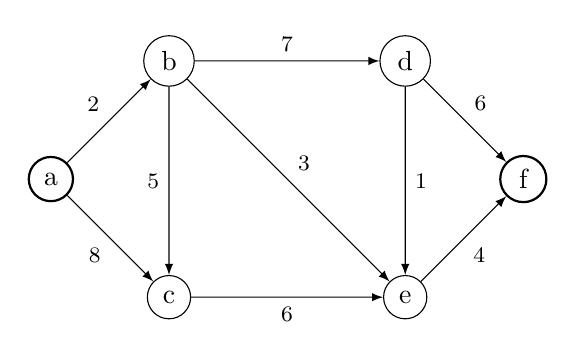
\begin{tikzpicture}[node/.style={circle, draw, minimum size=1.5em}, scale = 1.5, edge/.style={font=\footnotesize, -latex}, bent edge/.style={font=\footnotesize, -latex, bend left=15}]
		\node (a)[node, thick] at (0,0){a};

		\node (b)[node] at (1,1){b};
		\node (d)[node] at (3,1){d};

		\node (c)[node] at (1,-1){c};
		\node (e)[node] at (3,-1){e};

		\node (f)[node, thick] at (4,0){f};

		\draw [edge](a)
		edge node[midway, above left]{2}(b)
		edge node[midway, below left]{8}(c);
		\draw [edge](b)
		edge node[midway, above]{7}(d)
		edge node[midway,above right]{3}(e)
		edge node[midway, left]{5}(c);
		\draw [edge](c)
		edge node [midway, below]{6}(e);
		\draw [edge](e)
		edge node [midway, below right]{4}(f);
		\draw [edge](d)
		edge node [midway, above right]{6}(f)
		edge node [midway, right]{1}(e);
	\end{tikzpicture}
\end{minipage}
%
\begin{minipage}[t]{0.48\textwidth}
	\begin{tikzpicture}[node/.style={circle, draw, minimum size=1.5em}, scale = 1.5, edge/.style={font=\footnotesize, -latex}, bent edge/.style={font=\footnotesize, -latex, bend left=15}]
		\node (a)[node, thick] at (0,0){a};

		\node (b)[node] at (1,1){b};
		\node (d)[node] at (3,1){d};

		\node (c)[node] at (1,-1){c};
		\node (e)[node] at (3,-1){e};

		\node (f)[node, thick] at (4,0){f};

		\draw [edge](a) edge node[midway, below left]{8}(c);
		\draw [edge, edge, mutedred, thick](a) edge node[midway, above left]{2}(b);

		\draw [edge](b) edge node[midway, above]{7}(d) edge node[midway, left]{5}(c);
		\draw [edge, mutedred, thick](b) edge node[midway,above right]{3}(e);

		\draw [edge](c) edge node [midway, below]{6}(e);

		\draw [edge, mutedred, thick](e) edge node [midway, below right]{4}(f);

		\draw [edge](d) edge node [midway, above right]{6}(f) edge node [midway, right]{1}(e);
	\end{tikzpicture}
\end{minipage}
\vskip3mm
\begin{minipage}[t]{0.48\textwidth}
	\begin{tikzpicture}[node/.style={circle, draw, minimum size=1.5em}, scale = 1.5, edge/.style={font=\footnotesize, -latex}, bent edge/.style={font=\footnotesize, -latex, bend left=15}]
		\node (a)[node, thick] at (0,0){a};

		\node (b)[node] at (1,1){b};
		\node (d)[node] at (3,1){d};

		\node (c)[node] at (1,-1){c};
		\node (e)[node] at (3,-1){e};

		\node (f)[node, thick] at (4,0){f};

		\draw [bent edge, mutedred, thick](a) edge node[midway, above left]{2}(b);
		\draw [bent edge, dashed, mutedblue](b) edge node[midway, below right]{-2}(a);

		\draw [edge](a) edge node[midway, below left]{8}(c);

		\draw [edge](b)
		edge node[midway, above]{7}(d)
		edge node[midway, right]{5}(c);

		\draw [bent edge, mutedred, thick](b) edge node[midway,above right]{3}(e);
		\draw [bent edge, dashed, mutedblue](e) edge node[midway,below left]{-3}(b);

		\draw [edge](c)
		edge node [midway, below]{6}(e);

		\draw [bent edge, mutedred, thick](e) edge node [midway, above left]{2}(f);
		\draw [bent edge, dashed, mutedblue](f) edge node [midway, below right]{-2}(e);

		\draw [edge](d)
		edge node [midway, above right]{6}(f)
		edge node [midway, left]{1}(e);

	\end{tikzpicture}
\end{minipage}
%
\begin{minipage}[t]{0.48\textwidth}
	\begin{tikzpicture}[node/.style={circle, draw, minimum size=1.5em}, scale = 1.5, edge/.style={font=\footnotesize, -latex}, bent edge/.style={font=\footnotesize, -latex, bend left=15}]
		\node (a)[node, thick] at (0,0){a};

		\node (b)[node] at (1,1){b};
		\node (d)[node] at (3,1){d};

		\node (c)[node] at (1,-1){c};
		\node (e)[node] at (3,-1){e};

		\node (f)[node, thick] at (4,0){f};

		\draw [bent edge, mutedred, thick](a) edge node[midway, above left]{2}(b);
		\draw [bent edge, dashed, mutedblue](b) edge node[midway, below right]{-2}(a);

		\draw [bent edge, mutedgreen, thick](a) edge node[midway, above right]{8}(c);
		\draw [bent edge, mutedblue, dashed](c) edge node[midway, below left]{-8}(a);

		\draw [edge](b)
		edge node[midway, above]{7}(d)
		edge node[midway, right]{5}(c);

		\draw [bent edge, mutedred, thick](b) edge node[midway,above right]{3}(e);
		\draw [bent edge, dashed, mutedblue](e) edge node[midway,below left]{-3}(b);

		\draw [bent edge, mutedgreen, thick](c) edge node [midway, above]{6}(e);
		\draw [bent edge, mutedblue, dashed](e) edge node [midway, below]{6}(c);

		\draw [bent edge, mutedred, thick](e) edge node [midway, above left]{2}(f);
		\draw [edge, mutedgreen, thick](e) edge (f);
		\draw [bent edge, dashed, mutedblue](f) edge node [midway, below right]{-2}(e);

		\draw [edge](d)
		edge node [midway, above right]{6}(f)
		edge node [midway, left]{1}(e);

	\end{tikzpicture}
\end{minipage}
\vskip3mm
% \begin{center}
% 	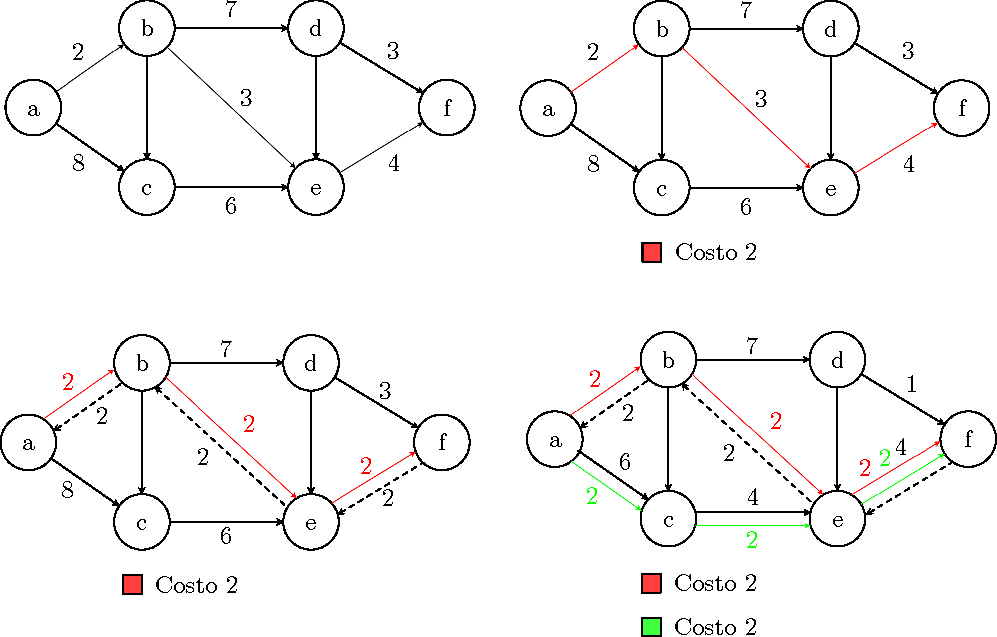
\includegraphics{Images/Rete di flusso.pdf }
% \end{center}
Nota come, quando passo su di un arco inverso è come dire
\begin{center}
	\textit{Ok, evita di mandarmi questa data quantità di acqua, tanto io manderò la stessa quantità al nodo alla quale tu la mandavi. Allo stesso modo, ti trovero un percorso che arrivi a $ t $ cosisshè tu possa far confluire la quantità di acqua che hai evitato di mandarmi}
\end{center}

\subsubsection{Complessità}
\begin{center}
	\begin{tabular}{cc}
		\toprule
		Algoritmo      & Complessità                         \\
		\midrule
		Ford-Fulkerson & $ O\left(E \left|f*\right|\right) $ \\
		Edmonds-Karp   & $ O\left(V E^2 \right) $            \\
		\bottomrule
	\end{tabular}
\end{center}
Nota che la complessità compare solo $ E $ per il costo delle BFS/DFS siccome nel problema delle reti di flusso il grafo è per forza di cose connesso e dunque $ V = O \left(V\right) $

\begin{definizione}{Flusso per un taglio}
	Dato un taglio $ T = \left(S, T\right) $, il \textit{flusso netto} per esso è definito come
	\[
		\sum_{x \in S,  y \in T}f\left(x,y\right)
	\]

\end{definizione}
\subsubsection{Teorema flusso per un taglio}
\begin{teorema}{Flusso per un taglio}
	Dato un \textit{qualsiasi} taglio $ T \left(S, T\right) $ di una rete di flusso e una funzione di flusso $ f $, allora il flusso per il taglio è uguale al flusso complessivo:
	\[
		\sum_{x \in S,  y \in T} f\left(x,y\right) = \left|f\right|
	\]
\end{teorema}\label{flusso per taglio}
Dimostrazione informale:
\begin{itemize}
	\item Il flusso per un taglio è dato dal peso degli archi del flusso "a cavallo" del taglio stesso
	      \[
		      \sum_{x \in S, y \in T}f \left(x,y\right)
	      \]
	\item Per l'antisimmetria, il flusso per il taglio è dato dalla somma di ogni arco che parte da un vertice $ \in S $ e arriva in un qualsiasi altro $ \in V $, in quanto gli archi fra due vertici $ \in S $ si controbilanciano (\textit{antisimmetria})
	      \[
		      \sum_{x \in S, y \in V}f \left(x,y\right)
	      \]
	\item Posso ora spezzare questa quantità nella somma degli archi che parono dalla sorgente $ s $ e quelli che partono da $ S - \left\{s\right\} $.
	      \[
		      \underbracket[0.1ex]{\sum_{x \in s - \left\{s\right\}, y \in V} f\left(x,y\right)}_{\text{archi che partono da $ S - \left\{s\right\} $}} + \underbracket[0.1ex]{\sum_{y \in V} f\left(s,y\right)}_{\text{archi che partono da $ s $}}
	      \]
	\item Ora ho che per la \hyperref[conservazione del flusso]{conservazione del flusso}, la somma degli archi uscenti da ciascun nodo (salvo $ \left\{s, t\right\} $) è \underline{pari a zero}. Dunque
	      \[
		      \sum_{x \in s - \left\{s\right\}, y \in V} f\left(x,y\right) = 0
	      \]
	      e so anche che per definizione:
	      \[
		      \sum_{y \in V} f\left(s,y\right) = \left|f\right|
	      \]
\end{itemize}
\subsubsection{Teorema capacità taglio minimo}
\begin{teorema}{Capacità del taglio}
	Il flusso massimo è limitato superiormente dalla capacità del taglio minimo, ovvero il taglio la cui capacità è minore fra tutti i tagli.
\end{teorema}
Dimostrazione:
\begin{itemize}
	\item Per il teorema riguardo il \hyperref[flusso per taglio]{flusso per un taglio}, sappiamo che il flusso complessivo è pari al flusso che attraversa un qualsiasi taglio
	\item E' facile capire inoltre che il flusso per un taglio è limitato superiormente dalla capacità di quel taglio, in quando per ogni arco che attraversa il taglio ho che
	      \[
		      f\left(x,y\right) \le c\left(x,y\right)
	      \]
	\item Prendo il taglio con capacità minore $ \rightarrow  $ il flusso non può essere maggiore di questa capacità
\end{itemize}
\subsection{Dimostrazione correttezza}
\begin{teorema}{Flusso massimo, cammini aumentanti e taglio}
	Le seguenti affermazioni sono equivalenti:
	\begin{itemize}
		\item $ f $ è il flusso \textit{massimo}
		\item Non esistono cammini aumentanti
		\item $ \left|f\right| $ è uguale alla capacità del \textit{taglio minimo}
	\end{itemize}
\end{teorema}
L'equivalenza si dimostra circolarmente:
\[
	1 \Rightarrow 2,  \quad 2 \Rightarrow 3, \quad 3 \Rightarrow 1
\]
\begin{enumerate}
	\item $ 1 \Rightarrow 2 $
	      \begin{itemize}
		      \item Se esistessero cammini aumentanti allora sarebbe assurdo che il flusso fosse massimo
	      \end{itemize}
	\item $ 2 \Rightarrow 3 $
	      \begin{itemize}
		      \item Prendo insieme di nodi raggiungibili da $ s $ e lo chiamo $ S $. Considero taglio $ T = \left(S, V-S\right) $
		      \item Tutti gli edge a cavallo del taglio devono essere saturati, altrimenti significa che potrei raggiungere altri nodi da $ s $
		      \item Se un taglio è saturato, questo deve per forza essere il taglio minimo, altrimenti esisterebbe un taglio più piccolo che violerebbe il vincolo sulla capacità
	      \end{itemize}
	\item $ 3 \rightarrow 1 $
	      \begin{itemize}
		      \item Il flusso è limitato superiormente dalla capacità di un qualsiasi taglio
		      \item Se $ \left|F\right| $ è uguale al taglio minimo allora $ f $ è per forza massimo
	      \end{itemize}
\end{enumerate}


\subsection{Dimostrazione complessità Edmonds-Karp}
\subsubsection{Teorema monotonia}
\begin{teorema}{Monotonia distanze in iterazioni edmonds-karp}
	Le distanze minime di un nodo $ v $ dalla sorgente $ s $ ($ d\left(v\right) $) possono solo aumentare dopo ogni volta che aggiorniamo il flusso tramite un cammino aumentante
\end{teorema}\label{monotonia}
Dimostrazione:
\begin{itemize}
	\item Chiamo $ G $ il grafo prima di essere aggiornato e $ G' $ il grafo dopo l'aggiornamento
	\item Suppongo per assurdo che esistano dei nodi con distanza minima minore in $ G' $ rispetto che $ G $
	\item Chiamo $ v $ il nodo con distanza minore fra questi. Considero il seguente shortest path:
	      \vskip3mm
	      \begin{center}
		      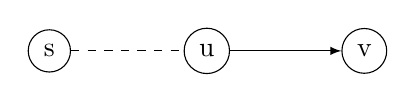
\begin{tikzpicture}
			      \node (a)[draw, circle]at (0,0)  {s};
			      \node (b)[draw, circle]at (2,0)  {u};
			      \node (c)[draw, circle]at (4,0)  {v};
			      \draw (a)[dashed]--(b);
			      \draw (b)[-latex]--(c);
		      \end{tikzpicture}
	      \end{center}
	\item Considero che, siccome $ v $ è il nodo che ha diminuito la distanza \textit{di distanza minima}, allora $ u $ non può aver diminuito la sua distanza:
	      \[
		      d_{\text{dopo}} \left(u\right) \geq d_{\text{prima}} \left(u\right)
	      \]
	\item Dimostro che l'arco $ \left(u,v\right) $ \textit{non} può appartenere a $ G $ in quanto
	      \begin{align*}
		      d_{\text{prima}}\left(v\right) & \le d_{\text{prima}}\left(u\right) + 1 \\
		                                     & \le d_{\text{dopo}} \left(u\right) + 1 \\
		                                     & = d_{\text{dopo}} \left(v\right)
	      \end{align*}
	      quindi $  d_{\text{prima}}\left(v\right) \le d_{\text{dopo}} $, il che contradddice l' ipotesi
	\item Dunque $ \left(u,v\right) \not \in G $ e $ \left(u,v\right) \in G' $. L'unico modo perché questo accada è che l'arco $ \left(u,v\right) $ sia stato "riattivato" percorrendolo al contrario (\textit{con uno shortest path}). Considero dunque
	      \begin{align*}
		      d_{\text{prima}} \left(v\right) & = d_{\text{prima}} \left(u\right) - 1                 \\
		                                      & \le d_{\text{dopo}} \left(u\right) - 1                \\
		                                      & = \left(d_{\text{dopo}} \left(v\right) - 1\right) - 1 \\
	      \end{align*}
	      quindi ancora una volta ottengo che $  d_{\text{prima}}\left(v\right) \le d_{\text{dopo}} - 2 $, il che contradddice l' ipotesi
\end{itemize}

\subsubsection{Dimostrazione complessità edmon karps}
Edmonds-Karp usa BFS. Così facendo si può dimostrare che aumento il flusso massimo $ VE $ volte:
\begin{itemize}
	\item Considero arco $ \left(x,y\right) $. Ogni volta che rimuovo cammino aumentante degli archi si "spengono"
	\item Dimostro che un arco critico $ \left(x,y\right) $ (che fa da collo di bottiglia) aumenta la sua distanza in archi di almeno 2 prima di ritornare critico
	      \begin{itemize}
		      \item Prima di rimuovere cammino aumentante distanza da $ y $ = distanza da $ x + 1 $
		      \item Dopo averlo rimosso, per "riaccendere" arco devo ripercorrerlo al contrario
		      \item Prendendo percorso in cui ripercorro arco al contrario
		      \item Quindi $ d_{\text{ dopo spegnimento }}\left(x\right) =  d_{\text{ dopo spegnimento }}\left(y\right) + 1 $
		      \item Visto che le distanze NON possono diminure ho che
		            \begin{align*}
			            d_{\text{ dopo spegnimento }}\left(x\right) & =  d_{\text{ dopo spegnimento }}\left(y\right) + 1                              \\
			                                                        & \ge d_{\text{ \underline{prima} spegnimento }}\left(y\right) + 1                \\
			                                                        & = \left(d_{\text{ \underline{prima} spegnimento }}\left(x\right) + 1\right) + 1
		            \end{align*}
		      \item Ho dimostrato quindi che la distanza in archi aumenta \underline{almeno di 2} ogni volta che un archo diventa critico
		      \item Dato $ \left(x,y\right) $ con $ d\left(x\right) \le d\left(y\right) $ allora $ d\left(x\right) $ è al massimo $ V - 2 $
		      \item La distanza MINIMA di un nodo non può aumentare all'infinito, quindi, dato che aumenta di $ 2 $ ogni volta, ogni arco può diventare critivo al più $ \frac{\left(V-2\right)}{2} $ volte, ossia $ O\left(V\right) $
		      \item Siccome ci sono $ O\left(E\right) $ archi, al più posso aumentare $ O\left(VE\right) $ volte
	      \end{itemize}
\end{itemize}
\section{Backtracking}
Solitamente i problemi che richiedono una soluzione \textit{brute-force} sono in qualche modo riconducibili a problemi di \textit{combinatoria}. In particolare molti problemi di backtracking sono risolvibili con versioni modificate dei due seguenti algoritmi
\vskip3mm
\subsection{Generete all subsets}
\begin{algoritmo}{Generate all subsets}
	\begin{algorithm}[H]
		\caption{Print Subsets of a Set (Recursive)}
		\SetKwFunction{PrintSubsetsRec}{print\_subsets\_rec}
		\SetKwFunction{PrintSet}{print\_set}
		\Fn{\Void \PrintSubsetsRec$( \Item\ set,\ \Item\ item,\ \Int\ index)$}{
			\If{\textnormal{index} == 0}{
				\PrintSet(\textnormal{set}, \textnormal{choiches})\;
				\Return\;
			}
			\textnormal{choiches[index]} $\gets$ \textnormal{false}\;
			\PrintSubsetsRec(\textnormal{set}, \textnormal{choiches}, \textnormal{index} - 1)\;
			\textnormal{choiches[index]} $\gets$ \textnormal{true}\;
			\PrintSubsetsRec(\textnormal{set}, \textnormal{choiches}, \textnormal{index} - 1)\;
		}


		\SetKwFunction{PrintSubsets}{print\_subsets}
		\SetKwFunction{PrintSubsetsRec}{print\_subsets\_rec}
		\Fn{\Void \PrintSubsets$(\Item\ set)$}{
			\textnormal{choices} $\gets$ \textnormal{empty array}\;
			\For{$i \gets 1$ \KwTo $\textnormal{\#set}$}{
				\textnormal{choices[i]} $\gets$ \textnormal{false}\;
			}
			\PrintSubsetsRec(\textnormal{set}, \textnormal{choices}, \textnormal{\#set})\;
		}
	\end{algorithm}\label{sottoinsiemi}
\end{algoritmo}

\subsection{Generete all permutations}
\begin{algoritmo}{Generate all permutations}
	\begin{algorithm}[H]
		\caption{Print Permutations of a Set (Recursive)}
		\SetKwFunction{PrintPermRec}{print\_perm\_rec}
		\SetKwFunction{PrintArray}{print\_array}
		\Fn{\Void \PrintPermRec$(\Item\ v,\ \Item\ choices,\ \Int\ index)$}{
			\If{\textnormal{index} == 0}{
				\PrintArray(\textnormal{choices})\;
				\Return\;
			}
			\For{$i \gets 1$ \KwTo $\textnormal{\#v}$}{
				\textnormal{choices[index]} $\gets$ \textnormal{v[i]}\;
				\PrintPermRec(\textnormal{v}, \textnormal{choices}, \textnormal{index} - 1)\;
			}
		}

		\caption{Print All Permutations of a Set}
		\SetKwFunction{PrintPerm}{print\_perm}
		\SetKwFunction{PrintPermRec}{print\_perm\_rec}
		\Fn{\Void \PrintPerm$(\Item\ v)$}{
			\textnormal{choices} $\gets$ \textnormal{empty array}\;
			\For{$i \gets 1$ \KwTo $\textnormal{\#v}$}{
				\textnormal{choices[i]} $\gets$ \textnormal{false}\;
			}
			\PrintPermRec(\textnormal{v}, \textnormal{choices}, \textnormal{\#v})\;
		}
	\end{algorithm}
\end{algoritmo}

\subsection{K-sottoinsiemi}
Per questo algoritmo possiamo usare la versione naive, meno efficiente, modificando l'algoritmo \hyperref[sottoinsiemi]{dei sottoinsiemi}
\vskip3mm
\begin{algoritmo}{K-subsets naif}
	\begin{algorithm}[H]
		\caption{Print Subsets of a Set (Recursive)}
		\SetKwFunction{PrintSubsetsRec}{print\_subsets\_rec}
		\SetKwFunction{CountOnes}{count\_ones}
		\SetKwFunction{PrintSet}{print\_set}
		\Fn{\Void \PrintSubsetsRec$( \Item\ set,\ \Item\ item,\ \Int\ index,\ \Int\ k)$}{
			\If{\textnormal{index} == 0 \textcolor{mutedred}{\And \CountOnes{choices} == k}}{
				\PrintSet(\textnormal{set}, \textnormal{choiches})\;
				\Return\;
			}
			\textnormal{choiches[index]} $\gets$ \textnormal{false}\;
			\PrintSubsetsRec(\textnormal{set}, \textnormal{choiches}, \textnormal{index} - 1)\;
			\textnormal{choiches[index]} $\gets$ \textnormal{true}\;
			\PrintSubsetsRec(\textnormal{set}, \textnormal{choiches}, \textnormal{index} - 1)\;
		}

	\end{algorithm}
\end{algoritmo}
\vskip3mm

Possiamo utilizzare una verisone molto più ottimizzata utilizzando un pruning:
\vskip3mm
\begin{algoritmo}{K-subsets con pruning}
	\begin{algorithm}[H]
		\caption{kssRec (Recursive Subset Sum Algorithm)}
		\SetKwFunction{KSSRec}{kssRec}
		\SetKwFunction{ProcessSolution}{processSolution}
		\Fn{\Void \KSSRec$(\Int\ n,\ \Int\ missing,\ \Int[]\ S,\ \Int\ i)$}{
			\If{$\textnormal{missing} == 0$}{
				\ProcessSolution$(S, i - 1)$\;
				\Return\;
			}
			\ElseIf{$i \leq n$ \textnormal{and} $0 < \textnormal{missing} \leq n - (i - 1)$}{
				\ForEach{$c \in \{0, 1\}$}{
					$S[i] \gets c$\;
					\KSSRec$(n, \textnormal{missing} - c, S, i + 1)$\;
				}
			}
		}
	\end{algorithm}
\end{algoritmo}

\begin{center}
	\begin{forest}
		for tree={draw, grow = -90, draw, circle}
		[
		[, edge label={node[midway,left, font=\tiny]{0}}
					[, edge label={node[midway,left, font=\tiny]{0}}
							[,fill=mutedblue!50, edge label={node[midway,left, font=\tiny]{0}}
									[, edge label={node[midway,left, font=\tiny]{0}}]
									[, edge label={node[midway,right, font=\tiny]{1}}]
							]
							[, edge label={node[midway,right, font=\tiny]{1}}
									[, edge label={node[midway,left, font=\tiny]{0}}]
									[,fill=mutedred!50, edge label={node[midway,right, font=\tiny]{1}}]
							]
					]
					[, edge label={node[midway,right, font=\tiny]{1}}
							[, edge label={node[midway,left, font=\tiny]{0}}
									[,  edge label={node[midway,left, font=\tiny]{0}}]
									[,fill=mutedred!50, edge label={node[midway,right, font=\tiny]{1}}]
							]
							[,fill=mutedred!50, edge label={node[midway,right, font=\tiny]{1}}
									[, dashed, edge={dashed}, edge label={node[midway,left, font=\tiny]{0}}]
									[, dashed, edge={dashed}, edge label={node[midway,right, font=\tiny]{1}}]
							]
					]
			]
			[, edge label={node[midway,right, font=\tiny]{1}}
					[, edge label={node[midway,left, font=\tiny]{0}}
							[, edge label={node[midway,left, font=\tiny]{0}}
									[, edge label={node[midway,left, font=\tiny]{0}}]
									[,fill=mutedred!50, edge label={node[midway,right, font=\tiny]{1}}]
							]
							[,fill=mutedred!50, edge label={node[midway,right, font=\tiny]{1}}
									[, dashed, edge={dashed}, edge label={node[midway,left, font=\tiny]{0}}]
									[, dashed, edge={dashed}, edge label={node[midway,right, font=\tiny]{1}}]
							]
					]
					[,fill=mutedred!50, edge label={node[midway,right, font=\tiny]{1}}
							[, dashed, edge={dashed}, edge label={node[midway,left, font=\tiny]{0}}
									[, dashed, edge={dashed}, edge label={node[midway,left, font=\tiny]{0}}]
									[, dashed, edge={dashed}, edge label={node[midway,right, font=\tiny]{1}}]
							]
							[, dashed, edge={dashed}, edge label={node[midway,right, font=\tiny]{1}}
									[, dashed, edge={dashed}, edge label={node[midway,left, font=\tiny]{0}}]
									[, dashed, edge={dashed}, edge label={node[midway,right, font=\tiny]{1}}]
							]
					]
			]
		]
	\end{forest}
\end{center}
\vskip3mm
Utilizzando il \textit{pruning}, andiamo a risparmiare un sacco di salcolo (guarda i nodi tratteggiati). In particolare

\subsection{Subset sum}\label{subset sum}
Dato un insieme di interi positivi \verb|A| e un numero intero positivo \verb|k|, ritornare \verb|true| se esiste una combinazione di elementi di \verb|A| che sommati danno \verb|k|
\vskip3mm
\begin{algoritmo}{Subset sum}
	\begin{algorithm}[H]
		\caption{Recursive Subset Sum with Solution Printing}
		\SetKwFunction{SSRec}{ssRec}
		\SetKwFunction{ProcessSolution}{processSolution}

		\Fn{\Bool \SSRec$(\Int[]\ A,\ \Int\ n,\ \Int\ missing,\ \Int[]\ S,\ \Int\ i)$}{
			\If{$\textnormal{missing} == 0$}{
				\ProcessSolution$(S, i - 1)$ \Comment*[r]{\textcolor{mutedblue}{Stampa gli indici della soluzione}}
				\Return \KwTrue\;
			}
			\ElseIf{$i > n$ \Or $\textnormal{missing} < 0$}{
				\Comment{\textcolor{mutedblue}{Terminati i valori o somma eccessiva}}
				\Return \KwFalse\;
			}
			\Else{
				\ForEach{$c \in \{0, 1\}$}{
					$S[i] \gets c$\;
					\If{\SSRec$(A, n, \textnormal{missing} - A[i] \cdot c, S, i + 1)$}{
						\Return \KwTrue\;
					}
				}
				\Return \KwFalse\;
			}
		}
	\end{algorithm}
\end{algoritmo}
\vskip3mm
\verb|missing| tiene conto della somma mancante da riempire per arrivare a \verb|k|.
\subsection{Problema delle 8 regine}
Supponiamo di avere \verb|n| regine da disporre in una griglia quadrata \verb|nxn|. Una regina "minaccia" un'altra regine sa sono sulla stessa riga, colonna o diagonale. Il problema consiste nel disporre le regine in modo tale che nessuna di esse possa "prendere" un'altra. Vediamo un'ottimizzazione alla volta
\begin{itemize}
	\item Numeriamo posizioni scacchiera da $ 1 $ a $ 64 $. Ogni posizione può avere una regina oppure no.
	      \[
		      \text{Complessità: } 2^{n^2} = 2^{64} = \approx 1.84 \cdot 10^{19}
	      \]
	\item Visto che dobbiamo piazzare solo $ 8 $ regine, possiamo considerare un vettore \verb|v[1...8]| con \verb|v[i] = posizione i-esima regina|. Ogni cella ha $ 64 $ possibilità, quindi:
	      \[
		      \text{Complessità: } \left(n^2 \right)^{n} = 64^{8} = \approx 2.81 \cdot 10^{14}
	      \]
	\item Evito di considerare permutazioni di schieramenti. Quando piazzo la regina $ i $, considero solo le posizioni $ > $ rispetto alla posizione della regina $ i-1 $. Dato che per ogni schieramento non calcolo le permutazioni il costo è di
	      \[
		      \text{Complessità: } \frac{\left(n^2 \right)^{n}}{n!} = \frac{64^{8}}{8!} \approx 6.98 \cdot 10^{9}
	      \]
	\item Considero che ogni colonna della scacchiera contiene esattamente $ 1 $ regina, altrimenti ci sarebbero regine che si minacciano. Ognuna delle $ n $ colonne ha $ n $ possibili posizioni:
	      \[
		      \text{Complessità: } \left(n \right)^{n} =8^8 \approx 1.67 \cdot  10^7
	      \]
	\item Se piazzo una regina in una riga $ j $, allora non potrò piazzare nessuna delle regine successive in quella colonna. Quindi ogni colonna le posizioni possibili diminuiscono:

	      \[
		      \text{Complessità: } n! = 8! = 40320
	      \]

\end{itemize}
\subsection{Sudoku}
\begin{algoritmo}{Sudoku}
	\begin{algorithm}[H]
		\caption{Sudoku Solver}
		\SetKwFunction{Sudoku}{sudoku}
		\SetKwFunction{Moves}{moves}
		\SetKwFunction{ProcessSolution}{processSolution}

		\Fn{\Bool \Sudoku$(\Int[][]\ S,\ \Int\ i)$}{
			\If{$i == 81$}{
				\ProcessSolution$(S, n)$ \Comment*[r]{Process the completed solution}
				\Return \KwTrue\;
			}
			\textnormal{int} $x = i \mod 9$\;
			\textnormal{int} $y = \lfloor i / 9 \rfloor$\;
			\Set $C = \Moves(S, x, y)$\;
			\textnormal{int} $old = S[x][y]$\;
			\ForEach{$c \in C$}{
				$S[x][y] = c$\;
				\If{\Sudoku$(S, i + 1)$}{
					\Return \KwTrue\;
				}
			}
			$S[x][y] = old$\;
			\Return \KwFalse\;
		}

		\vskip3mm
		\SetKwFunction{Moves}{moves}
		\SetKwFunction{Check}{check}
		\Fn{\Set \Moves$(\Int[][]\ S,\ \Int\ x,\ \Int\ y)$}{
			\Set $C = \textnormal{Set()}$\;
			\If{$S[x][y] \neq 0$}{
				$C.\textnormal{insert}(S[x][y])$ \Comment*[r]{Pre-inserted number}
			}
			\Else{
				\Comment{Check for conflicts}
				\For{$c = 1$ \KwTo $9$}{
					\If{\Check$(S, x, y, c)$}{
						$C.\textnormal{insert}(c)$\;
					}
				}
			}
			\Return $C$\;
		}

		\Fn{\Bool \Check$(\Int[][]\ S,\ \Int\ x,\ \Int\ y,\ \Int\ c)$}{
			\Comment{Check if $ c $ can be inserted in cell $ (x, y) $}
		}
	\end{algorithm}
\end{algoritmo}
\vskip3mm
Per comodità numero celle da 0 a 80. Di base scorro ogni cella, se questa è vuota provo ad inserire un qualsiasi numero. Se sono arrivato all'ultima cella (numero 80) e ho eseguito un'ulteriore chiamata ricorsiva, allora ho trovato una soluzione.
\subsection{Puzzle di triomini}
Immaginiamo di avere una griglia \verb|n x n| con $ n = 2^{n} $. Una posizione della griglia è identificata da un buco. Disponiamo solo di pezzi a "L" detti \textit{triomini}
\vskip3mm
\begin{center}
	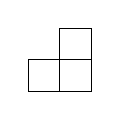
\begin{tikzpicture}[scale = 0.4]
		\draw (0,0)rectangle(1,1);
		\draw (1,0)rectangle(2,1);
		\draw (1,1)rectangle(2,2);
	\end{tikzpicture}
\end{center}
\vskip3mm
Riempire la griglia con i \textit{triomini}
\vskip3mm
Questo problema potrebbe sembrare un problema di backtracking, ma è molto più semplice.
\begin{itemize}
	\item L'idea è che si può dividere la griglia in 4
	\item Rimarrà dunque un buco in una delle 4 porzioni.
	\item Metto triomino in modo tale che sia a cavallo delle 3 porzioni senza buco
	\item Ho ottenuto ora 3 quadrati con lato \verb|n/2| con un posto occupato. Posso iterare ricorsivamente fino ad aver riempito tutta la griglia
\end{itemize}
\begin{center}
	\begin{tikzpicture}[scale = 0.4]
		\draw [thin, gray](0,0)grid(8,8);
		\draw [pattern = north west lines](2,2)rectangle(3,3);
		\draw [thick, white](2,0)--(2,8);
		\draw [thick, white](0,2)--(8,2);
		\draw [thick, dashed](2,0)--(2,8);
		\draw [thick, dashed](0,2)--(8,2);
		% \draw [thick, pattern = dots](1,1)--++(2,0)--++(0,1)--++(-1,0)--++(0,1)--++(-1,0)--cycle;
		\draw [thick](1,1)--++(2,0)--++(0,1)--++(-1,0)--++(0,1)--++(-1,0)--cycle;
	\end{tikzpicture}
\end{center}

\subsection{Knight tour}
Considerando che le mosse che può fare un cavallo sono le seguenti:
\begin{center}
	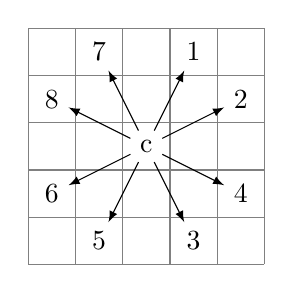
\begin{tikzpicture}[scale = 0.6]
		\draw [thin, gray](1,1)grid(6,6);
		\node (c)at (3.5,3.5)  {c};

		\draw (c)++(1,2)  node(1){1};
		\draw (c)++(2,1)  node(2){2};

		\draw (c)++(1,-2) node(3){3};
		\draw (c)++(2,-1) node(4){4};

		\draw (c)++(-1,-2)node(5){5};
		\draw (c)++(-2,-1)node(6){6};

		\draw (c)++(-1,2) node(7){7};
		\draw (c)++(-2,1) node(8){8};

		\draw [-latex](c) edge(1) edge(2) edge(3) edge(4) edge(5) edge(6) edge(7) edge(8);
	\end{tikzpicture}
\end{center}
\vskip3mm
si trovi un percorso di un cavallo su di una scacchiera che visiti ogni sua cella al massimo 1 volta.

\begin{itemize}
	\item Salvo in \verb|dp[i][j]| il passo a cui è stata visitata la cella \verb|(i,j)| o 0 se non è stata ancora visitata
	\item
	\item Per ogni posizione ho al massimo 8 opzioni, ossia il numero di mosse possibili per un cavallo
\end{itemize}

\begin{algoritmo}{Knight tour}
	\begin{algorithm}[H]
		\caption{Knight's Tour (Backtracking)}
		\SetKwFunction{KnightTour}{knightTour}
		\SetKwFunction{ProcessSolution}{processSolution}
		\SetKwFunction{Moves}{moves}
		\Fn{\Bool \KnightTour$(\Int[][]\ S,\ \Int\ i,\ \Int\ x,\ \Int\ y)$}{
		\Comment{\textcolor{mutedblue}{Se $i = 64$, ho fatto 63 mosse e ho completato un tour (aperto)}}\;
		\If{$i == 64$}{
			\ProcessSolution$(S)$\;
			\Return \textnormal{true}\;
		}
		\Set $C = \Moves(S, x, y)$\;
		\ForEach{$c \in C$}{
		$S[x][y] = i$\;
		\If{\KnightTour$(S, i + 1, x + m_x[c], y + m_y[c])$}{
		\Return \textnormal{true}\;
		}
		$S[x][y] = 0$\;
		}
		\Return \textnormal{false}\;
		}
	\end{algorithm}
\end{algoritmo}
Questo algoritmo esegue circa $  8^{63} \approx 7.84 \cdot  10^{55} $. Tantini
\subsection{Inviluppo convesso}
Dato un insimee di punti sul piano cartesiano, trovare il più piccolo poligono convesso che li contenga tutti e quanti.
\subsubsection{Algoritmo Naive}
\begin{itemize}
	\item Considero una retta per due punti $ a,b $
	\item Se tutti i restanti punti sono dalla stessa parte della retta allora per forza $ a $ e $ b $ appartengono al poligono ($ O\left(n\right) $)
	\item Ripeto per ogni coppia di punti ($ O\left(n^2 \right) $)
\end{itemize}
Complessità $ O\left(n^3\right) $

\subsubsection{Algoritmo di Jarvis}
Un approccio più intelligente sta nell'immaginarsi di "arrotolare" un bastoncino intorno all'ammasso di punti.
\begin{itemize}
	\item Considero il punto più a sinistra $ p $
	\item Considero l'inclinazione di ogni retta passante per $ p $ e $ x $ ($ O\left(n\right) $)
	\item Prendo la retta con angolo \textit{minore rispetto alla verticale}
	\item Setto $ t $ al punto della retta selezionata prima e itero ($ O\left(h\right) $, dove $ h $ è il numero di vertici del poligono finale)
\end{itemize}
Complessità $ O\left(nh\right) $, dove $ h $ è il numero di vertici del poligono finale.
\subsubsection{Algoritmo di Graham}
\begin{itemize}
	\item Seleziono punto con $ y $ minore. Lo chiamo $ p_1 $
	\item Ordino punti in base all'angolo che forma la retta per $ p_1 $ $ p $ rispetto all'orizzontale
	\item Inserisco $ p_1 $  e $ p_2 $ in uno stack.Chiamo $ p $ il punto corrente. Considero la retta formata fra gli ultimi due punti inseriti nello stack
	      \begin{itemize}
		      \item  Se $ p_1 $ e $ p $ stanno nello stesso semipiano delineato dalla retta inserisco $ p $ nello stack
		      \item Altrimenti elimino punti dallo stack e ripeto il controllo finché questo non è vero
	      \end{itemize}
\end{itemize}
Siccome ogni punto viene inserito e rimosso al più una volta dallo stack, il costo dell'algoritmo è $ O\left(n\right) $. Tuttavia i punti vanno ordinati, dunque il costo finale è $ O\left(n \log n\right) $.
\vskip3mm
\begin{algoritmo}{Grahams inviluppo convesso}
	\begin{algorithm}[H]
		\caption{Graham's Scan Algorithm (Convex Hull - Stack Implementation)}
		\SetKwFunction{Graham}{graham}
		\SetKwData{Point}{point}
		\SetKwFunction{Top2}{top2}
		\SetKwFunction{SameSide}{same\_side}

		\Fn{\Stack \Graham$(\Point[]\ p,\ \Int\ n)$}{
			\Stack $S = \Stack()$\;
			$S.\Push(p_1); S.\Push(p_2)$\;
			\For{$i = 3$ \KwTo $n$}{
				\While{\KwNot \SameSide$(S.\Top(), S.\Top2(), p_1, p_i)$}{
					$S.\Pop()$\;
				}
				$S.\Push(p_i)$\;
			}
			\Return $S$\;
		}
	\end{algorithm}
\end{algoritmo}
\section{Algoritmi probabilitstici}
Possiamo distinguere tra due tipi di algoritmi probabilistici:
\begin{itemize}
	\item Algoritmi di Montecarlo: il risultato è corretto solo una  \%  delle volte
	\item Algoritmi di Las Vegas: il risultato è corretto sempre, ma il tempo di esecuzione è probabilistico
\end{itemize}
\subsection{Test di primalità}
Dato in input un numero $ n $, determinare se p primo.

\subsubsection{Varsione naif}
Per ogni numero fino alla $ \sqrt{n} $ controllo se è divisibile
\vskip3mm
\begin{algoritmo}{Prime check naif}
	\begin{algorithm}[H]
		\caption{Prime Check (Naive Implementation)}
		\SetKwFunction{IsPrimeNaif}{isPrimeNaif}
		\Fn{\Bool \IsPrimeNaif$(\Int\ n)$}{
			\For{$i = 2$ \KwTo $\lfloor \sqrt{n} \rfloor$}{
				\If{$n / i == \lfloor n / i \rfloor$}{
					\Return \textnormal{false}\;
				}
			}
			\Return \textnormal{true}\;
		}
	\end{algorithm}
\end{algoritmo}

\subsubsection{Versione di fermat}
Il piccolo teorema di Fermat afferma che:
\begin{teorema}{Piccolo teorema di Fermat}
	Se un numero $ n $ è primo, allora:
	\[
		\forall b \in \left[2, n\right) \quad b^{n-1} \mod n  = 1
	\]
\end{teorema}
\vskip3mm
\begin{algoritmo}{Prime check Fermat}
	\begin{algorithm}[H]
		\caption{Probabilistic Prime Check (Fermat's Test)}
		\SetKwFunction{IsPrimeFermat}{isPrimeFermat}
		\Fn{\Bool \IsPrimeFermat$(\Int\ n)$}{
			\For{$i = 1$ \KwTo $k$}{
				$b = \textnormal{random}(2, n - 1)$\;
				\If{$b^{n-1} \bmod n \neq 1$}{
					\Return \textnormal{false}\;
				}
			}
			\Return \textnormal{true}\;
		}
	\end{algorithm}
\end{algoritmo}
Se questo algoritmo ritorna
\begin{itemize}
	\item \verb|false| allora $ n $ è sicuramente composto (\textit{non primo})
	\item \verb|true| allora $ n $ può essere sia primo che non
\end{itemize}
Non ho garanzie sulla probabilità con cui azzecco il risultato

\subsubsection{Algoritmo di Miller-Rabin}
\begin{teorema}{Teorema di Miller-Rabin}
	Se $n$ è primo e ho:
	\begin{enumerate}
		\item $ b \in \left[2, n\right) $
		\item $n - 1 = m \cdot 2^v$, $m$ dispari.
	\end{enumerate}
	alora per ogni $b$:

	\begin{enumerate}
		\item $\text{mcd}(n, b) = 1$
		\item $b^m \mod n = 1 \lor \exists i, 0 \leq i < v : b^{m \cdot 2^i} \mod n = n - 1$
	\end{enumerate}
\end{teorema}\label{teo-miller-rabin}
Nota come posso scrivere $ m\cdot 2^{v} $ in binario. $ v $ è il numero di \textit{trailing zeros} se scriviamo il numero in binario
\[
	\underbracket[0.1ex]{1001011}_{m}\underbracket[0.1ex]{000}_{v}
\]

Di base per controllare mi basta verificare queste due condizioni. Se trovo un valore di $ b $ (\textit{testimone}) per cui non è rispettata la 1 oppure non esiste un valore di $ i $ per cui è rispettata la 2 sono \textit{sicuro} che il  numero \underline{non} sia primo. Queste sono
\begin{center}
	\underline{condizioni necessarie ma non sufficienti} per la primalità
\end{center}

\begin{algoritmo}{Prime check Miller-Rabin}
	\begin{algorithm}[H]
		\caption{Probabilistic Prime Check}
		\SetKwFunction{IsPrime}{isPrime}
		\Fn{\Bool \IsPrime$(\Int\ n)$}{
			\For{$i = 1$ \KwTo $k$}{
				$b = \textnormal{random}(2, n - 1)$\;
				\If{\textnormal{isComposite}$(n, b)$}{
					\Return \textnormal{false}\;
				}
			}
			\Return \textnormal{true}\;
		}
	\end{algorithm}
\end{algoritmo}
\verb|isComposite(n,b)| esegue un check secondo il teorema descritto \hyperref[teo-miller-rabin]{qui}.
\vskip3mm
Si può dimostrare che se $ n $ è composto si esistono almento $ \frac{3}{4} \cdot (n-1) $ testimoni. Quindi ho $ \frac{1}{4} $ di possibilità di sbagliare. Eseguendo $ k $ passate ho $ \frac{1}{4}^{k} $ possibilità di errare, ossia pochissime
\vskip3mm
Complessità: $ O(k \log^2 n \log \log n \log \log \log n) $ (\textit{fanculo la dimostrazione})
\subsection{Espressione polinomiale nulla}
\begin{teorema}{Annullamento polinomiale}
	Se ogni $ v_i $ è un valore intero compreso casuale fra $ 1 $ e $ 2d $, dove $ d $ è il grado del polinomio, allora la probabilità di errore non supera 1/2.
\end{teorema}

L'idea è di valutare $ k $ volte il polinomio in valori presi a caso.
\begin{itemize}
	\item Se \textit{si annulla}: il polinomio può essere identicamente nullo oppure no
	\item Se \textit{non si annulla}: il polinomio \textit{non} può essere identicamente nullo
	\item Probabilità di errore $ \left(\frac{1}{2}\right)^{k} $
\end{itemize}
\subsection{Bloom filter}
Struttura dati probabilistica che funziona come hashmap ma eseguendo \verb|contains(i)|:
\begin{itemize}
	\item Se \verb|i| \textit{non è contenuto} $ \rightarrow  $ ritorna \verb|false|
	\item Se \verb|i|  \textit{è contenuto} $ \rightarrow  $ ritorna \verb|true o false|
\end{itemize}
Le funzioni sono le seguenti:
\begin{itemize}
	\item \verb|insert(i)|: ho $ n $ funzioni hash. Per ogni funzione setto a $ 1 $ il bit corrispondente
	\item \verb|contains(i)|: ritorna \verb|true| se tutti i bit corrispondendi alle funzioni hash sono 1, false altrimenti
\end{itemize}
Si può dimostrare che la efficienza di questa struttura segue quanto descritto da queste formule:
\begin{itemize}
	\item Dati $n$ oggetti, $m$ bit, $k$ funzioni hash, la probabilità di un falso positivo è pari a:
	      \[
		      \epsilon = \left( 1 - e^{-kn/m} \right)^k
	      \]

	\item Dati $n$ oggetti e $m$ bit, il valore ottimale per $k$ è pari a:
	      \[
		      k = \frac{m}{n} \ln 2
	      \]

	\item Dati $n$ oggetti e una probabilità di falsi positivi $\epsilon$, il numero di bit $m$ richiesti è pari a:
	      \[
		      m = -\frac{n \ln \epsilon}{(\ln 2)^2}
	      \]
\end{itemize}


\forestset{box/.style={
draw, no edge, l=0, l sep=1.5ex,
calign=first, anchor=base west,
content format={\strut\forestoption{content}},
if n children=0{}{
after packing node={
minimum width/.pgfmath=
	{s("!l")+max_x("!l")-s("!1")-min_x("!1")},
for children/.wrap pgfmath arg={s+={##1}}{0},
typeset node}}}}


\subsection{Selezione naif}
\begin{algoritmo}{Selezione naif}
	\begin{algorithm}[H]
		\caption{Selection naif}
		\SetKwFunction{NaifSelect}{naifSelect}
		\SetKwFunction{Sort}{sort}
		\Fn{\Int \NaifSelect$(\Item[]\ A,\ \Int\ n,\ \Int\ k)$}{
			\Sort$(A)$\Comment*[r]{$ O(n \log n) $}
			\Return $A\left[k\right]$\;
		}
	\end{algorithm}
\end{algoritmo}
Questo approccio ha complessità $ O \left(n \log n\right) $

\subsection{Selezione simil heapsort}
\begin{algoritmo}{Selezione simil Heap-sort}
	\begin{algorithm}[H]
		\caption{Heap Selection}
		\SetKwFunction{HeapSelect}{heapSelect}
		\SetKwFunction{DeleteMin}{deleteMin}
		\SetKwFunction{BuildHeap}{buildHeap}
		\Fn{\Int \HeapSelect$(\Item[]\ A,\ \Int\ n,\ \Int\ k)$}{
			\BuildHeap$(A)$\Comment*[r]{$ O(n) $}
			\For{$i = 1$ \KwTo $k - 1$}{
				\DeleteMin$(A, n)$\Comment*[r]{$ O(\log ) $}
			}
			\Return \DeleteMin$(A, n)$\;
		}
	\end{algorithm}
\end{algoritmo}
Questo approccio ha complessità $ O \left(n + k \log n\right) $

\subsection{Selezione probabilistica}
Posso avere un algoritmo probabilistico in stile \textit{quicksort}.
\begin{itemize}
	\item Scelgo un pivot a caso
	\item Metto alla sua sinistra tutti gli elementi $ < $ pivot
	\item Chiamo ricorsivamente \textit{solo} sulla parte di mio interesse (\textit{è qua la differenza rispetto al \hyperref[quicksort]{quicksort}}, che invece chiama l'algoritmo su entrambe)
\end{itemize}
\begin{algoritmo}{Selezione probabilistica}
	\begin{algorithm}[H]
		\caption{Selection Algorithm}
		\SetKwFunction{Selection}{selection}
		\SetKwFunction{Pivot}{pivot}
		\Fn{\Item \Selection$(\Item[]\ A,\ \Int\ start,\ \Int\ end,\ \Int\ k)$}{
			\If{$start == end$}{
				\Return $A[start]$\;
			}
			\Else{
				\Int $j = \Pivot(A, start, end)$\;
				\Int $q = j - start + 1$\;
				\If{$k == q$}{
					\Return $A[j]$\;
				}
				\ElseIf{$k < q$}{
					\Return \Selection$(A, start, j - 1, k)$\;
				}
				\Else{
					\Return \Selection$(A, j + 1, end, k - q)$\;
				}
			}
		}
	\end{algorithm}
\end{algoritmo}
La funzione \verb|pivot| prende gli elementi in \verb|[start, end]|, e mette tutti gli elementi \verb|< v[start]| a sinistra e i rimanenti a destra. Di base usa \verb|a[start]| come pivot e \underline{sposta gli elementi}
\subsubsection{Complessità}
Assumiamo di dover sempre chiamare ricorsivamente \verb|select| sulla porzione di vettore più lunga(caso pessimo).
Assumiamo che \verb|pivot()| restituisca con la stessa probabilità una qualsiasi posizione $j$ del vettore $A$

\[
	T(n)=n+\underbracket[0.1ex]{\frac{1}{n} \sum_{q=1}^n T(\max \{q-1, n-q\})}_{\text{media su tutti i casi possibili}}
\]
Ad esempio, su $ n = 4 $ posso avere i seguenti modi di spezzare il vettore e la chiamata ricorsiva sarebbe effettuata sulla porzione in rosso:
\[
	\left\{0,\textcolor{mutedred}{4}\right\}, \left\{1,\textcolor{mutedred}{3}\right\}, \left\{\textcolor{mutedred}{2},2\right\}, \left\{\textcolor{mutedred}{3},1\right\}, \left\{\textcolor{mutedred}{4},0\right\}
\]
Quindi ogni chiamata è limitata superiormente dalla somma fino a $ \frac{n}{2} $ diviso $ n $
\[
	T\left(n\right) \le n + \frac{1}{n} \sum_{q = \left\lfloor \frac{n}{2} \right\rfloor}^{n-1} 2T\left(q\right)
\]
Posso procedere per sostituzione  \hyperref[complessita per sostituzione]{sostituzione}
\vskip3mm

\begin{align*}
	T(n) & \leq n+\frac{1}{n} \sum_{q=\lfloor n / 2\rfloor}^{n-1} 2 \cdot c q \leq n+\frac{2 c}{n} \sum_{q=\lfloor n / 2\rfloor}^{n-1} q &  & \text{Sostituzione, raccolgo } 2 c            \\
	     & =n+\frac{2 c}{n}\left(\sum_{q=1}^{n-1} q-\sum_{q=1}^{\lfloor n / 2\rfloor-1} q\right)                                         &  & \text{Sottrazione prima parte}                \\
	     & =n+\frac{2 c}{n} \cdot\left(\frac{n(n-1)}{2}-\frac{(\lfloor n / 2\rfloor)(\lfloor n / 2\rfloor-1)}{2}\right)                                                                     \\
	     & \leq n+\frac{2 c}{n} \cdot\left(\frac{n(n-1)}{2}-\frac{(n / 2-1)(n / 2-2)}{2}\right)                                          &  & \text{Rimozione limite inferiore}             \\
	     & =n+\frac{c}{n} \cdot \frac{\left(n^2-n-\left(1 / 4 n^2-3 / 2 n+2\right)\right)}{1}                                                                                               \\
	     & =n+c / n \cdot\left(3 / 4 n^2+1 / 2 n-2\right)                                                                                                                                   \\
	     & \leq n+c / n \cdot\left(3 / 4 n^2+1 / 2 n\right) = n+3 / 4 c n+1 / 2 c n                                                      &  & \text{Vera per } c \geq 6 \text{ e } n \geq 1
\end{align*}
Quindi la complessità media è $ O\left(n\right) $





\subsection{Selezione deterministica}
L'idea è che se ho la certezza di scegliere il pivot in modo tale che non taglio solo il primo elemento, la formula ricorsiva è di
\begin{center}
	\begin{tikzpicture}[scale = 0.4]
		\draw (0,0) grid (10,1);
		\draw (0,-2) grid (10,-1);

		\node [anchor = west] at (10.5,0.5) {$ T\left(n\right) = T \left(n-1\right) $};
		\node [anchor = west] at (10.5,-1.5) {$ T\left(n\right) = T \left(\frac{n}{k}\right) $};

		\draw [thick, white](1,-0.2)--++(0,1.4);
		\draw [thick, white](6,-2.2)--++(0,1.4);

		\draw [thick, dashed, mutedred](1,-0.2)--++(0,1.4);
		\draw [thick, dashed, mutedred](6,-2.2)--++(0,1.4);
	\end{tikzpicture}
\end{center}


L'idea di base è che scegliendo un pivot che è la mediana fra le mediane dei gruppi da 5, ho la garanzia di avere $ \frac{7}{10}n $ degli elementi a destra/a sinistra del pivot. Quindi non spezzero mai in stile $ T\left(n\right) = T\left(n-1\right) $. La dimostrazione è questa:
\begin{itemize}
	\item Ogni mediana di un blocco di 5 ha alla sua sinistra 3 interi minori (\textit{inclusa la mediana stessa})
	\item La mediana delle mediane ha alla sua sinistra esattamente $  \frac{n}{5} / 2 $ mediane per lo stesso ragionamento di prima
	\item Quindi alla sinistra della mediana delle mediane ci devono essere
	      \[
		      \text{elementi minori} = 3 \cdot \frac{n}{5} / {2} = \frac{3}{10}n
	      \]
	\item Assumo di selezionare sempre la parte peggiore, ossia la porzione larga $ \frac{7}{10}n $
\end{itemize}
Quindi, siccome ad ogni chiamata ricorsiva avrò $ T\left(n\right) = T\left(\frac{3}{7}n\right) $, l'algoritmo è lineare per il \hyperref[master theorem]{master theorem}

\vskip3mm

\begin{algoritmo}{Selezione deterministica}
	\begin{algorithm}[H]
		\caption{Selezione Deterministica}
		\SetKwFunction{Select}{select}
		\SetKwFunction{InsertionSort}{InsertionSort}
		\SetKwFunction{MedianFive}{median5}
		\SetKwFunction{Pivot}{pivot}
		\Fn{\Item \Select$(\Item[]\ A,\ \Int\ start,\ \Int\ end,\ \Int\ k)$}{

			\Comment{Sotto una certa dimensione trovo mediana tramite sort in $ O\left(1\right) $}
			\If{$end - start + 1 \leq 10$}{
				\InsertionSort$(A, start, end)$ \Comment{Versione con indici inizio/fine}
				\Return $A[start + k - 1]$\;
			}
			\vskip5mm

			\Comment{Divide array in sottovett di dim 5 e calcola la mediana}
			$\Int[]\ M = \textnormal{new int}[1 \dots \lceil n / 5 \rceil]$\;
			\For{$i = 1$ \KwTo $\lceil n / 5 \rceil$}{
				$M[i] = \MedianFive$(A, start + (i - 1) $\cdot$ 5, end)\;
			}

			\vskip5mm
			\Comment{Individua la mediana delle mediane e usala come perno}
			\Item $m = \Select(M, 1, \lceil n / 5 \rceil, \lceil \lceil n / 5 \rceil / 2 \rceil)$\Comment*[r]{\textcolor{mutedred}{Chiamata 1}}
			\Int $j = \Pivot$(A, start, end, m) \Comment*[r]{Usa $ m $ come elemento pivot}

			\vskip5mm
			\Comment{Calcola l'indice q di m in [start...end]}
			\Int $q = j - start + 1$\;
			\If{$q == k$}{
				\Return $m$\;
			}
			\ElseIf{$q < k$}{
				\Return \Select$(A, start, q - 1, k)$\Comment*[r]{\textcolor{mutedred}{Chiamata 2}}
			}
			\Else{
				\Return \Select$(A, q + 1, end, k - q)$\Comment*[r]{\textcolor{mutedred}{Chiamata 3}}
			}
		}
	\end{algorithm}
\end{algoritmo}
Complessità:
\[
	T\left(n\right) = \underbracket[0.1ex]{T\left(\frac{n}{5}\right)}_{\text{chiamata 1}} +  \underbracket[0.1ex]{T \left(\frac{7}{10}n\right) }_{\text{chiamata 2 o 3}}+ \underbracket[0.1ex]{\frac{11}{5} n}_{\text{mediane pivot $^{*} $}}
\]
$ ^{*} $ il fattore deriva da 
\begin{itemize}
  \item $ 6 \cdot \frac{n}{5} $ per trovare mediane di blocchetti da 5
  \item $ n $ per eseguire l'operazione di \verb|pivot| sull'array originale
\end{itemize}

Risolvendo la ricorrenza si può verificare che la complessità è di $ O\left(n\right) $

\begin{forest}
	for tree={draw, grow = -90, sibling distance=1mm, level distance=1mm, box, inner ysep=0, s sep = 1}
	[
	[
			[
					[]
						[]
						[]
						[]
						[]
				]
				[
					[]
						[]
						[]
						[]
						[]
				]
				[
					[]
						[]
						[]
						[]
						[]
				]
				[
					[]
						[]
						[]
						[]
						[]
				]
				[
					[]
						[]
						[]
						[]
						[]
				]
		]
		[
			[
					[]
						[]
						[]
						[]
						[]
				]
				[
					[]
						[]
						[]
						[]
						[]
				]
				[
					[]
						[]
						[]
						[]
						[]
				]
				[
					[]
						[]
						[]
						[]
						[]
				]
				[
					[]
						[]
						[]
						[]
						[]
				]
		]
	]
\end{forest}
\section{Problemi np completi}
Possiamo distinguere tra 3 tipi di problemi:
\begin{itemize}
	\item Problemi di \textit{ottimizzazione}: trova la soluzione migliore
	\item Problemi di \textit{ricerca}: trova una possibile soluzione
	\item Problemi di \textit{decisione}: verifica se una soddisfa certi prerequisiti
\end{itemize}
Nota bene che

\begin{center}
	Si sa risolve efficientemente un problema di \textit{ottimizzazione}
	\[
		\Rightarrow
	\]
	Si sa risolve efficientemente un problema di \textit{decisione}
\end{center}
\subsection{Riduzione polinomiale}
\begin{definizione}{Riduzione polinomiale}
	Se posso risolvere un problema $ P_1 $ con l'algoritmo risolutivo di un problema $ P_2 $, convertendo l'input/output di $ P_1 $ in tempo \textit{polinomiale} si dice che $ P_1 $ è riducibile polinialmente a $ P_2 $
\end{definizione}
Vediamo ora una serie di problemi $ NP $ complessi che possono essere ridotti fra di loro

\subsection{Colorazione dei grafi}\label{problema colorazione}
Dato un grafo non orientato colorare i suoi vertici con $ k $ colori in modo che non ci siano vertici adiacenti con lo stesso colore
\begin{itemize}
	\item \textit{Ottimizzazione}: trovare il numero minore di colori $ k $
	\item \textit{Decisione}: esiste una colorazione valida per $ k $
\end{itemize}

\subsection{Sudoku}
Data una griglia $ n^2 x n^2  $ riempirla con numeri da $ 1\ldots n^2  $ secondo le regole del sudoku
\vskip3mm
Il prolema del sudoku è \textit{riducibile polinomialmente} al problema di \hyperref[problema colorazione]{colorazione dei grafi}.
\begin{center}
	\begin{tikzpicture}
		\draw (0,0)grid(9,9);
		\draw [thick](3,0)--++(0,9);
		\draw [thick](6,0)--++(0,9);
		\draw [thick](0,3)--++(9,0);
		\draw [thick](0,6)--++(9,0);
		\begin{scope}[shift ={(-0.5, -0.5)}]
			\node [whitedot] (start)at (1,9){$ a $};
			\draw [bend right,dashed, ->](start)
			edge(1,1)
			edge(1,2)
			edge(1,3)
			edge(1,4)
			edge(1,5)
			edge(1,6)
			edge(1,7)
			edge(1,8);
			\draw [bend left,dashed, ->](start)
			edge(2,9)
			edge(3,9)
			edge(4,9)
			edge(5,9)
			edge(6,9)
			edge(7,9)
			edge(8,9)
			edge(9,9);
			\draw [dashed, ->](start)
			edge (2,8)
			edge (3,8)
			edge (2,7)
			edge (3,7);
		\end{scope}
	\end{tikzpicture}
\end{center}
Supponendo di costruire un grafo in cui ogni cella del sudoku e collegata con le colonne e con gli elementi della cella interna, facendo il coloring del grafo non posso dare lo stesso colore (numero) a questi elementi
\subsection{Insieme indipendente e vertex cover}\label{insieme indipendente}
\begin{definizione}{Insieme indipendente}
	Dato un grafo non orientato, un \textit{insieme indipendete} è un insieme di vertici per cui non ce nessun \textit{arco} fra due nodi di questo insieme
\end{definizione}
\begin{definizione}{Vertex cover}
	Dato un grafo non oeirnetato, una \textit{vertex cover} è un insieme di vertici tale che ogni arco del grafo ha almeno un estremo in questo insieme
\end{definizione}
\begin{teorema}{Dualità insieme indipendente e vertex cover}
	Se $ S $ è un insieme indipendente e $ V $ l'indieme di vertici del grafo, allora $ V-S $ è una vertex cover
\end{teorema}
\subsubsection{Dimostrazione}
\begin{itemize}
	\item Sia $ S $ un insieme indipendente. Allora ogni altro arco o ha $ 1 $ estremo in $ V-S $ se l'altro è in $ S $, oppure li ha entrambi
	\item Sia $ S $ una vertex cover. Se $ V-S $ non fosse indipendere allora ci sarebbe un arco con entrambi gli estremi in $ V-S $. Questo arco tuttavia avendo entrambi gli estremi in $ V-S $, non ne ha in $ S $, quindi $ S $ non può essere vertex cover
\end{itemize}
\subsection{Formule booleane in forma normale congiuntiva}
\begin{definizione}{Formule booleane in forma normale congiuntiva}
	Una formula booleana in forma normale congiunta è un'insieme di letterali (che possono esser \verb|true| o \verb|false|). I letterali sono uniti da \verb|and|($ \land $) fra gruppi di \verb|or| ($ \lor $)
	\[
		(x \lor \overline{y} \lor z) \land (\overline{x} \lor w) \land y
	\]
\end{definizione}
Il problema principale è quello della \textit{satisfiability}:
\begin{itemize}
	\item \textit{Satisfiability}: esiste una combinazioni di valori che rendono la formula vera
	\item \textit{3-satisfiability}: ogni clausula è data da esattamente 3  letterali (es $ x \lor \overline{z} \lor z $)
\end{itemize}\label{satisfiability}
\begin{teorema}{Riducibilità polinomiale satisfiability}
	Il problema di satisfiability è riducibile polinomialmente come segue:
	\[
		\text{SAT} \leq_p \text{3-SAT} \leq_p \text{INDEPENDENT-SET} \leq_p \text{VERTEX-COVER}
	\]
\end{teorema}
\subsubsection{Dimostrazione}
$ \text{SAT} \leq_p \text{3-SAT} $
\begin{itemize}
	\item Se la clausola è più lunga di tre elementi, si introduce una nuova variabile e si divide la clausola in due:
	      \[
		      (a \lor b \lor c \lor d) \equiv (a \lor b \lor z) \land (\overline{z} \lor c \lor d)
	      \]
	      l'idea è che una variabile $ z $ fa da "switch", accendendo il blocco a sinistra o il blocco a destra
	\item Se la clausola è più corta di tre elementi, si fa "padding":
	      \[
		      (a \lor b) \equiv (a \lor a \lor b)
	      \]
\end{itemize}
$ \text{3-SAT} \leq_p \text{INDEPENDENT-SET} $
\begin{itemize}
	\item Se costruisco un grafo come mostrato \hyperref[3-sat graph]{qui}
	      \begin{itemize}
		      \item Collego ogni letterale con ogni corrispondente negato
		      \item Collego ogni letterale con ogni letterale della stessa clausula
	      \end{itemize}
	\item L'idea è che se seleziono un letterale (lo rendo \verb|true|), non posso più prenderne nella stessa clausula e non posso avverare i suoi negati
	\item Se ne trovo $ k $, che sono per forza in $ k $ clausule separate, ho avverato ogni clausula
\end{itemize}

\begin{figure}[H]
	\begin{center}
		\begin{tikzpicture}
			% First triangle
			\node (1) at (0,0) {$x$};
			\node (2) at (2,0) {$\overline{y}$};
			\node (3) at (1,1.5) {$z$};

			% Second triangle
			\begin{scope}[shift={(4,0)}]
				\node (4) at (0,0) {$\overline{x}$};
				\node (5) at (2,0) {$\overline{y}$};
				\node (6) at (1,1.5) {$\overline{z}$};
			\end{scope}

			% Third triangle
			\begin{scope}[shift={(8,0)}]
				\node (7) at (0,0) {$\overline{x}$};
				\node (8) at (2,0) {$y$};
				\node (9) at (1,1.5) {$z$};
			\end{scope}

			% Edges for the first triangle
			\draw[dashed, mutedred] (1) -- (2);
			\draw[dashed, mutedred] (2) -- (3);
			\draw[dashed, mutedred] (3) -- (1);

			% Edges for thmutede second triangle
			\draw[dashed, mutedred] (4) -- (5);
			\draw[dashed, mutedred] (5) -- (6);
			\draw[dashed, mutedred] (6) -- (4);

			% Edges for thmutede third triangle
			\draw[dashed, mutedred] (7) -- (8);
			\draw[dashed, mutedred] (8) -- (9);
			\draw[dashed, mutedred] (9) -- (7);

			% Blue edges connecting triangles
			\draw[bend left] (3) to (6);
			\draw[bend left] (3) to (9);
			\draw[bend left] (6) to (9);
			\draw[bend right] (1) to (5);
			\draw[bend right] (1) to (7);
			\draw[bend right] (2) to (4);
			\draw[bend right] (2) to (8);
			\draw[bend right] (5) to (7);
			\draw[bend right] (4) to (8);
		\end{tikzpicture}
	\end{center}
	\caption{3-sat graph}
	\label{3-sat graph}
\end{figure}

\subsection{Classi di problemi}
\begin{definizione}{Classi di complessità}
	Data una qualunque funzione $f(n)$, chiamiamo:
	\begin{itemize}
		\item $\mathbb{TIME}(f(n))$ l'insieme dei problemi decisionali risolvibili da un algoritmo che lavora in tempo $O(f(n))$
		\item $\mathbb{SPACE}(f(n))$ gli insiemi dei problemi decisionali risolvibili da un algoritmo che lavora in spazio $O(f(n))$.
	\end{itemize}
\end{definizione}


\begin{definizione}{Classi $\mathbb{P, PSPACE}$}
	Classe $ \mathbb{P} $\\
	La classe $ \mathbb{P} $ è la classe dei problemi decisionali risolvibili in tempo polinomiale nella dimensione $n$ dell'istanza di ingresso:
	\[
		\mathbb{P} = \bigcup_{c=0}^{\infty} \mathbb{TIME}(n^c)
	\]
	\vskip3mm
	Classe $ \mathbb{PSPACE} $\\
	La classe $ \mathbb{PSPACE} $ è la classe dei problemi decisionali risolvibili in spazio polinomiale nella dimensione $n$ dell'istanza di ingresso:
	\[
		\mathbb{PSPACE} = \bigcup_{c=0}^{\infty} \mathbb{SPACE}(n^c)
	\]
\end{definizione}
Nota che se un problema è $ \mathbb{PSPACE} $ allora è anche $ \mathbb{P} $. In qualche modo dovro "iterare" tutta la soluzione

\begin{definizione}{Certificato}\label{certificato}
	Informalmente, un certificato  è una "soluzione ammissibile" la cui ottimalità può essere dimostrata in tempo polinomiale.
	\vskip3mm
	Formalmente, dato un problema decisionale $ R $ e un suo input $ I $ che si sa essere vero, un certificato è un insieme di dati che permettono di provare che $ \left(i, \text{\ttfamily{true}}\right) \in R $
\end{definizione}
Ad edempio un assegnamento di verità alle variabili della formula SAT
\begin{definizione}{Classe $ \mathbb{NP} $}
	L’insieme di tutti i problemi che ammettono un \hyperref[certificato]{certificato} verificabile in tempo polinomiale.
\end{definizione}
Non tutti i certificati sono verificabili in tempo polinomiale. Ad esempio se prendo il problema di \hyperref[satisfiability]{satisfiability} e lo estendo con i quantificatori universali (invece di chiedermi se esista un valore di $ x $ che la avvera, mi chiedo se sia vera \textit{per ogni} $ \forall  x$ ).

\begin{definizione}{Problema \textit{NP-arduo} (\textit{NP-hard})}
	Un problema decisionale $R$ si dice \textit{NP-arduo} se ogni problema $Q \in \text{NP}$ è riducibile polinomialmente a $R$ ($Q \leq_p R$).
\end{definizione}

\begin{definizione}{Problema \textit{NP-completo} (\textit{NP-complete})}
	Un problema decisionale $R$ si dice \textit{NP-completo} se appartiene alla classe \textit{NP} ed è \textit{NP-hard}.
\end{definizione}

Dimostrare che un problema è $ NP-completo $ è difficilissimo. Ad oggi abbiamo solo:
\begin{teorema}{Teorema di Cook-Levin}
	Cook Levin ha dimostrato che il problema di \textit{SAT} $ \mathbb{NP} $-completo
\end{teorema}
\begin{definizione}{Dimensione di un problema}
	La dimensione di un problema è il numero di bit necessari a rappresentare un'istanza del problema.
	\begin{itemize}
		\item $ d $: \textit{dimensione}, ossia numero di bit per rappresentare l'intero problema
		\item \#: valore \textit{numerico} dell'intero \textit{più grande} in input
	\end{itemize}
\end{definizione}

\begin{definizione}{Problema fortemente/debolmente NP-completo}
	Sia $ R_{pol} $ la \textit{versione ridotta} di un problema, ottenuta limitando la dimensione dell'intero maggiore \# superiormente:
	\[
		\text{\#} = O\left(n^{c}\right)
	\]
	allora
	\begin{itemize}
		\item   Se $ R_{pol} $ rimane $ \mathbb{NP} $-completo, allora $ R $ è detto \textit{fortemente NP-completo}.
		\item   Se $ R_{pol} $ diventa di complessità polinomiale $ \mathbb{P} $, allora $ R $ è detto \textit{debolmente NP-completo}.
	\end{itemize}
\end{definizione}
L'idea intuitiva è che se limitando la velocità con cui cresce l'input riusciamo ad ottenere complessità polinomiale, il problema è debolmente \textit{NP-completo}
\subsubsection{Esempio base}
Supponi di avere un problema che prende in input un singolo numerale $ k = 2^{t} $, con complessità $ O\left(k\right) $. Se esprimo la complessità in funzione del \textit{numero di bit} necessari per rappresentare l'input, allora
\[
	\text{complessità} = O\left(2^{k}\right)
\]
se limito superiormente la dimensione dei numerali ($ k $) il problema diventa polinomiale. In particolare, la dimensione dei numerali deve essere al più polinomiale nella dimensione del problema
\[
	k = O\left(t^{c}\right) \Rightarrow  \text{complessità} = O\left(k\right) = O\left(O\left(t^{c}\right)\right) = O\left(t^{c}\right)
\]
\subsubsection{Subset sum}
Complessità $ O\left(nk\right) $. Debolmente \textit{NP-completo}
\vskip3mm
se $ k = O\left(n^{c}\right) $  allor
\[
	\text{Complessità} = O\left(n^{c} \cdot n\right) = O\left(n^{c+1}\right)
\]

\subsubsection{Clique}
Complessità $ O\left(n^{2}\right) $. Fortemente \textit{NP-completo}
\vskip3mm
Limitare superiormente $ k $ non ha effetto in quanto è gia limitata superiormente. Se $ k > n $ per forza la risposta è \verb|true|

\subsubsection{Esempi debolmente vs fortemente NP-completo}
\begin{itemize}
	\item \textit{Subset sub}: limitando la dimensione di $ k  \rightarrow k = O\left(n^{c}\right)$ (la somma da raggiongere) ottengo complessità polinomiale
	      \[
		      \text{Complessità} = O\left(nk\right) = O \left(n \cdot  O\left(n^{c}\right)\right) = O \left(n^{c+1}\right)
	      \]
	\item \textit{Clique (cricca)}: limitare l'input $ k $ non ha effetto in quanto è già limitato superiormente da $ n $ (se $ k>n $ per forza non vi sono soluzioni). La versione ridotta del problema è dunque uguale a quella non ridotta
	      i
\end{itemize}
\section{Soluzioni a problemi intrattabili}
% Dato un vettore \verb|v|, determinare se esiste un insieme di suoi elementi la cui somma sia uguale a \verb|k|
% \vskip3mm
% Abbiamo visto la versione di ricerca \hyperref[subset sum]{qui}, ora vediamo la ersione decisionale.
% Definiamo una tabella booleana $DP[0 \dots n][0 \dots k]$.
% \subsubsection{Soluzione}
% Uso prog dinamica. $DP[i][r]$ è uguale a \textbf{true} se esiste un sottoinsieme dei primi $i$ valori memorizzati in $A$ la cui somma è pari a $r$, \textbf{false} altrimenti.
% \begin{itemize}
% 	\item Se $ A\left[i\right] $ non ci sta nella somma da riempire allora lo riempio senza l'elemento \textit{i-esimo}
% 	      \[
% 		      DP[i-1][r]
% 	      \]
% 	\item Se $ A\left[i\right] $ ci sta nella somma da riempire allora vedo se riesco a riempirlo con o senza l'element
% 	      \textit{i-iesimo}
% 	      \[
% 		      DP[i-1][r] \lor DP[i-1][r - A[i]]
% 	      \]
% \end{itemize}
% \[
% 	DP[i][r] =
% 	\begin{cases}
% 		\text{true}                       & r = 0                               \\
% 		\text{false}                      & r > 0 \land i = 0                   \\
% 		DP[i-1][r]                        & r > 0 \land i > 0 \land A[i] > r    \\
% 		DP[i-1][r] \lor DP[i-1][r - A[i]] & r > 0 \land i > 0 \land A[i] \leq r
% 	\end{cases}
% \]

Spesso dobbiamo accontentarci di una soluzione approssimata per un problema di ottimizzazione.
\begin{definizione}{$\alpha\left(n\right) $ approssimazione di un problema}
	Un problema si dice essere $ \alpha \left(n\right) $ approssimato se la soluzione dista al massimo $ \alpha\left(n\right) $ dalla soluzione ottimale. Detto $ c\left(n\right) $ il costo della soluzione trovata e $ c\left(x^{*}\right) $ il costo della soluzione ideale, allora
	\[
		c\left(x\right) \leq c\left(x^{*}\right) \cdot \alpha\left(n\right)
	\]
\end{definizione}
\subsection{Bin packing}
Supponiamo di avere un set di \verb|n| oggetti ognuno con un peso intero \verb|A[i]|. Abbiamo a disposizione scatole con capienza \verb|k|. Trovare il numero minimo di scatole necessarie
\subsubsection{Approccio first fit}
Scorro ogni oggetto in \verb|A| e lo metto nella prima scatola che può contenerlo. Siccome ho che:
\begin{itemize}
	\item Nel migliore dei casi ho le scatole tutte completamente piene
	\item Nel peggiore del casi ho le scatole vuote "appena meno" che metà
	\item La soluzione approssimata è al più 2 vole più costosa di quella ottima
\end{itemize}
\[
	\alpha \left(n\right) = 2
\]
Si potrebbe dimostrare un limite più stretto
\[
	N < \frac{17}{10}N^{*} + 2
\]
Se ordiniamo gli oggetti in modo decrescente si ottiene (\textit{non dimostrato})
\[
	N < \frac{11}{9} N^{*} + 4
\]

\subsection{TSP con disuguaglianze triangolari}
Possiamo modificare il problema del commesso viaggiatore imponendo che per ogni arco $ \left(i,j\right) $
\[
	w\left(i,j\right) \le w\left(i,k\right) + w\left(k,j\right)
\]
l'idea è che se ho una strada da $ i $ a $ j $, non mi converrrà mai andare da $ i $ a $ k $ e poi da $ k $ a $ j $, quindi è un problema sensato dal punto di vista della realtà.
\subsubsection{Soluzione 2-approssimata}
Servono due piccoli teoremini:
\begin{itemize}
	\item Un albero di copertura minimo $ mst $ ha sempre peso inferiore al ciclo Hamiltoniano minore $ \pi $.
	      \begin{itemize}
		      \item Supponiamo per assurdo che $ w\left(\pi \right) \le w \left(mst\right) $
		      \item Togliendo un arco a $ \pi  $ ottengo un albero di copertura con peso minore del $ msp $, insensato
	      \end{itemize}
	\item Un grafo che rispetta la disuguaglianza triangolare è \textit{completo}. Dimostrabile facilmente per induzione
\end{itemize}
Quindi procedo così
\begin{itemize}
	\item Calcolo albero di copertura minimo
	\item Prendo un percorso che percorre ogni arco di questo albero 2 volte. Questo ha costo $ 2 \cdot c\left(mst\right) $
	      \begin{center}
		      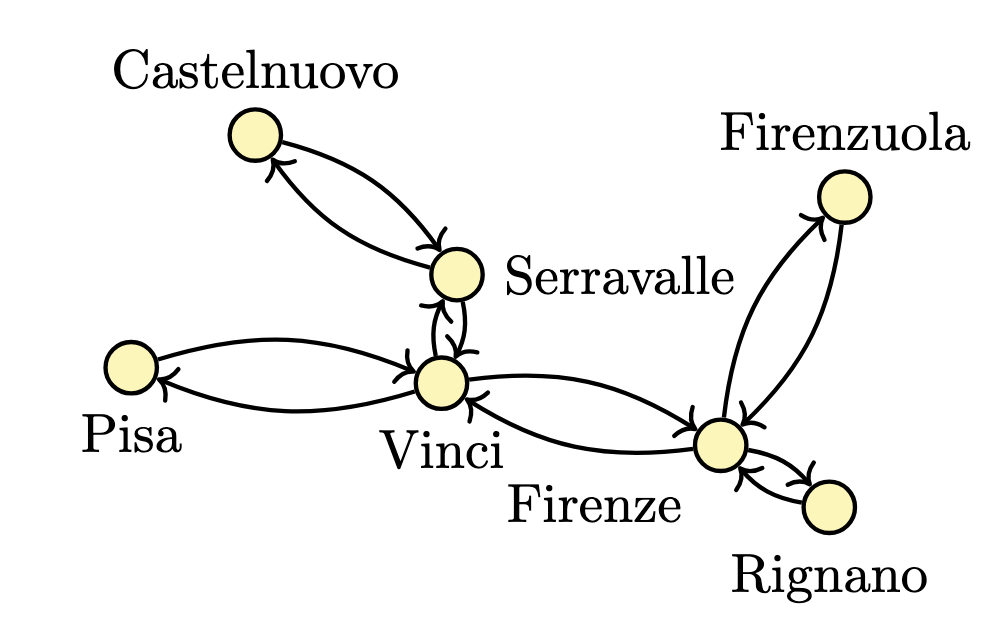
\includegraphics[width = 0.45\textwidth]{Images/delta tsp.png }
	      \end{center}
	\item Parto da un nodo a caso. Seguo archi dell'albero fino a quanto tornerei su nodo visitato.
	\item Ogni volta che finisco su un nodo visitato lo salto e continuo a seguire gli archi dell'albero
	\item Per i due teoremini visti prima,
	      \[
		      c\left(\pi \right) < 2 \cdot c\left(mst\right) < 2 \cdot c\left(\pi^{*}\right)
	      \]
	      dove
	      \begin{align*}
		      \underbracket[0.1ex]{c\left(\pi \right) < 2 \cdot c\left(mst\right)}_{\text{per disuguaglianza triangolare}} &  & \underbracket[0.1ex]{2 \cdot c\left(mst\right) < 2 \cdot c\left(\pi^{*}\right)}_{\text{per teorema mst}}
	      \end{align*}

\end{itemize}
Nota che è dimostrabile che non esiste un'approssimazione migliore di $ 2 $ per TSP generico. Per $ \Delta$-tsp è possibile un'approssimazione di $ \frac{3}{2} $
\subsection{TSP euristico}
\subsubsection{Shortest edge first}
\begin{itemize}
	\item Ordino archi in modo decrescente
	\item Per ogni arco, lo prendo se e solo se
	      \begin{itemize}
		      \item Non forma un ciclo
		      \item I suoi estremi sono nodi con selected out degree $ < 2 $, ossia che siano connessi ad al più un edge fra quelli selezionati
	      \end{itemize}
	\item Alla fine connetto i 2 nodi con selected out degree 1
\end{itemize}
Complessità: $ O\left(n^2 \log n\right) $
\subsubsection{Nearest neighbor}
\begin{itemize}
	\item Parto da un nodo a caso
	\item Seleziono la prossima città non visitata più vicina
\end{itemize}
Complessità: $ O\left(n^2\right) $
\subsection{TSP branch and bound}
Possiamo applicare una strategia branch and bound con un pruning aggressivo per risolvere il TSP-problem.
L'idea del branch and bound è quella di
\begin{itemize}
	\item Tengo traccia globalmente della soluzione migliore \verb|minCost| scoperta fin'ora
	\item Ad ogni step di decisione, calcolo il limite inferiore del prezzo necessario per concludere la soluzione. Lo chiamo \verb|lb| (\textit{lower bound}).
	\item Continuo a generare le combinazioni del sotoalbero se e solo se \verb|lb < minCost|
\end{itemize}
Quindi il trucco sta nel calcolare il limite inferiore del costo di un albero (\verb|lb|). In tsp possiamo
\begin{itemize}
	\item Nella soluzione parziale $ S $ abbiamo un path.
	\item Dobbiamo passare per tutti i rimanenti nodi.
	\item Nel migliore dei casi, passerò per ogni nodo, entrando per l'arco di peso minore e uscendo per l'arco di peso minore. Chiamo questa quantità \verb|transfer[h]|
	\item A questo costo c'è da aggiungere il costo per uscire dall'ultimo nodo di $ S $ e entrare nel suo primo. Il costo totale del \textit{lower bound} sarà dunque:
	      \[
		      \mathrm{lb}(d, S, i)=\operatorname{cost}[i]+\left\lceil\frac{\text { out }+\sum_{h \notin S} \operatorname{transfer}[h]+\text { last }}{2}\right\rceil
	      \]
\end{itemize}
\section{Dimostrazioni da sapere}
\begin{itemize}
	\item Master Theorem
	\item Analisi ammortizzata vettori dinamici
	\item Limite altezza alberi red black
	\item Complessità costruzione Heap
	\item Limite altezza utilizzando euristica sul rango
	\item Correttezza LCS
	\item Compressione di huffman
	\item Teorema di Bellman
	      i
	\item Selezione probabilistica
	      i
\end{itemize}







\end{document}
